\documentclass[conference]{IEEEtran}
\IEEEoverridecommandlockouts
% The preceding line is only needed to identify funding in the first footnote. If that is unneeded, please comment it out.



\usepackage{cite}
\usepackage{amsmath,amssymb,amsfonts}
\usepackage{algorithmic}
\usepackage{graphicx}
\usepackage{textcomp}
\usepackage{xcolor}
\usepackage{dblfloatfix}
\usepackage{multirow}
\usepackage{placeins}
\renewcommand{\IEEEkeywordsname}{Palabras clave}

\makeatletter
\makeatother
\def\BibTeX{{\rm B\kern-.05em{\sc i\kern-.025em b}\kern-.08em
    T\kern-.1667em\lower.7ex\hbox{E}\kern-.125emX}}
\begin{document}

\title{RF-DETR evaluation for Multispecies Detection in High Occluded Scenarios at African Savanna \\
}

\author{
\IEEEauthorblockN{1\textsuperscript{st} Amir Sadour}
\IEEEauthorblockA{\textit{MaIA} \\
\textit{Universidad de los Andes}\\
Bogotá, Colombia \\
a.sadour@uniandes.edu.co}
\and
\IEEEauthorblockN{2\textsuperscript{nd} Camilo Rodriguez}
\IEEEauthorblockA{\textit{MaIA} \\
\textit{Universidad de los Andes}\\
Bogotá, Colombia \\
ca.rodriguezs123@uniandes.edu.co}
\linebreak % <<---- fuerza el salto de línea
\and
\IEEEauthorblockN{3\textsuperscript{rd} Claudia Agudelo}
\IEEEauthorblockA{\textit{MaIA} \\
\textit{Universidad de los Andes}\\
Cali, Colombia \\
cj.agudelo@uniandes.edu.co}
\and
\IEEEauthorblockN{4\textsuperscript{th} Luis Manrique}
\IEEEauthorblockA{\textit{MaIA} \\
\textit{Universidad de los Andes}\\
Bogotá, Colombia \\
l.manriquec@uniandes.edu.co}
}


\maketitle

\begin{abstract}

%% This article addresses the challenge of automatic monitoring of wildlife in aerial imagery, specially on high density scenarios.
%% Este artículo aborda el desafío crítico del monitoreo automatizado de fauna silvestre en imágenes aéreas, específicamente en escenarios de alta densidad (manadas).
This article addresses the challenge of automated wildlife monitoring in aerial imagery, particularly in on high-density scenarios (herds).

% El problema central radica en que los detectores tradicionales basados en CNN fallan ante la oclusión y superposición de animales; el algoritmo de Supresión de No Máximos (NMS) tiende a eliminar detecciones válidas, provocando un subconteo sistemático, mientras que modelos como HerdNet, aunque evitan el NMS, luchan con la clasificación de especies minoritarias.
% The main challenge is because traditional detectors based on CNN architectures fails where animals are occluded or overwrite; the Non Maximal Suppression (NMS) tends to omit valid detections, causing a systematic sub-counting, while models like HerdNet which prevents the usage of NMS, face a challenge with under-represented species.  

The core problem relies on the fact that traditional CNN-based detectors fail in the presence of animal occlusion and overlap; specifically, Non-Maximum Suppression (NMS) tends to discard valid detections, resulting in systematic undercounting. Meanwhile, models such as HerdNet which bypass NMS, struggle with underrepresented species.

% Como solución, se propone la implementación de RF-DETR. Esta arquitectura utiliza mecanismos de atención para modelar dependencias globales y realiza una predicción de conjuntos end-to-end, lo que permite eliminar por completo la necesidad de NMS y gestionar mejor las oclusiones severas.
% As a solution, we propose a solution based on the RF-DETR architecture, which uses attention mechanisms to model global dependencies and predicts the object detections and classification end-to-end, removing hand crafted intermediate methods like NMS. Our bet is that it improves the scenes where severe occlusions are present.

To address this issue, this paper proposes a solution leveraging the RF-DETR architecture. By utilizing its attention mechanisms to model global dependencies and its end-to-end set prediction, our approach eliminates the need for NMS and provides more robust spatial data in severe occlusion scenarios.

% La metodología consistió en comparar tres variantes de RF-DETR (Nano, Small, Large) frente al modelo base HerdNet, utilizando un dataset de mamíferos africanos.
% The methodology consists in to compare three variants of RF-DETR based on the model size (Nano, Small, Large), over the last state of the art model HerdNet, which was built using an African mammal dataset. 
The methodology involved evaluating three RF-DETR variants -- Nano, Small and Large -- against the state of the art HerdNet baseline, utilizing a dataset of African mammals.

% Se aplicó una estrategia de entrenamiento en dos fases, donde la segunda etapa incorporó  Minería de Negativos Difíciles (HNM) para refinar la precisión y reducir falsos positivos en fondos complejos
% A two phases strategy were applied, on the first one we have trained with patches where strictly an animal is contained. The second phase incorporates Hard Negative Mining (HNM) to reduce false positives in complex backgrounds.   
A two-phase training strategy was implemented. The first phase utilized image patches containing only positive samples (animals). The second stage incorporated Hard Negative Mining (HNM) to refine precision and mitigate false positives in complex background.

%Los principales resultados determinaron que RF-DETR Small es la variante óptima.
% Results has shown that RF-DETR Small is the optimal variant.
% Este modelo alcanzó un F1-Score del 90.24\%, superando significativamente al baseline (83.26\%) y reduciendo el error medio de conteo (MAE) en un 39.47\%. Además, demostró ser un 56\% más rápido en inferencia que HerdNet y mejoró sustancialmente la detección de especies minoritarias (como el cobo de agua), validando la superioridad de los Transformers para equilibrar precisión y eficiencia en tareas de conservación.
The main results indicate that RF-DETR Small is the optimal variant. This model achieved an F1-Score of 90.24\%, significantly outperforming the baseline (83.26\%) and reducing the Mean Absolute Error (MAE) for counting by 39.47\%. Additionally, it demonstrated 56\% faster inference compared to HerdNet and substantially improved detection of minority species (such as waterbuck), validating the superiority of Transformers in balancing precision and efficiency for conservation tasks.\newline
\end{abstract}

\begin{IEEEkeywords}
%RF-DETR, HerdNet, DINOv2,HNM, detección de animales, imágenes aéreas, manadas densas
RF-DETR, HerdNet, DINOv2, HNM, animal detection, aerial imagery, dense herds

\end{IEEEkeywords}





%\section{Introducción}
%El monitoreo automatizado de la fauna silvestre mediante imágenes aéreas es crucial para la conservación ecológica, pero enfrenta un desafío crítico en la sabana africana: la detección precisa en escenarios de alta densidad. Especies gregarias como elefantes y búfalos forman manadas compactas con severa oclusión y superposición entre individuos, condiciones donde los sistemas de visión por computador convencionales fallan sistemáticamente.
%
%El problema fundamental radica en las arquitecturas tradicionales basadas en CNN y anclas, que dependen del algoritmo de Supresión de No Máximos (NMS). En manadas densas, el NMS elimina erróneamente detecciones válidas de animales contiguos, provocando un subconteo crónico. Aunque alternativas como HerdNet \cite{herdnet} evitan el NMS mediante la estimación de densidad por puntos, su dependencia de backbones CNN limita la captura del contexto global necesario para una clasificación robusta, afectando especialmente a las especies minoritarias.
%
%Este trabajo se justifica por la necesidad de una solución que supere simultáneamente las limitaciones de oclusión y discriminación semántica. El objetivo principal es implementar y evaluar la arquitectura \textbf{RF-DETR} (\textit{Real-Time Detection Transformer}) \cite{rf-detr} en este contexto desafiante. Nuestra hipótesis es que el mecanismo de atención de los Transformers, capaz de modelar dependencias globales, junto con la predicción de conjuntos \textit{end-to-end} que elimina por completo la necesidad del NMS, ofrece una solución estructural al problema del subconteo en manadas.
%
%Las principales contribuciones de este estudio son:  (1) Una comparación de tres variantes de RF-DETR (Nano, Small, Large) frente al baseline HerdNet. (2) Un análisis del compromiso entre precisión en alta densidad y costo computacional de las arquitecturas, identificando configuraciones óptimas para el despliegue práctico. (3) La validación de una estrategia de entrenamiento de dos fases con Minería de Negativos Difíciles (HNM) para refinar la precisión en fondos complejos.

\section{Introduction}
Automated wildlife monitoring using aerial imagery is crucial for ecological conservation, but faces a critical challenge in the African savanna: precise detection in high-density scenarios. Gregarious species such as elephants and buffalo form compact herds with severe occlusion and overlap between individuals, conditions where conventional computer vision systems systematically fail.

The fundamental problem lies in traditional CNN-based and anchor-based architectures, which rely on the Non-Maximum Suppression (NMS) algorithm. In dense herds, NMS erroneously eliminates valid detections of contiguous animals, causing chronic undercounting. Although alternatives such as HerdNet \cite{herdnet} avoid NMS through point-based density estimation, their dependence on CNN backbones limits the capture of global context necessary for robust classification, particularly affecting minority species.

This work is justified by the need for a solution that simultaneously overcomes the limitations of occlusion and semantic discrimination. The main objective is to implement and evaluate the \textbf{RF-DETR} (\textit{Real-Time Detection Transformer}) \cite{rf-detr} architecture in this challenging context. Our hypothesis is that the Transformer's attention mechanism, capable of modeling global dependencies, together with \textit{end-to-end} set prediction that completely eliminates the need for NMS, offers a structural solution to the undercounting problem in herds.

The main contributions of this study are: (1) A comparison of three RF-DETR variants (Nano, Small, Large) against the HerdNet baseline. (2) An analysis of the trade-off between precision in high density and computational cost of the architectures, identifying optimal configurations for practical deployment. (3) The validation of a two-phase training strategy with Hard Negative Mining (HNM) to refine precision in complex backgrounds.


% \section{Estado del arte}
\section{State of the Art}

% La monitorización de la fauna silvestre mediante imágenes aéreas ha evolucionado significativamente, pasando de métodos de conteo manual propensos a sesgos humanos a sistemas automatizados basados en visión por computador. La revisión de la literatura revela una transición tecnológica desde las Redes Neuronales Convolucionales (CNN) tradicionales hacia arquitecturas especializadas en densidad y, más recientemente, hacia modelos basados en Transformers y mecanismos de atención. A continuación, se describen los enfoques más relevantes y la evolución técnica que fundamenta este proyecto.
Wildlife monitoring through aerial imagery has evolved significantly, transitioning from manual counting methods prone to human biases to automated systems based on computer vision. The literature review reveals a technological transition from traditional Convolutional Neural Networks (CNNs) toward density-specialized architectures and, more recently, toward Transformer-based models and attention mechanisms. Below, we describe the most relevant approaches and the technical evolution that underlies this project.

% \subsection{Detección basada en CNNs y limitaciones en manadas densas}
\subsection{CNN-based Detection and Limitations in Dense Herds}

% Históricamente, la detección de animales en imágenes aéreas se ha abordado mediante detectores de objetos de propósito general basados en anclas (\textit{anchor-based}), como Faster R-CNN, Libra R-CNN y RetinaNet. Estudios previos sobre el mismo conjunto de datos utilizado en esta investigación demostraron que modelos como Libra R-CNN podían alcanzar una precisión media (mAP) del 80\% en condiciones ideales \cite{delplanque-data}.
Historically, animal detection in aerial images has been approached using general-purpose anchor-based object detectors, such as Faster R-CNN, Libra R-CNN, and RetinaNet. Previous studies on the same dataset used in this research demonstrated that models like Libra R-CNN could achieve a mean Average Precision (mAP) of 80\% under ideal conditions \cite{delplanque-data}.

% Sin embargo, como sintetizan diversas revisiones del campo \cite{xu-review}, estas arquitecturas presentan dos limitaciones fundamentales en el contexto de manadas densas:
However, as synthesized by various field reviews \cite{xu-review}, these architectures present two fundamental limitations in the context of dense herds:

% 1. Dependencia del NMS: el algoritmo de Supresión de No Máximos tiende a eliminar detecciones válidas cuando varios animales aparecen muy próximos, lo que provoca subconteo sistemático.
1. NMS Dependency: the Non-Maximum Suppression (NMS) algorithm tends to eliminate valid detections when several animals appear in close proximity, causing systematic undercounting.

% 2. Objetos pequeños y ocluidos: en imágenes aéreas, los animales suelen ocupar pocos píxeles, y las CNN tradicionales tienen dificultades para distinguir individuos contiguos en fondos heterogéneos.
2. Small and occluded objects: in aerial images, animals typically occupy few pixels, and traditional CNNs have difficulty distinguishing contiguous individuals against heterogeneous backgrounds.

% En estudios aplicados a fauna africana, Delplanque et al. observaron caídas críticas de precisión en grupos densos debido exactamente a estos factores \cite{delplanque-data}. Estas limitaciones motivaron el desarrollo de modelos específicamente diseñados para entornos con oclusión extrema.
In studies applied to African wildlife, Delplanque et al. observed critical drops in precision in dense groups due to exactly these factors \cite{delplanque-data}. These limitations motivated the development of models specifically designed for environments with extreme occlusion.

% \subsection{HerdNet y el enfoque basado en puntos}
\subsection{HerdNet and the Point-based Approach}

% Para resolver el dilema entre la localización precisa y el conteo en masas, Delplanque et al. propusieron \textbf{HerdNet}, el cual se establece como el modelo de referencia (\textit{baseline}) para este proyecto \cite{herdnet}. HerdNet abandona el enfoque de cajas delimitadoras en favor de una estimación basada en puntos, inspirada en técnicas de conteo de multitudes (\textit{crowd counting}).
To resolve the dilemma between precise localization and mass counting, Delplanque et al. proposed \textbf{HerdNet}, which is established as the baseline model for this project \cite{herdnet}. HerdNet abandons the bounding box approach in favor of point-based estimation, inspired by crowd counting techniques.

% Esta arquitectura utiliza un mapa de Transformada de Distancia Inversa Focal (FIDT).Este mapa genera picos localizados en el centro de cada animal, permitiendo detectar individuos incluso cuando no hay contornos claros, evitar por completo el uso de NMS, y mantener robustez en presencia de oclusiones y variaciones de escala.
This architecture uses a Focal Inverse Distance Transform (FIDT) map. This map generates localized peaks at the center of each animal, enabling the detection of individuals even when there are no clear contours, completely avoiding the use of NMS, and maintaining robustness in the presence of occlusions and scale variations.

% Aunque HerdNet superó a las arquitecturas basadas en anclas (como Faster R-CNN) y basadas en densidad pura (como DLA-34) con un F1-Score del 73.6\% y un RMSE de 9.8, sobre el conjunto de datos de múltiples especies utilizado en este proyecto, presenta desafíos en la clasificación de especies minoritarias y una dependencia de arquitecturas de CNN convencionales que pueden no capturar eficazmente el contexto global de la imagen.
Although HerdNet outperformed anchor-based architectures (such as Faster R-CNN) and pure density-based architectures (such as DLA-34) with an F1-Score of 73.6\% and an RMSE of 9.8 on the multi-species dataset used in this project, it presents challenges in classifying minority species and a dependence on conventional CNN architectures that may not effectively capture the global context of the image.

% \subsection{La revolución de los Transformers: WildlifeMapper, OpenWildlife y RF-DETR}
\subsection{The Transformer Revolution: WildlifeMapper, OpenWildlife, and RF-DETR}

% La incorporación de arquitecturas tipo \textit{Transformer} ha marcado un punto de inflexión en la detección de objetos en imágenes aéreas. A diferencia de las CNN convencionales, estos modelos introducen mecanismos de atención capaces de capturar relaciones espaciales de largo alcance, lo que resulta crítico para manejar variaciones extremas de escala y fondos heterogéneos.
The incorporation of \textit{Transformer}-type architectures has marked a turning point in object detection in aerial images. Unlike conventional CNNs, these models introduce attention mechanisms capable of capturing long-range spatial relationships, which is critical for handling extreme scale variations and heterogeneous backgrounds.

% \subsubsection*{WildlifeMapper y OpenWildlife}
\subsubsection*{WildlifeMapper and OpenWildlife}
% Kumar et al. presentaron \textbf{WildlifeMapper} \cite{wildlife-mapper}, una arquitectura que integra módulos de refinamiento local para capturar estructuras de alta frecuencia. Este enfoque ha demostrado ser superior en el manejo de imágenes aéreas de muy alta resolución (hasta $8400 \times 5500$ px), permitiendo una localización precisa en paisajes vastos.
Kumar et al. presented \textbf{WildlifeMapper} \cite{wildlife-mapper}, an architecture that integrates local refinement modules to capture high-frequency structures. This approach has proven superior in handling very high-resolution aerial images (up to $8400 \times 5500$ px), enabling precise localization in vast landscapes.

% Por otro lado, Patel et al. propusieron \textbf{OpenWildlife} \cite{open-wildlife}, un detector de vocabulario abierto basado en la arquitectura \textit{Grounding-DINO}. Este modelo combina un \textit{backbone} visual (Swin Transformer) con un codificador de lenguaje (BERT), permitiendo la detección de fauna guiada por descripciones textuales naturales. Si bien ofrece una gran capacidad de generalización hacia especies no vistas durante el entrenamiento, su arquitectura pesada conlleva un costo computacional que limita su escalabilidad en análisis masivos.
On the other hand, Patel et al. proposed \textbf{OpenWildlife} \cite{open-wildlife}, an open-vocabulary detector based on the \textit{Grounding-DINO} architecture. This model combines a visual \textit{backbone} (Swin Transformer) with a language encoder (BERT), enabling wildlife detection guided by natural textual descriptions. While it offers great generalization capacity toward species not seen during training, its heavy architecture entails a computational cost that limits its scalability in massive analyses.

% \subsubsection*{RF-DETR: Eficiencia en Tiempo Real}
\subsubsection*{RF-DETR: Real-Time Efficiency}
% Más recientemente, Robinson et al. introdujeron \textbf{RF-DETR} \cite{rf-detr}, un \textit{Detection Transformer} diseñado específicamente para optimizar el equilibrio entre precisión y latencia. Esta arquitectura se distingue por dos innovaciones clave:
More recently, Robinson et al. introduced \textbf{RF-DETR} \cite{rf-detr}, a \textit{Detection Transformer} designed specifically to optimize the balance between accuracy and latency. This architecture is distinguished by two key innovations:

\begin{itemize}
    % \item \textbf{Búsqueda de Arquitectura Neuronal (NAS) de peso compartido:} Permite ajustar dinámicamente la profundidad del decodificador, el número de \textit{queries} y las ventanas de atención sin necesidad de reentrenar el modelo desde cero.
    \item \textbf{Weight-shared Neural Architecture Search (NAS):} Allows dynamically adjusting the decoder depth, number of \textit{queries}, and attention windows without needing to retrain the model from scratch.
    % \item \textbf{Backbone DINOv2 \cite{dinov2}:} Incorpora representaciones visuales robustas obtenidas mediante un preentrenamiento autosupervisado a escala de internet.
    \item \textbf{DINOv2 Backbone \cite{dinov2}:} Incorporates robust visual representations obtained through internet-scale self-supervised pretraining.
\end{itemize}

% En benchmarks estándar como COCO y el complejo RF100-VL, RF-DETR ha superado a detectores modernos como YOLOv8 y D-FINE, logrando métricas superiores a 60 AP con latencias por debajo de los 40 ms \cite{rf-detr}. Crucialmente para este proyecto, RF-DETR opera como un detector \textit{end-to-end}, eliminando la necesidad de algoritmos de post-procesamiento manuales como la Supresión de No Máximos (NMS). Esta característica lo hace teóricamente superior en escenarios de alta densidad, donde el NMS tradicional tiende a suprimir individuos contiguos.
On standard benchmarks such as COCO and the complex RF100-VL, RF-DETR has surpassed modern detectors like YOLOv8 and D-FINE, achieving metrics above 60 AP with latencies below 40 ms \cite{rf-detr}. Crucially for this project, RF-DETR operates as an \textit{end-to-end} detector, eliminating the need for manual post-processing algorithms such as Non-Maximum Suppression (NMS). This characteristic makes it theoretically superior in high-density scenarios, where traditional NMS tends to suppress contiguous individuals.

% \subsection{Análisis, brechas identificadas y propuesta}
\subsection{Analysis, Identified Gaps, and Proposal}

% La revisión exhaustiva de la literatura permite identificar tres brechas tecnológicas principales que limitan el monitoreo automatizado de fauna en la actualidad:
The exhaustive review of the literature allows us to identify three main technological gaps that currently limit automated wildlife monitoring:

\begin{enumerate}
    % \item \textbf{Precisión limitada en densidad extrema:} Los modelos tradicionales basados en anclas (como la familia YOLO o Faster R-CNN) fallan sistemáticamente en la detección de manadas densas. Esto se debe intrínsecamente al uso de NMS, que al intentar eliminar duplicados, elimina erróneamente detecciones válidas de animales que se superponen o están muy próximos entre sí \cite{xu-review}.
    \item \textbf{Limited precision in extreme density:} Traditional anchor-based models (such as the YOLO family or Faster R-CNN) systematically fail in detecting dense herds. This is intrinsically due to the use of NMS, which, when attempting to eliminate duplicates, erroneously eliminates valid detections of animals that overlap or are in very close proximity to each other \cite{xu-review}.

    % \item \textbf{Dilema entre localización y contexto semántico:} Enfoques como HerdNet \cite{herdnet} resolvieron eficazmente el problema de la oclusión mediante la estimación de densidad basada en puntos. Sin embargo, al depender de CNNs tradicionales, su capacidad para capturar el contexto global de la imagen es limitada, lo que afecta su capacidad de generalización y clasificación fina en entornos complejos.
    \item \textbf{Dilemma between localization and semantic context:} Approaches like HerdNet \cite{herdnet} effectively solved the occlusion problem through point-based density estimation. However, by relying on traditional CNNs, their ability to capture the global context of the image is limited, affecting their generalization capacity and fine-grained classification in complex environments.

    % \item \textbf{Costo computacional de los modelos fundacionales:} Aunque métodos recientes como WildlifeMapper y OpenWildlife ofrecen un desempeño excelente y capacidades de vocabulario abierto, sus requerimientos computacionales son prohibitivos para el despliegue en escenarios de conservación con recursos limitados o para el procesamiento de grandes volúmenes de datos de drones \cite{open-wildlife}.
    \item \textbf{Computational cost of foundation models:} Although recent methods like WildlifeMapper and OpenWildlife offer excellent performance and open-vocabulary capabilities, their computational requirements are prohibitive for deployment in resource-limited conservation scenarios or for processing large volumes of drone data \cite{open-wildlife}.
\end{enumerate}

% \textbf{Síntesis y propuesta de valor:}
\textbf{Synthesis and value proposal:}
% El análisis de estas limitaciones sugiere que existe una oportunidad no explorada en la intersección de estas tecnologías. Se plantea que la implementación de \textbf{RF-DETR} en el contexto de manadas densas podría cerrar estas brechas simultáneamente.
The analysis of these limitations suggests that there is an unexplored opportunity at the intersection of these technologies. It is proposed that the implementation of \textbf{RF-DETR} in the context of dense herds could close these gaps simultaneously.

% La hipótesis central es que la capacidad de los Transformers para modelar relaciones globales y prescindir del NMS permitirá mejorar la recuperación (\textit{recall}) de individuos en manadas densas, superando el conteo de HerdNet. Simultáneamente, se espera que el uso de un \textit{backbone} robusto como DINOv2 mejore la discriminación entre especies (reduciendo la confusión reportada en HerdNet), todo ello manteniendo una eficiencia computacional viable para su aplicación práctica.
The central hypothesis is that the ability of Transformers to model global relationships and dispense with NMS will improve the recovery (\textit{recall}) of individuals in dense herds, surpassing HerdNet's counting. Simultaneously, it is expected that the use of a robust \textit{backbone} like DINOv2 will improve discrimination between species (reducing the confusion reported in HerdNet), all while maintaining computationally viable efficiency for practical application.

\begin{figure*}[t!]
    \centering
    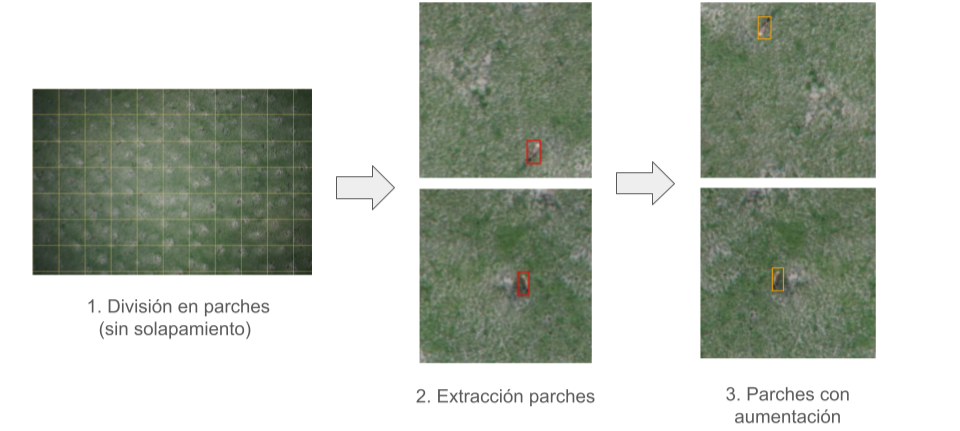
\includegraphics[width=0.8\textwidth]{static/img/aumento.png}
    % \caption{Visualización del preprocesamiento: extracción de recortes (tiling) y ejemplos de aumentación de datos aplicados para el entrenamiento de HerdNet y RF-DETR.}
    \caption{Preprocessing visualization: tile extraction (tiling) and examples of data augmentation applied for HerdNet and RF-DETR training.}
    \label{fig:preprocessing}
\end{figure*}


% \section{Metodología}
\section{Methodology}

% La metodología adoptada sigue el ciclo de vida estándar de un proyecto de aprendizaje automático, estructurándose en cuatro fases principales: preparación de datos, modelado y experimentación, estrategia de entrenamiento y despliegue. El enfoque se centró en superar las limitaciones de los detectores tradicionales en escenarios de alta densidad mediante la implementación de arquitecturas basadas en Transformers con optimización de arquitectura neuronal (NAS).
The adopted methodology follows the standard life cycle of a machine learning project, structured in four main phases: data preparation, modeling and experimentation, training strategy, and deployment. The approach focused on overcoming the limitations of traditional detectors in high-density scenarios through the implementation of Transformer-based architectures with Neural Architecture Search (NAS).

% \subsection{Gestión y Procesamiento de Datos}
\subsection{Data Management and Processing}

% \subsubsection{Descripción del Dataset}
\subsubsection{Dataset Description}

% Se utilizó el conjunto de datos consolidado por Delplanque et al. \cite{delplanque-data}, el cual agrega 10.239 anotaciones de mamíferos africanos provenientes de dos fuentes principales: el Parque Nacional Virunga (RDC) y el \textit{Aerial Elephant Dataset} (AED). El dataset incluye seis clases de especies objetivo: Búfalo, Elefante, Kob, Topi, Facóquero y Cobo de agua.
We used the dataset consolidated by Delplanque et al. \cite{delplanque-data}, which aggregates 10,239 annotations of African mammals from two main sources: Virunga National Park (DRC) and the \textit{Aerial Elephant Dataset} (AED). The dataset includes six target species classes: Buffalo, Elephant, Kob, Topi, Warthog, and Waterbuck.

% Las imágenes se caracterizan por una vista cenital con una resolución espacial muy alta, presentando un \textit{Ground Sampling Distance} (GSD) que varía entre 2.4 cm y 13 cm por píxel. El conjunto de datos presenta un desafío significativo de desbalance de clases, donde especies mayoritarias como el elefante superan en proporción 12:1 a especies minoritarias como el cobo de agua. La distribución detallada de individuos por especie y su división en los conjuntos de entrenamiento, validación y prueba se presenta en la tabla \ref{tab:dataset_dist}.
The images are characterized by a top-down view with very high spatial resolution, featuring a \textit{Ground Sampling Distance} (GSD) that varies between 2.4 cm and 13 cm per pixel. The dataset presents a significant class imbalance challenge, where majority species such as elephant exceed minority species such as waterbuck in a 12:1 ratio. The detailed distribution of individuals per species and their division into training, validation, and test sets is presented in Table \ref{tab:dataset_dist}.

\begin{table}[ht]
\centering
% \caption{Distribución de individuos por especie en los conjuntos de entrenamiento, validación y prueba.}
\caption{Distribution of individuals per species in the training, validation, and test sets.}
\label{tab:dataset_dist}
% Usamos \columnwidth para asegurar que la tabla se ajuste al ancho de una sola columna
\resizebox{\columnwidth}{!}{%
\begin{tabular}{lcccc}
\hline
\textbf{Especie} & \textbf{Entrenamiento} & \textbf{Validación} & \textbf{Prueba} & \textbf{Total} \\ \hline
Búfalo & 1058 (70\%) & 102 (7\%) & 349 (23\%) & 1509 \\
Elefante & 2012 (68\%) & 264 (9\%) & 688 (23\%) & 2964 \\
Kob & 1732 (73\%) & 161 (7\%) & 477 (20\%) & 2370 \\
Topi & 1678 (62\%) & 369 (13\%) & 675 (25\%) & 2722 \\
Facóquero & 316 (73\%) & 43 (10\%) & 74 (17\%) & 433 \\
Cobo de agua & 166 (69\%) & 39 (16\%) & 36 (15\%) & 241 \\ \hline
\textbf{Total} & \textbf{6962 (68\%)} & \textbf{978 (10\%)} & \textbf{2299 (22\%)} & \textbf{10 239} \\ \hline
\end{tabular}%
}
\end{table}


% \subsubsection{Preprocesamiento y Aumento de Datos}
\subsubsection{Preprocessing and Data Augmentation}

% Dada la alta resolución de las imágenes aéreas originales, se implementó una estrategia de \textit{tiling} (teselado) adaptativa. Para alinearse con las arquitecturas de los modelos seleccionados, se generaron recortes (\textit{patches}) en tres resoluciones específicas: $384 \times 384$, $512 \times 512$ y $560 \times 560$ píxeles. Se mantuvo un solapamiento (\textit{overlap}) estratégico entre teselas para evitar el corte de animales en los bordes de la imagen.
Given the high resolution of the original aerial images, an adaptive \textit{tiling} strategy was implemented. To align with the architectures of the selected models, crops (\textit{patches}) were generated in three specific resolutions: $384 \times 384$, $512 \times 512$, and $560 \times 560$ pixels. A strategic \textit{overlap} between tiles was maintained to avoid cutting animals at image edges.

% Para mejorar la robustez del modelo, se aplicó un pipeline de aumento de datos (\textit{data augmentation}) que incluyó:
To improve model robustness, a \textit{data augmentation} pipeline was applied that included:
\begin{itemize}
%     \item \textbf{Transformaciones geométricas:} Rotaciones aleatorias, volteo horizontal/vertical y recortes aleatorios.
    \item \textbf{Geometric transformations:} Random rotations, horizontal/vertical flipping, and random crops.
%     \item \textbf{Transformaciones fotométricas:} Ajustes de brillo, contraste y saturación para simular la variabilidad lumínica.
    \item \textbf{Photometric transformations:} Brightness, contrast, and saturation adjustments to simulate lighting variability.
\end{itemize}

% \subsection{Arquitecturas de Modelado}
\subsection{Modeling Architectures}

% \subsubsection{Modelo de Referencia (Baseline): HerdNet}
\subsubsection{Reference Model (Baseline): HerdNet}

% Para establecer una línea base rigurosa, se replicó la arquitectura \textbf{HerdNet} utilizando los scripts y clases definidos en su repositorio oficial \cite{herdnet}. Este modelo es una adaptación de la arquitectura \textit{CenterNet} diseñada específicamente para el conteo de multitudes, que abandona las cajas delimitadoras (bounding boxes) en favor de una estimación basada en puntos.
To establish a rigorous baseline, the \textbf{HerdNet} architecture was replicated using the scripts and classes defined in its official repository \cite{herdnet}. This model is an adaptation of the \textit{CenterNet} architecture designed specifically for crowd counting, which abandons bounding boxes in favor of point-based estimation.

% Como se ilustra en la Figura \ref{fig:herdnet_arch}, la arquitectura consta de un codificador-decodificador basado en \textbf{DLA-34} (Deep Layer Aggregation), el cual bifurca el procesamiento en dos ramas especializadas:
As illustrated in Figure \ref{fig:herdnet_arch}, the architecture consists of an encoder-decoder based on \textbf{DLA-34} (Deep Layer Aggregation), which bifurcates the processing into two specialized branches:

\begin{enumerate}
%     \item \textbf{Rama de Localización (Localization Map):} Genera un mapa de densidad de alta resolución ($256 \times 256$ píxeles para una entrada de $512 \times 512$) utilizando la Transformada de Distancia Inversa Focal (FIDT). Este mapa predice picos de densidad en el centro de cada animal, permitiendo separar individuos en aglomeraciones densas donde las cajas delimitadoras se solaparían significativamente.
    \item \textbf{Localization Branch (Localization Map):} Generates a high-resolution density map ($256 \times 256$ pixels for a $512 \times 512$ input) using the Focal Inverse Distance Transform (FIDT). This map predicts density peaks at the center of each animal, allowing separation of individuals in dense agglomerations where bounding boxes would significantly overlap.
%     \item \textbf{Rama de Clasificación (Classification Maps):} Produce mapas de menor resolución ($16 \times 16$ píxeles) que contienen la información semántica de la especie. Durante la inferencia, el modelo utiliza una Estrategia de Detección de Máximos Locales (LMDS) para extraer las coordenadas precisas del mapa de localización y asignarles la clase correspondiente del mapa de clasificación.
    \item \textbf{Classification Branch (Classification Maps):} Produces lower-resolution maps ($16 \times 16$ pixels) that contain the semantic information of the species. During inference, the model uses a Local Maximum Detection Strategy (LMDS) to extract precise coordinates from the localization map and assign them the corresponding class from the classification map.
\end{enumerate}


\begin{figure}[ht!]
    \centering
    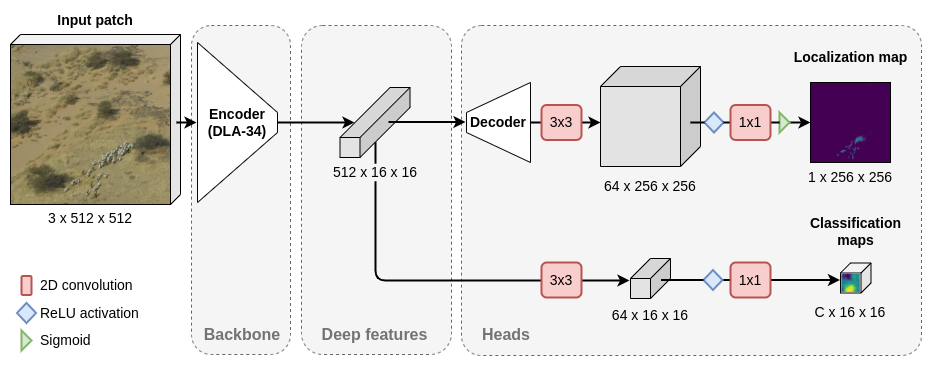
\includegraphics[width=\columnwidth]{static/img/herdnet_architecture.png} % Asegúrate de nombrar así tu archivo
%     \caption{Arquitectura de HerdNet. El modelo utiliza un backbone DLA-34 y se divide en dos cabezales: uno para generar un mapa de localización de alta resolución (arriba) y otro para mapas de clasificación de baja resolución (abajo) \cite{herdnet}.}
    \caption{HerdNet architecture. The model uses a DLA-34 backbone and is divided into two heads: one to generate a high-resolution localization map (top) and another for low-resolution classification maps (bottom) \cite{herdnet}.}
    \label{fig:herdnet_arch}
\end{figure}


% \subsubsection{Modelo Propuesto: RF-DETR}
\subsubsection{Proposed Model: RF-DETR}

% La solución propuesta se basa en \textbf{RF-DETR}, una arquitectura diseñada para optimizar el equilibrio entre precisión y latencia en aplicaciones de tiempo real. Como se ilustra en la Figura \ref{fig:rfdetr_arch}, su diseño integra componentes avanzados para mejorar la generalización y el manejo de oclusiones:
The proposed solution is based on \textbf{RF-DETR}, an architecture designed to optimize the balance between accuracy and latency in real-time applications. As illustrated in Figure \ref{fig:rfdetr_arch}, its design integrates advanced components to improve generalization and occlusion handling:

\begin{itemize}
%     \item \textbf{Backbone DINOv2:} Utiliza un \textit{Vision Transformer} (ViT-L/14) pre-entrenado con aprendizaje autosupervisado. Este backbone provee representaciones visuales robustas que facilitan la adaptación a dominios específicos con pocos datos anotados.
    \item \textbf{DINOv2 Backbone:} Uses a \textit{Vision Transformer} (ViT-L/14) pre-trained with self-supervised learning. This backbone provides robust visual representations that facilitate adaptation to specific domains with few annotated data.
%     \item \textbf{Extracción de Características Uniescala:} A diferencia de otros Transformers que procesan múltiples escalas, RF-DETR emplea una estrategia de extracción de características de una sola escala (ej. $640 \times 1280$ px) para reducir la sobrecarga computacional sin sacrificar significativamente la precisión.
    \item \textbf{Single-Scale Feature Extraction:} Unlike other Transformers that process multiple scales, RF-DETR employs a single-scale feature extraction strategy (e.g., $640 \times 1280$ px) to reduce computational overhead without significantly sacrificing accuracy.
%     \item \textbf{Cabezal Transformer y Atención Deformable:} Incorpora un mecanismo de atención cruzada deformable (\textit{Deformable Cross-Attention}) en el decodificador. Esto permite al modelo enfocarse selectivamente en características espacialmente relevantes, mejorando la detección en condiciones de oclusión severa, desorden visual (\textit{clutter}) y camuflaje, típicas de las manadas densas en la sabana.
    \item \textbf{Transformer Head and Deformable Attention:} Incorporates a \textit{Deformable Cross-Attention} mechanism in the decoder. This allows the model to selectively focus on spatially relevant features, improving detection in conditions of severe occlusion, visual \textit{clutter}, and camouflage, typical of dense herds in the savanna.
%     \item \textbf{Predicción de Conjuntos sin NMS:} El modelo realiza una predicción directa de conjuntos de cajas delimitadoras, eliminando la necesidad de anclajes (\textit{anchor boxes}) y de la Supresión de No Máximos (NMS). Esto es crítico para resolver el problema de subconteo en manadas densas, donde el NMS tradicional suprimiría detecciones válidas muy próximas.
    \item \textbf{Set Prediction without NMS:} The model performs direct set prediction of bounding boxes, eliminating the need for \textit{anchor boxes} and Non-Maximum Suppression (NMS). This is critical to solve the undercounting problem in dense herds, where traditional NMS would suppress valid detections in close proximity.
%     \item \textbf{Variantes:} Para evaluar el compromiso entre precisión y costo, se implementaron tres variantes: Nano (384 px), Small (512 px) y Large (560 px), permitiendo adaptar la complejidad del modelo a los recursos disponibles.
    \item \textbf{Variants:} To evaluate the tradeoff between accuracy and cost, three variants were implemented: Nano (384 px), Small (512 px), and Large (560 px), allowing the model complexity to be adapted to available resources.
\end{itemize}

\begin{figure*}[ht]
    \centering
    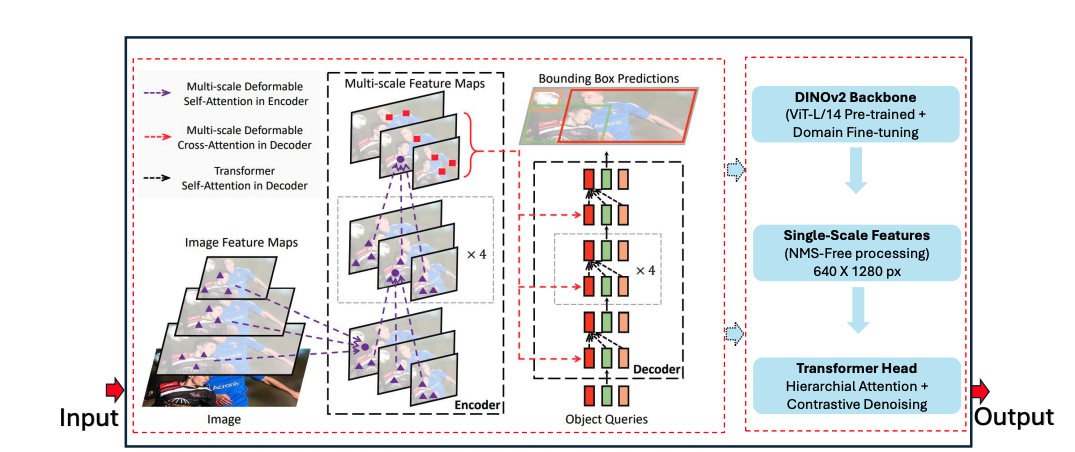
\includegraphics[width=0.93\textwidth]{static/img/rfdetr_architecture.png}
%     \caption{Arquitectura de RF-DETR para la detección de objetos. Muestra el flujo desde el backbone DINOv2, pasando por la extracción de características uniescala, hasta el cabezal Transformer con atención jerárquica y eliminación de ruido contrastivo. \cite{rf-detr}}
    \caption{RF-DETR architecture for object detection. Shows the flow from the DINOv2 backbone, through single-scale feature extraction, to the Transformer head with hierarchical attention and contrastive noise elimination. \cite{rf-detr}}
    \label{fig:rfdetr_arch}
\end{figure*}


% \subsection{Estrategia de Entrenamiento}
\subsection{Training Strategy}

\begin{figure}[ht]
    \centering
    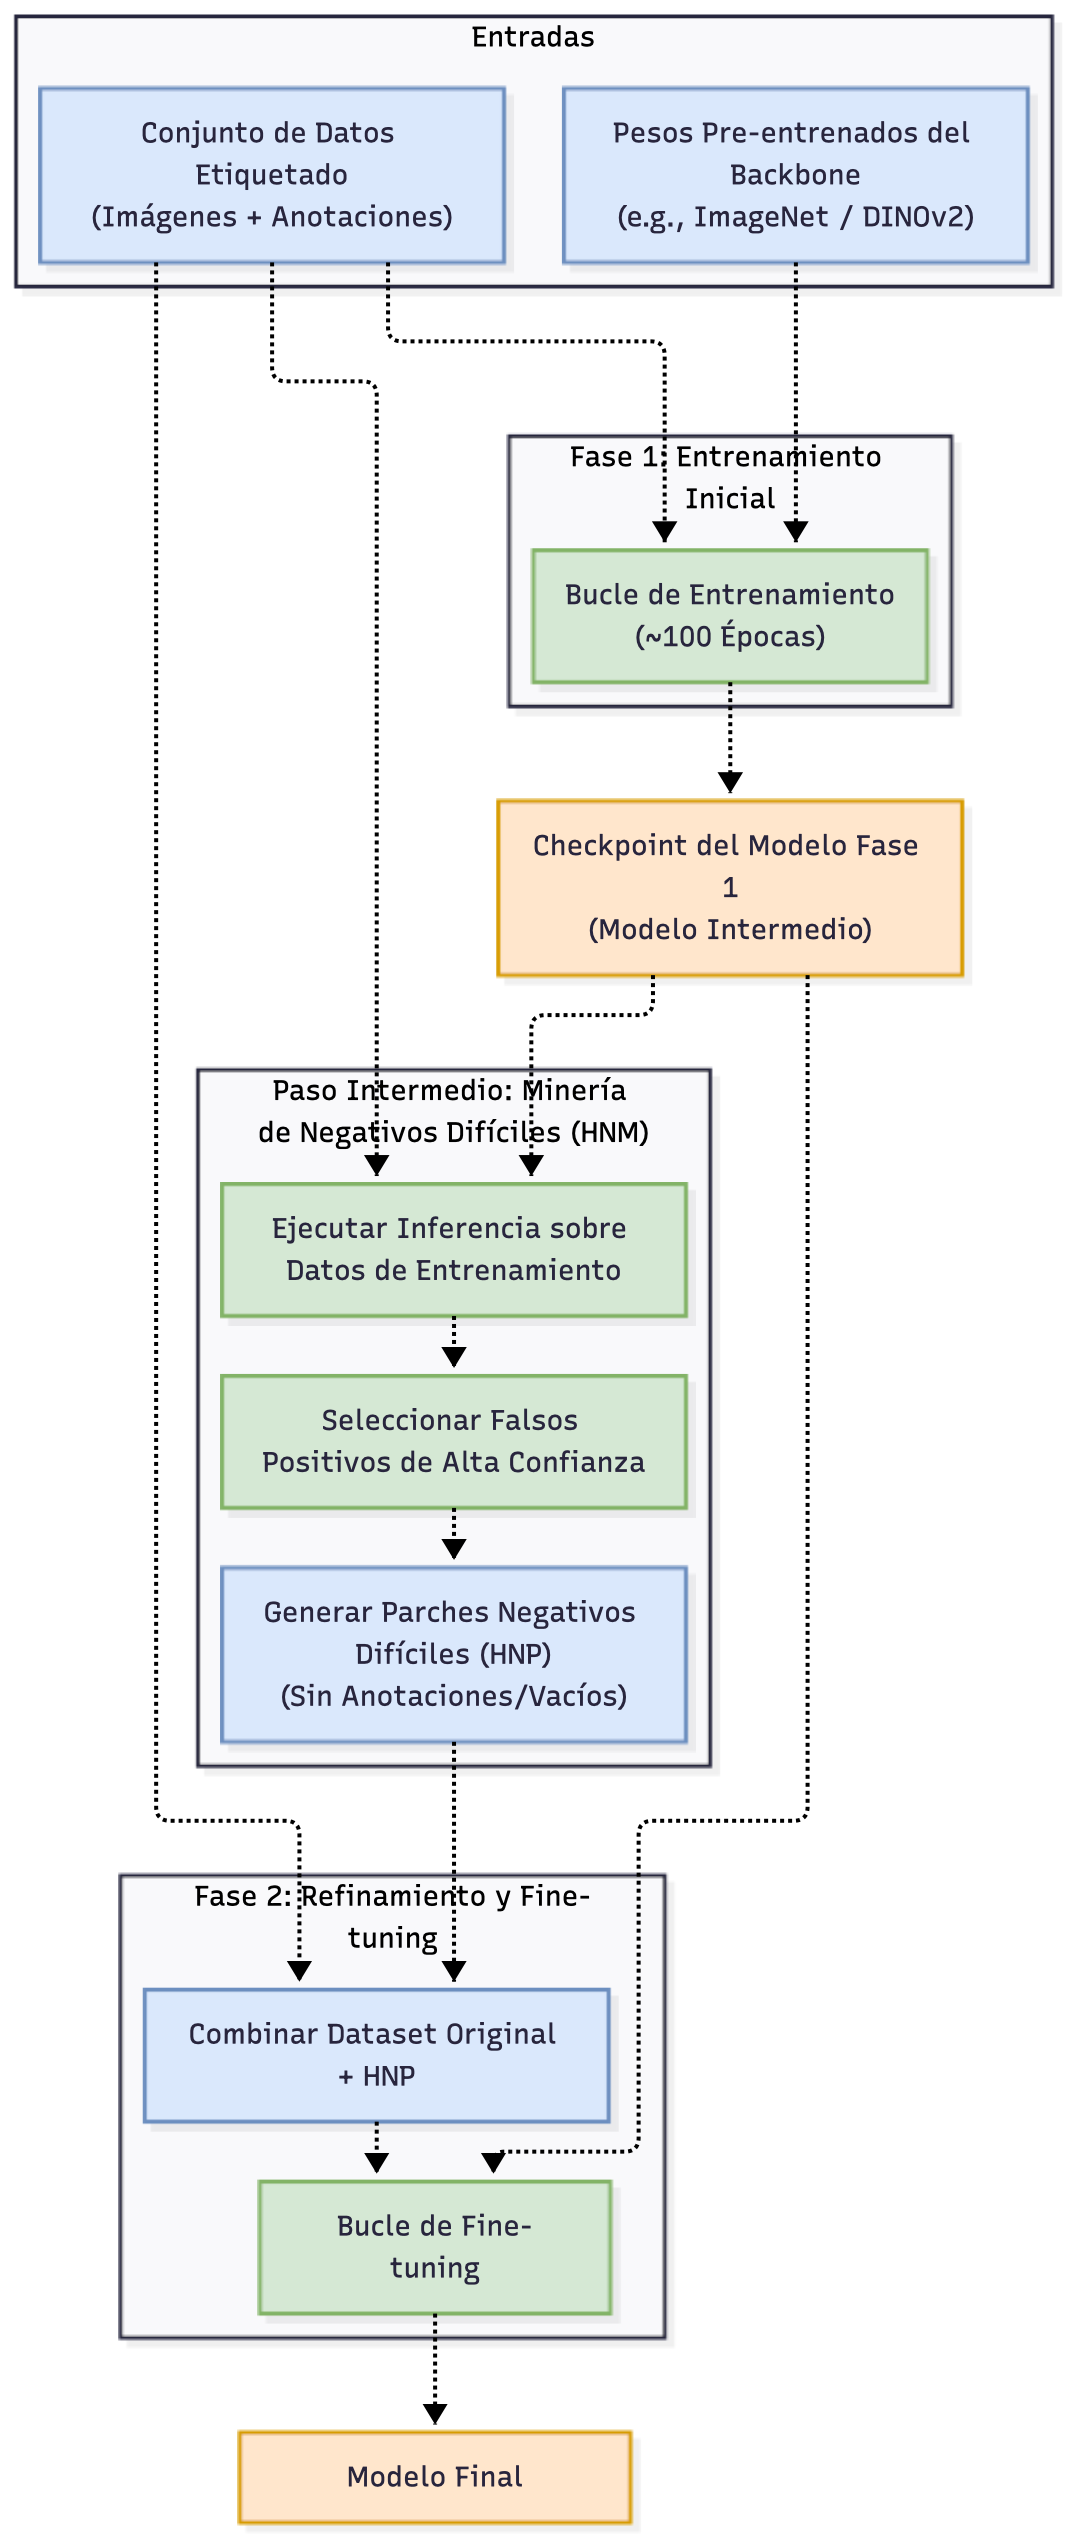
\includegraphics[width=0.35\textwidth, height=0.48\textheight]{static/img/entrenamiento.png}
%     \caption{Flujo de entrenamiento.}
    \caption{Training flow.}
    \label{fig:deployment_arch}
\end{figure}


% Se diseñó un protocolo dividido en dos etapas principales: la replicación del \textit{baseline} y el entrenamiento especializado del modelo propuesto, adaptando la técnica de minería de negativos difíciles (\textit{Hard Negative Mining}) para maximizar la precisión.
A protocol was designed divided into two main stages: the replication of the \textit{baseline} and the specialized training of the proposed model, adapting the \textit{Hard Negative Mining} technique to maximize accuracy.

% \subsubsection{Replicación de HerdNet}
\subsubsection{HerdNet Replication}

% El proceso se realizó en dos fases secuenciales:
The process was carried out in two sequential phases:
\begin{enumerate}
%     \item \textbf{Fase 1 (Entrenamiento Inicial):} Se entrenó el modelo durante 100 épocas con un \textit{learning rate} inicial de $1\times10^{-4}$ y un optimizador AdamW. La función de pérdida combinó \textit{Focal Loss} para la localización y \textit{Cross Entropy Loss} ponderada para la clasificación, asignando pesos específicos ($w=[0.1; 1.0; 2.0; \dots]$) para mitigar el desbalance de clases.
    \item \textbf{Phase 1 (Initial Training):} The model was trained for 100 epochs with an initial \textit{learning rate} of $1\times10^{-4}$ and an AdamW optimizer. The loss function combined \textit{Focal Loss} for localization and weighted \textit{Cross Entropy Loss} for classification, assigning specific weights ($w=[0.1; 1.0; 2.0; \dots]$) to mitigate class imbalance.
%     \item \textbf{Fase 2 (Refinamiento con HNP):} Se realizó un segundo entrenamiento de 50 épocas con una tasa de aprendizaje reducida a $1\times10^{-6}$. En esta etapa se introdujeron los parches negativos difíciles (\textit{Hard Negative Patches} - HNP), generados al ejecutar el modelo de la Fase 1 sobre las imágenes de entrenamiento y recolectar las predicciones de falsos positivos con alta confianza.
    \item \textbf{Phase 2 (Refinement with HNP):} A second training of 50 epochs was performed with a learning rate reduced to $1\times10^{-6}$. In this stage, \textit{Hard Negative Patches} (HNP) were introduced, generated by running the Phase 1 model on the training images and collecting high-confidence false positive predictions.
\end{enumerate}

% \subsubsection{Adaptación para RF-DETR}
\subsubsection{Adaptation for RF-DETR}

% Se replicó la estrategia de dos fases de HerdNet con las siguientes adaptaciones para la arquitectura Transformer:
The two-phase strategy of HerdNet was replicated with the following adaptations for the Transformer architecture:

% \paragraph{Hiperparámetros de Entrenamiento}
\paragraph{Training Hyperparameters}

% \textbf{Fase 1:} Se utilizó el \textit{backbone} DINOv2 pre-entrenado con normalización ImageNet y learning rate por defecto del framework (con decaimiento por capas). Se implementó un callback personalizado para monitorear métricas de HerdNet durante el entrenamiento.
\textbf{Phase 1:} The pre-trained DINOv2 \textit{backbone} was used with ImageNet normalization and the framework's default learning rate (with layer-wise decay). A custom callback was implemented to monitor HerdNet metrics during training.

% \textbf{Fase 2:} Fine-tuning con learning rate reducido ($1 \times 10^{-5}$ para las tres variantes), aumentación multi-escala activada, y regularización mediante weight decay y EMA. El dataset ampliado con HNP mantuvo las anotaciones originales solo en los parches positivos, forzando al modelo a predecir ausencia de objetos en regiones visualmente confusas.
\textbf{Phase 2:} Fine-tuning with reduced learning rate ($1 \times 10^{-5}$ for the three variants), multi-scale augmentation enabled, and regularization through weight decay and EMA. The dataset augmented with HNP maintained the original annotations only in positive patches, forcing the model to predict absence of objects in visually confusing regions.


% \paragraph{Inferencia y Evaluación}
\paragraph{Inference and Evaluation}

% Se empleó un \texttt{SimpleStitcher} para procesar imágenes completas en ventanas deslizantes y reconstruir detecciones en coordenadas originales. Las métricas se calcularon con el framework de HerdNet (radio de 20 píxeles) para mantener comparabilidad directa.
A \texttt{SimpleStitcher} was used to process complete images in sliding windows and reconstruct detections in original coordinates. Metrics were calculated with the HerdNet framework (20-pixel radius) to maintain direct comparability.

% \subsection{Herramientas y Despliegue}
\subsection{Tools and Deployment}

% El desarrollo de la solución siguió una arquitectura de microservicios modular, separando el motor de inferencia de la capa de presentación y orquestando el despliegue mediante prácticas de Infraestructura como Código (IaC).
The solution development followed a modular microservices architecture, separating the inference engine from the presentation layer and orchestrating the deployment through Infrastructure as Code (IaC) practices.

% \subsubsection{Backend y Optimización de Inferencia}
\subsubsection{Backend and Inference Optimization}

% El núcleo del sistema se implementó utilizando \textbf{FastAPI}, exponiendo una API REST de alto rendimiento. Para optimizar la latencia en un entorno de producción, se migró el modelo entrenado en PyTorch al formato \textbf{ONNX Runtime}. Esta decisión técnica permitió:
The system core was implemented using \textbf{FastAPI}, exposing a high-performance REST API. To optimize latency in a production environment, the model trained in PyTorch was migrated to the \textbf{ONNX Runtime} format. This technical decision allowed:
\begin{itemize}
%     \item Maximizar la velocidad de inferencia, reduciendo la dependencia de GPUs costosas en inferencia.
    \item Maximize inference speed, reducing dependence on expensive GPUs for inference.
%     \item Disminuir la huella de memoria y garantizar la portabilidad entre diferentes arquitecturas de hardware.
    \item Reduce memory footprint and ensure portability across different hardware architectures.
\end{itemize}
% La API gestiona endpoints críticos como \texttt{/api/inference} para el procesamiento de imágenes y \texttt{/health} para el monitoreo de disponibilidad.
The API manages critical endpoints such as \texttt{/api/inference} for image processing and \texttt{/health} for availability monitoring.

% \subsubsection{Interfaz de Usuario (Frontend)}
\subsubsection{User Interface (Frontend)}

% Para la validación visual y comparación de experimentos, se desarrolló una \textit{Single Page Application} (SPA) basada en el stack moderno de \textbf{React} y \textbf{TypeScript}, construida con Vite. La interfaz integra:
For visual validation and experiment comparison, a \textit{Single Page Application} (SPA) was developed based on the modern stack of \textbf{React} and \textbf{TypeScript}, built with Vite. The interface integrates:
\begin{itemize}
%     \item \textbf{Visualización de Detecciones:} Componentes de Canvas personalizados para renderizar las cajas delimitadoras (\textit{bounding boxes}) sobre las imágenes aéreas de alta resolución.
    \item \textbf{Detection Visualization:} Custom Canvas components to render \textit{bounding boxes} on high-resolution aerial images.
%     \item \textbf{Comparativa de Modelos:} Módulos específicos (\textit{ExperimentComparison}) que permiten contrastar visualmente el rendimiento entre diferentes versiones del modelo (e.g., RF-DETR vs. Baseline).
    \item \textbf{Model Comparison:} Specific modules (\textit{ExperimentComparison}) that allow visual contrast of performance between different model versions (e.g., RF-DETR vs. Baseline).
\end{itemize}

% \subsubsection{Infraestructura Cloud y Orquestación}
\subsubsection{Cloud Infrastructure and Orchestration}

% El despliegue en producción se realizó sobre \textbf{Amazon Web Services (AWS)}, utilizando \textbf{Terraform} para garantizar la reproducibilidad de la infraestructura. La arquitectura, diseñada para alta disponibilidad y eficiencia de costos, se compone de:
The production deployment was performed on \textbf{Amazon Web Services (AWS)}, using \textbf{Terraform} to ensure infrastructure reproducibility. The architecture, designed for high availability and cost efficiency, consists of:

\begin{enumerate}
%     \item \textbf{Cómputo Serverless (AWS ECS \& Fargate):} La aplicación se contenedorizó con Docker y se desplegó en Amazon ECS utilizando la estrategia de capacidad \textit{Fargate Spot}, logrando una reducción de costos operativa estimada del 70\%.
    \item \textbf{Serverless Computing (AWS ECS \& Fargate):} The application was containerized with Docker and deployed on Amazon ECS using the \textit{Fargate Spot} capacity strategy, achieving an estimated operational cost reduction of 70\%.
%     \item \textbf{Gestión de Tráfico:} Se implementó un \textit{Application Load Balancer} (ALB) distribuido en múltiples zonas de disponibilidad, con verificaciones de estado automáticas para gestionar el tráfico de inferencia.
    \item \textbf{Traffic Management:} An \textit{Application Load Balancer} (ALB) distributed across multiple availability zones was implemented, with automatic health checks to manage inference traffic.
%     \item \textbf{Seguridad y Monitoreo:} La red se aisló mediante una VPC privada, restringiendo el acceso a los contenedores únicamente a través del ALB. El monitoreo de logs y métricas de rendimiento se centralizó en \textit{CloudWatch}, asegurando la observabilidad del sistema en tiempo real.
    \item \textbf{Security and Monitoring:} The network was isolated through a private VPC, restricting access to containers only through the ALB. Log monitoring and performance metrics were centralized in \textit{CloudWatch}, ensuring real-time system observability.
\end{enumerate}

\begin{figure}[ht]
    \centering
    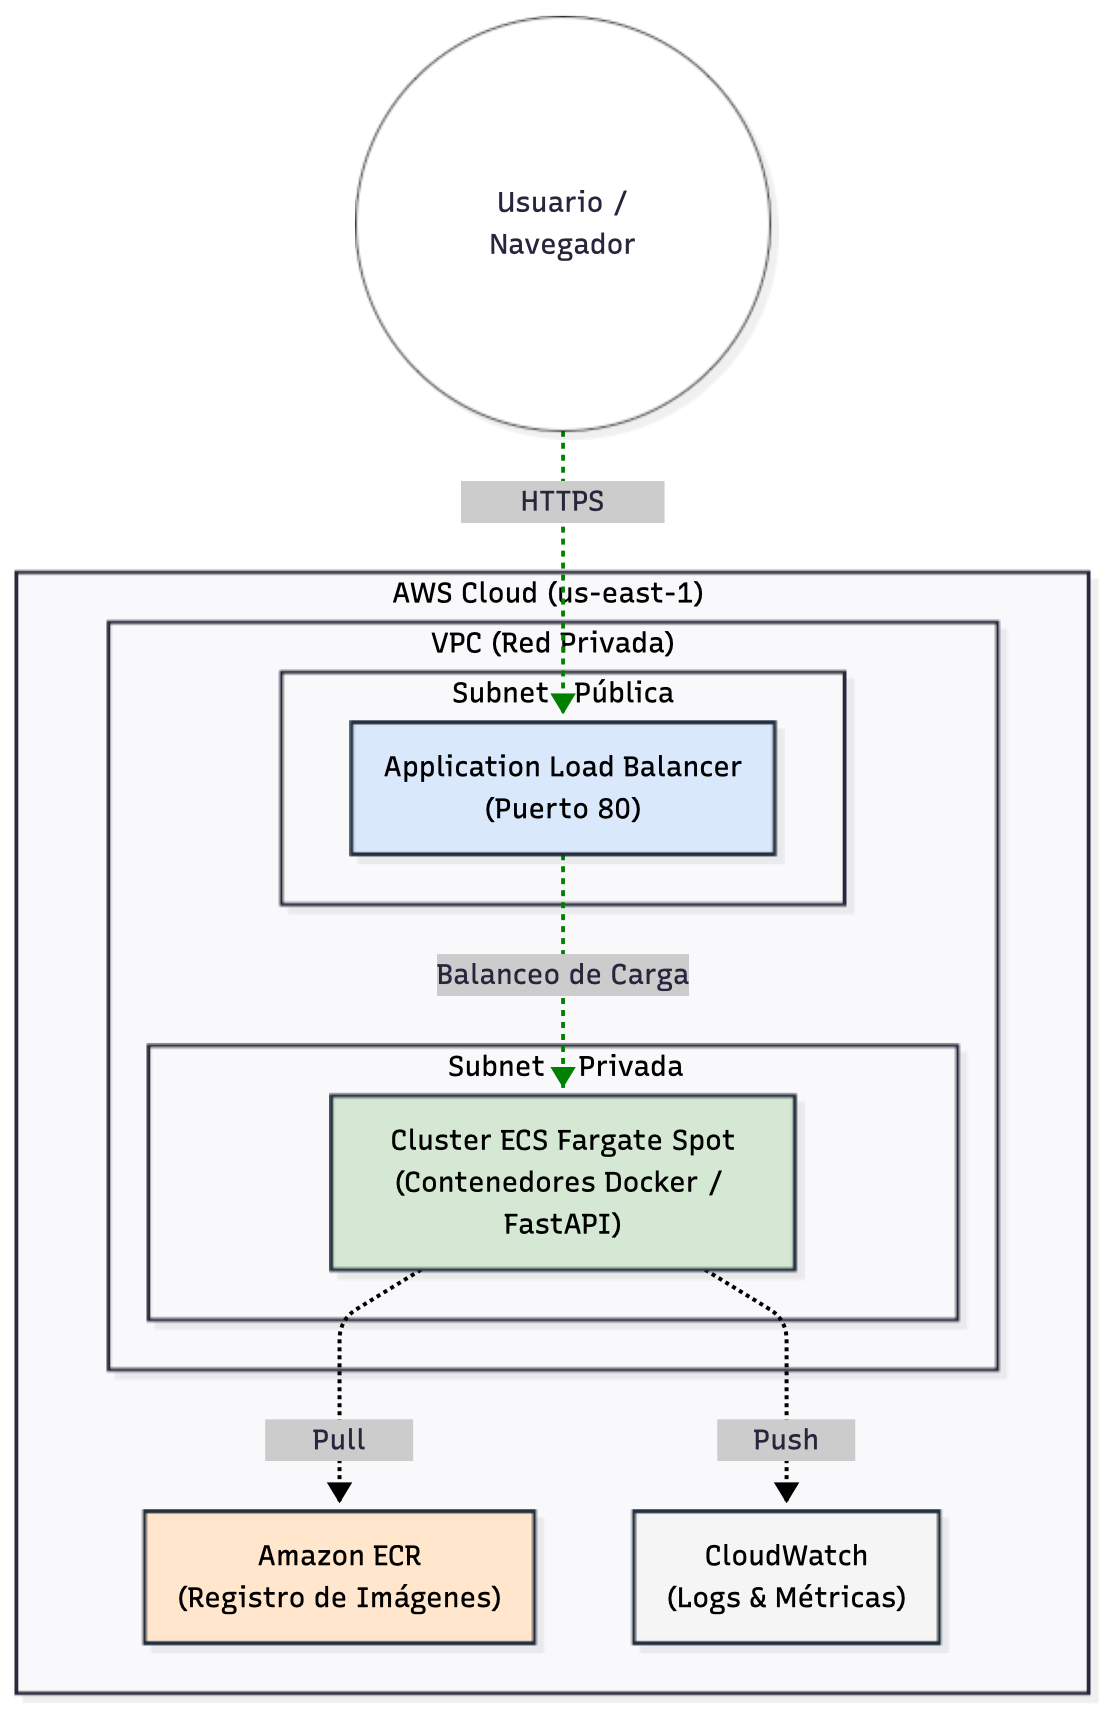
\includegraphics[width=0.4\textwidth]{static/img/arquitectura_despliegue.png}
%     \caption{Arquitectura de despliegue de la solución en la nube.}
    \caption{Cloud deployment architecture of the solution.}
    \label{fig:deployment_arch}
\end{figure}


% \section{Resultados y evaluación}
%
% Se presenta una evaluación del rendimiento de tres variantes de RF-DETR (Nano, Small, Large) en comparación con HerdNet, el modelo de referencia establecido en la literatura para la detección de fauna en manadas densas. Los resultados se organizan en subsecciones que analizan: (1) el rendimiento cuantitativo general, (2) la precisión por especie y el impacto en clases minoritarias, (3) el efecto del HNM, y (4) la eficiencia computacional y viabilidad práctica de los modelos.

\section{Results and Evaluation}

An evaluation of the performance of three RF-DETR variants (Nano, Small, Large) is presented in comparison with HerdNet, the reference model established in the literature for wildlife detection in dense herds. The results are organized in subsections that analyze: (1) overall quantitative performance, (2) per-species accuracy and impact on minority classes, (3) the effect of HNM, and (4) computational efficiency and practical viability of the models.

% \subsection{Rendimiento Cuantitativo Comparativo}
%
% \subsubsection{Métricas}
%
% Para evaluar los modelos tomamos las métricas de referencia de \textit{HerdNet}: precisión, recall y f1, en sus variantes por clase y binaria, en esta última una confusión entre especies de animales no se penaliza, ya que solo se tiene en cuenta la detección de un animal, independiente de su especie. De esta forma definimos las métricas como sigue:
%
% \begin{itemize}
%     \item \textbf{Verdadero positivo (VP)}: una detección es un verdadero positivo si su centro está cerca de un animal de la fuente de la verdad por no más de \textbf{20px} y la clase está correctamente clasificada (métricas por clase).
%
%     \item \textbf{Falso negativo (FN)}: se considera un falso negativo si para una anotación de la fuente de la verdad no existe una detección en predicciones que esté a menos de \textbf{20px}. Para métricas por clase, la clase debe ser igual en la fuente de la verdad y detecciones.
%
%     \item \textbf{Falso positivo (FP)}: se considera un falso positivo toda detección que no esté cerca de ninguna etiqueta de la fuente de la verdad (menos de \textbf{20px} de distancia desde el centro) cuya clase coincida (para el caso de métricas por clase).
% \end{itemize}
%
% \noindent Las métricas se definen como:

\subsection{Comparative Quantitative Performance}

\subsubsection{Metrics}

To evaluate the models, we adopt the reference metrics from \textit{HerdNet}: precision, recall, and f1, in their per-class and binary variants. In the latter, confusion between animal species is not penalized, as only the detection of an animal is considered, regardless of its species. Thus, we define the metrics as follows:

\begin{itemize}
    \item \textbf{True positive (TP)}: a detection is a true positive if its center is close to an animal from the ground truth by no more than \textbf{20px} and the class is correctly classified (per-class metrics).

    \item \textbf{False negative (FN)}: it is considered a false negative if for a ground truth annotation there is no detection in predictions within \textbf{20px}. For per-class metrics, the class must be equal in ground truth and detections.

    \item \textbf{False positive (FP)}: every detection that is not close to any ground truth label (less than \textbf{20px} distance from the center) whose class matches (for the case of per-class metrics) is considered a false positive.
\end{itemize}

\noindent The metrics are defined as:

% \[
% \text{Precisión (P)} = \frac{VP}{VP + FP}
% \]
%
% \[
% \text{Recall (R)} = \frac{VP}{VP + FN}
% \]
%
% \[
% \text{Puntaje F1} = 2 \cdot \frac{\text{Precisión} \cdot \text{Recall}}{\text{Precisión} + \text{Recall}}
% \]
%
% \[
% \text{MAE} = \frac{1}{I} \sum_{i=1}^{I} \left| \hat{n}_i - n_i \right|
% \]
%
% \[
% \text{RMSE} = \sqrt{\frac{1}{I} \sum_{i=1}^{I} \left( \hat{n}_i - n_i \right)^2}
% \]

\[
\text{Precision (P)} = \frac{TP}{TP + FP}
\]

\[
\text{Recall (R)} = \frac{TP}{TP + FN}
\]

\[
\text{F1 Score} = 2 \cdot \frac{\text{Precision} \cdot \text{Recall}}{\text{Precision} + \text{Recall}}
\]

\[
\text{MAE} = \frac{1}{I} \sum_{i=1}^{I} \left| \hat{n}_i - n_i \right|
\]

\[
\text{RMSE} = \sqrt{\frac{1}{I} \sum_{i=1}^{I} \left( \hat{n}_i - n_i \right)^2}
\]

% \subsubsection{Métricas globales de rendimiento en el conjunto de prueba}
% La Tabla \ref{tab:overall_metrics} presenta las métricas globales de rendimiento para los cuatro modelos evaluados en sus dos fases de entrenamiento. Esta comparación permite analizar tanto el rendimiento final como el impacto del HNM en cada arquitectura. Los resultados de Fase 2 demuestran mejoras consistentes de las variantes RF-DETR sobre el baseline HerdNet en las métricas críticas de precisión y conteo.
%
% \begin{table}[ht]
% \centering
% \caption{Métricas globales de rendimiento en el conjunto de prueba: comparación Fase 1 (entrenamiento inicial) vs Fase 2 (con Hard Negative Mining).}
% \label{tab:overall_metrics}
% \resizebox{\columnwidth}{!}{%
% \begin{tabular}{llccccc}
% \hline
% \textbf{Modelo} & \textbf{Fase} & \textbf{Precision} & \textbf{Recall} & \textbf{F1-Score} & \textbf{MAE} & \textbf{RMSE} \\ \hline
% \multirow{2}{*}{HerdNet}
% & Fase 1 & 0.6154 & 0.8673 & 0.7200 & 4.3450 & 9.8746 \\
% & Fase 2 & 0.8229 & 0.8425 & 0.8326 & 1.8953 & 3.6700 \\ \hline
% \multirow{2}{*}{RF-DETR nano}
% & Fase 1 & 0.5023 & 0.9378 & 0.6542 & 7.7403 & 10.9341 \\
% & Fase 2 & 0.8161 & 0.6407 & 0.7178 & 3.7287 & 6.8957 \\ \hline
% \multirow{2}{*}{RF-DETR small}
% & Fase 1 & 0.2615 & 0.9517 & 0.4103 & 23.5310 & 32.0026 \\
% & Fase 2 & \textbf{0.9385} & 0.8691 & \textbf{0.9024} & \textbf{1.1473} & \textbf{2.4112} \\ \hline
% \multirow{2}{*}{RF-DETR large}
% & Fase 1 & 0.6133 & 0.9230 & 0.7369 & 4.8643 & 7.5742 \\
% & Fase 2 & 0.8893 & \textbf{0.8839} & 0.8866 & 1.2248 & 3.0966 \\ \hline
% \end{tabular}%
% }
% \end{table}

\subsubsection{Overall Performance Metrics on the Test Set}
Table \ref{tab:overall_metrics} presents the overall performance metrics for the four evaluated models in their two training phases. This comparison allows analyzing both the final performance and the impact of HNM on each architecture. Phase 2 results demonstrate consistent improvements of RF-DETR variants over the baseline HerdNet in critical metrics of precision and counting.

\begin{table}[ht]
\centering
\caption{Overall performance metrics on the test set: comparison Phase 1 (initial training) vs Phase 2 (with Hard Negative Mining).}
\label{tab:overall_metrics}
\resizebox{\columnwidth}{!}{%
\begin{tabular}{llccccc}
\hline
\textbf{Model} & \textbf{Phase} & \textbf{Precision} & \textbf{Recall} & \textbf{F1-Score} & \textbf{MAE} & \textbf{RMSE} \\ \hline
\multirow{2}{*}{HerdNet}
& Phase 1 & 0.6154 & 0.8673 & 0.7200 & 4.3450 & 9.8746 \\
& Phase 2 & 0.8229 & 0.8425 & 0.8326 & 1.8953 & 3.6700 \\ \hline
\multirow{2}{*}{RF-DETR nano}
& Phase 1 & 0.5023 & 0.9378 & 0.6542 & 7.7403 & 10.9341 \\
& Phase 2 & 0.8161 & 0.6407 & 0.7178 & 3.7287 & 6.8957 \\ \hline
\multirow{2}{*}{RF-DETR small}
& Phase 1 & 0.2615 & 0.9517 & 0.4103 & 23.5310 & 32.0026 \\
& Phase 2 & \textbf{0.9385} & 0.8691 & \textbf{0.9024} & \textbf{1.1473} & \textbf{2.4112} \\ \hline
\multirow{2}{*}{RF-DETR large}
& Phase 1 & 0.6133 & 0.9230 & 0.7369 & 4.8643 & 7.5742 \\
& Phase 2 & 0.8893 & \textbf{0.8839} & 0.8866 & 1.2248 & 3.0966 \\ \hline
\end{tabular}%
}
\end{table}

% \textbf{RF-DETR small} se posiciona como el modelo de mejor desempeño global, alcanzando un F1-Score de 90.24\%, lo que representa una mejora del \textbf{8.37\%} sobre HerdNet (83.26\%). Esta mejora se debe principalmente a un incremento sustancial en precisión (93.85\% vs 82.29\%), indicando una reducción significativa de falsos positivos. Simultáneamente, el recall se mantuvo competitivo (86.91\% vs 84.25\%), demostrando que la eliminación del NMS no compromete la capacidad de recuperación de individuos.
%
% El análisis de las métricas de error de conteo revela mejoras aún más pronunciadas. RF-DETR small redujo el MAE en un \textbf{39.47\%} (de 1.90 a 1.15) y el RMSE en un \textbf{34.29\%} (de 3.67 a 2.41) en comparación con HerdNet Fase 2. Estas reducciones son críticas para aplicaciones de conservación, donde el conteo preciso de poblaciones es fundamental para la toma de decisiones de gestión.
%
% \textbf{RF-DETR large}, con un F1-Score de 88.66\%, también superó significativamente a HerdNet (+6.48\%), alcanzando el mejor recall de 88.39\%. Sin embargo, \textbf{RF-DETR nano} presenta un rendimiento considerablemente inferior (F1=71.78\%), especialmente en recall (64.07\%), lo que sugiere que la arquitectura nano carece de la capacidad expresiva necesaria para capturar la complejidad de escenarios multiespecie con alta oclusión.
%
% Un patrón crítico emerge al comparar ambas fases de entrenamiento: todos los modelos en Fase 1 priorizaban recall sobre precisión, resultando en F1-Scores subóptimos debido a la generación excesiva de falsos positivos. RF-DETR small mostró el comportamiento más extremo, alcanzando un recall de 95.17\% en Fase 1 pero con una precisión de apenas 26.15\%, generando un MAE de 23.53. El refinamiento mediante HNM en Fase 2 corrigió este desbalance sistemáticamente, mejorando la precisión de todos los modelos mientras mantenía niveles aceptables de recall. Este patrón valida la necesidad del entrenamiento en dos fases para aplicaciones donde la precisión de conteo es tan crítica como la capacidad de detección.

\textbf{RF-DETR small} positions itself as the best overall performing model, achieving an F1-Score of 90.24\%, representing an improvement of \textbf{8.37\%} over HerdNet (83.26\%). This improvement is primarily due to a substantial increase in precision (93.85\% vs 82.29\%), indicating a significant reduction of false positives. Simultaneously, recall remained competitive (86.91\% vs 84.25\%), demonstrating that the elimination of NMS does not compromise the ability to recover individuals.

The analysis of counting error metrics reveals even more pronounced improvements. RF-DETR small reduced MAE by \textbf{39.47\%} (from 1.90 to 1.15) and RMSE by \textbf{34.29\%} (from 3.67 to 2.41) compared to HerdNet Phase 2. These reductions are critical for conservation applications, where accurate population counting is fundamental for management decision-making.

\textbf{RF-DETR large}, with an F1-Score of 88.66\%, also significantly outperformed HerdNet (+6.48\%), achieving the best recall of 88.39\%. However, \textbf{RF-DETR nano} presents considerably inferior performance (F1=71.78\%), especially in recall (64.07\%), suggesting that the nano architecture lacks the expressive capacity necessary to capture the complexity of multi-species scenarios with high occlusion.

A critical pattern emerges when comparing both training phases: all models in Phase 1 prioritized recall over precision, resulting in suboptimal F1-Scores due to excessive generation of false positives. RF-DETR small showed the most extreme behavior, achieving a recall of 95.17\% in Phase 1 but with a precision of only 26.15\%, generating a MAE of 23.53. Refinement through HNM in Phase 2 systematically corrected this imbalance, improving the precision of all models while maintaining acceptable recall levels. This pattern validates the need for two-phase training for applications where counting precision is as critical as detection capability.

% \subsection{Análisis por Especie y Clases Minoritarias}
%
% La Figura \ref{fig:f1_per_class} presenta el F1-Score desagregado por especie, revelando patrones diferenciados de rendimiento que validan una de las hipótesis centrales de este trabajo: los Transformers mejoran la discriminación en especies minoritarias.
%
% \begin{figure*}[t]
%     \centering
%     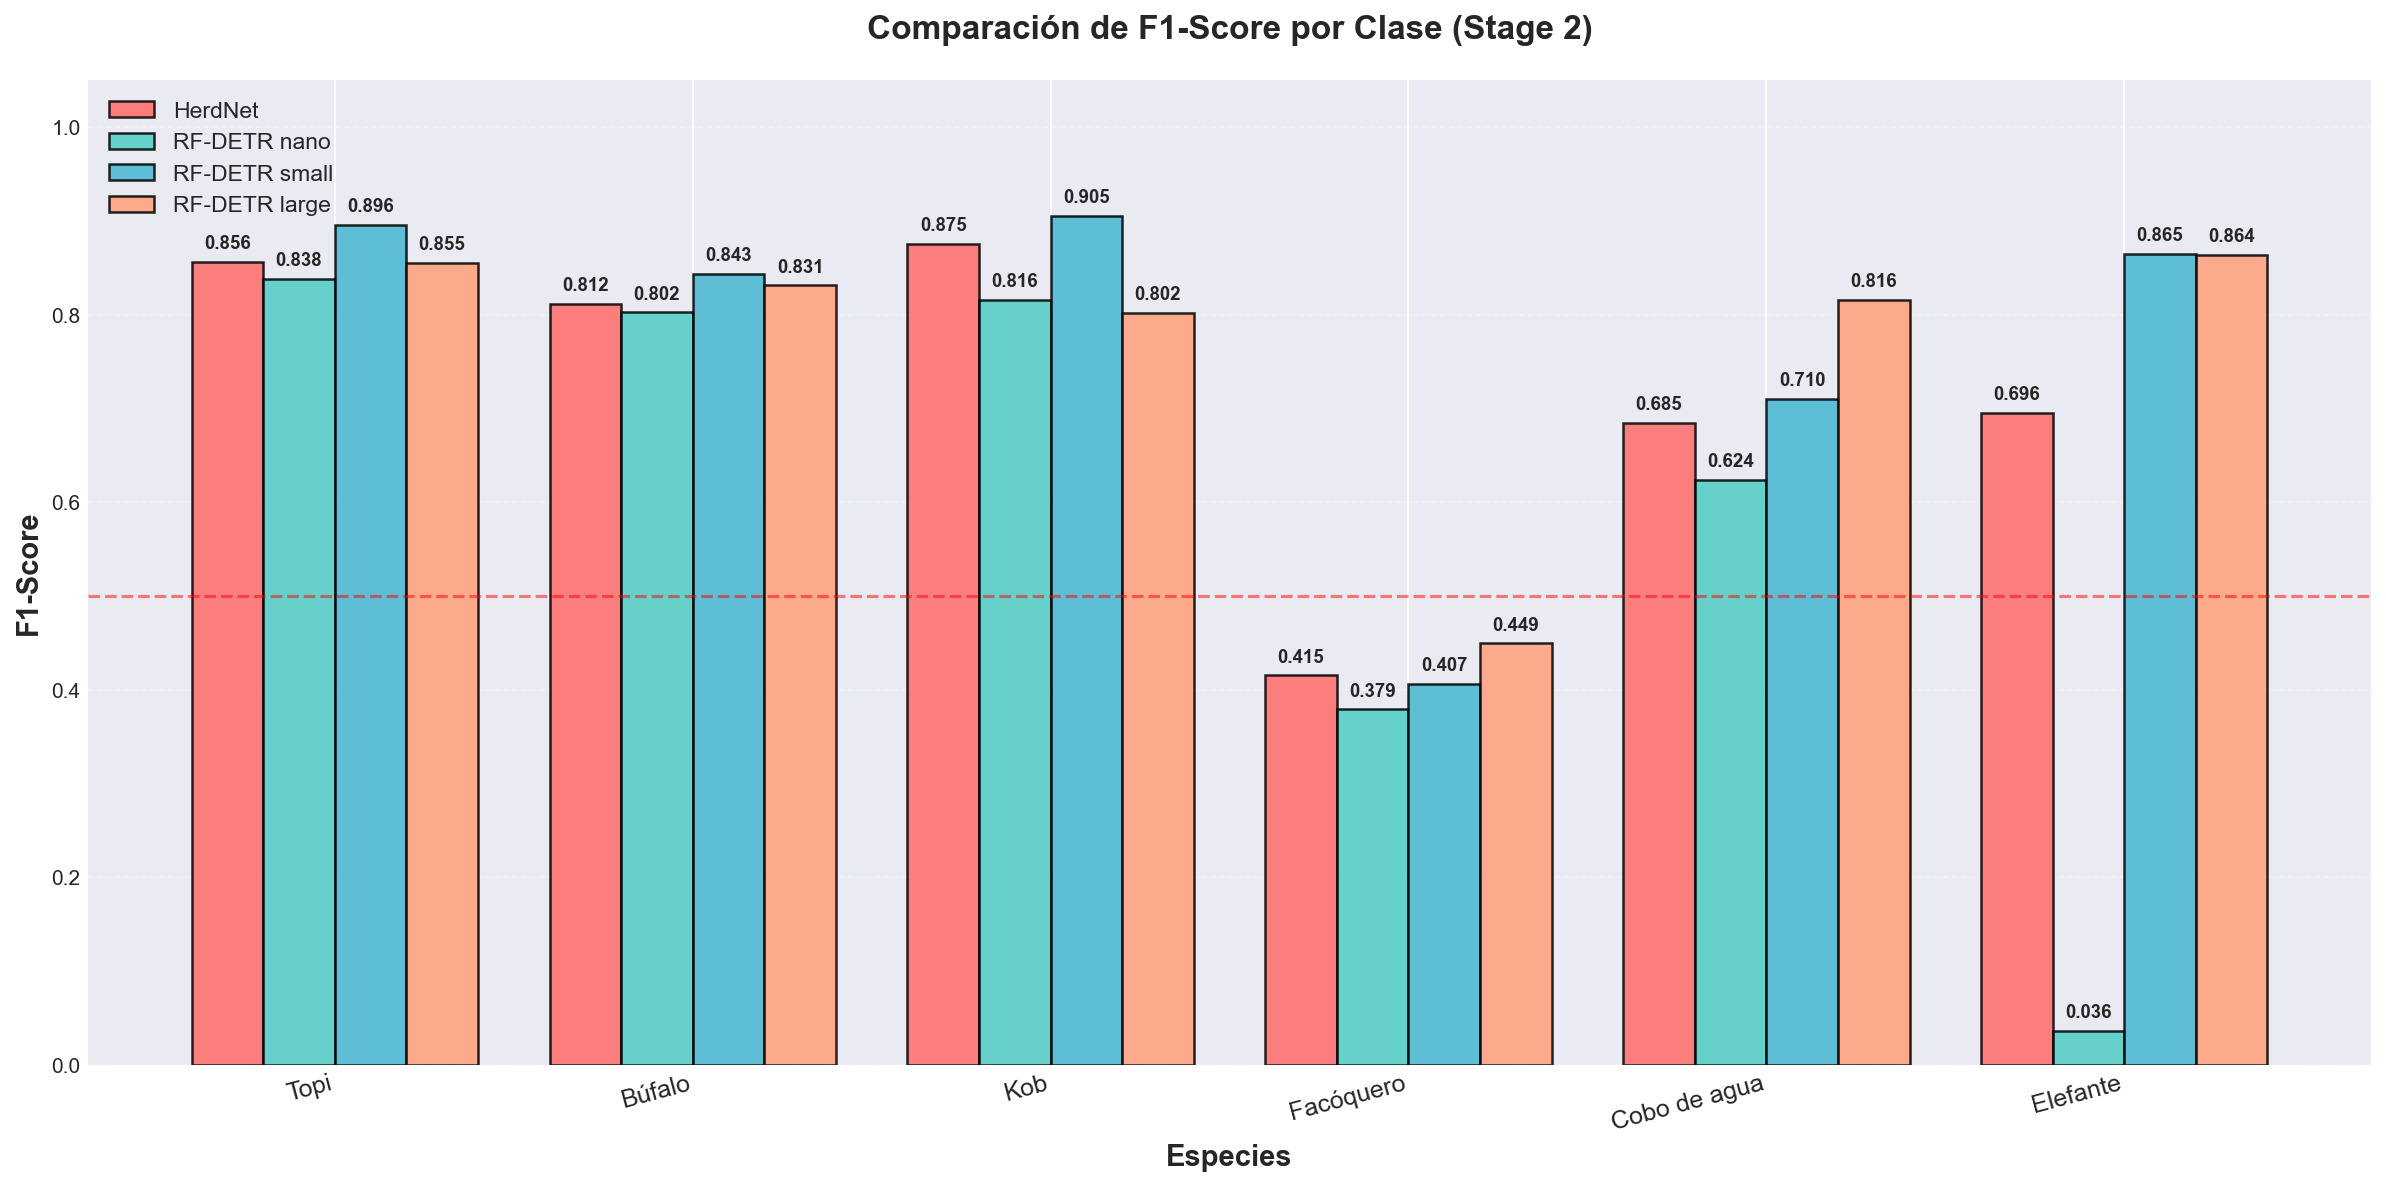
\includegraphics[width=\textwidth]{static/img/f1_score_por_clase_stage2.png}
%     \caption{F1-Score por especie para todos los modelos en Fase 2.}
%     \label{fig:f1_per_class}
% \end{figure*}
%
% Los resultados más destacados se observan en las dos especies minoritarias del dataset:
%
% \textbf{Cobo de agua:} RF-DETR large alcanzó un F1-Score de \textbf{0.816}, representando una mejora del \textbf{19.1\%} sobre HerdNet (0.685). Esta mejora se atribuye a un recall excepcional de 86.1\% y una precisión de 77.5\%, indicando que el modelo captura exitosamente la mayoría de los individuos de esta especie extremadamente subrepresentada (241 individuos en total, apenas el 2.4\% del dataset).
%
% \textbf{Facóquero:} Aunque la mejora fue más modesta, RF-DETR large alcanzó un F1-Score de 0.449 versus 0.415 de HerdNet (mejora del 8.2\%). Sin embargo, la precisión mejoró significativamente (0.484 vs 0.388), reduciendo los falsos positivos en un 24.7\%.
%
% Para especies mayoritarias como Elefante y Kob, el rendimiento tuvo mejoras incrementales de RF-DETR. Lo que indica que no se sacrifica el rendimiento en clases bien representadas mientras se mejora sustancialmente la detección de especies minoritarias, un equilibrio crítico para aplicaciones reales de monitoreo multiespecie.

\subsection{Per-Species Analysis and Minority Classes}

Figure \ref{fig:f1_per_class} presents the F1-Score disaggregated by species, revealing differentiated performance patterns that validate one of the central hypotheses of this work: Transformers improve discrimination in minority species.

\begin{figure*}[t]
    \centering
    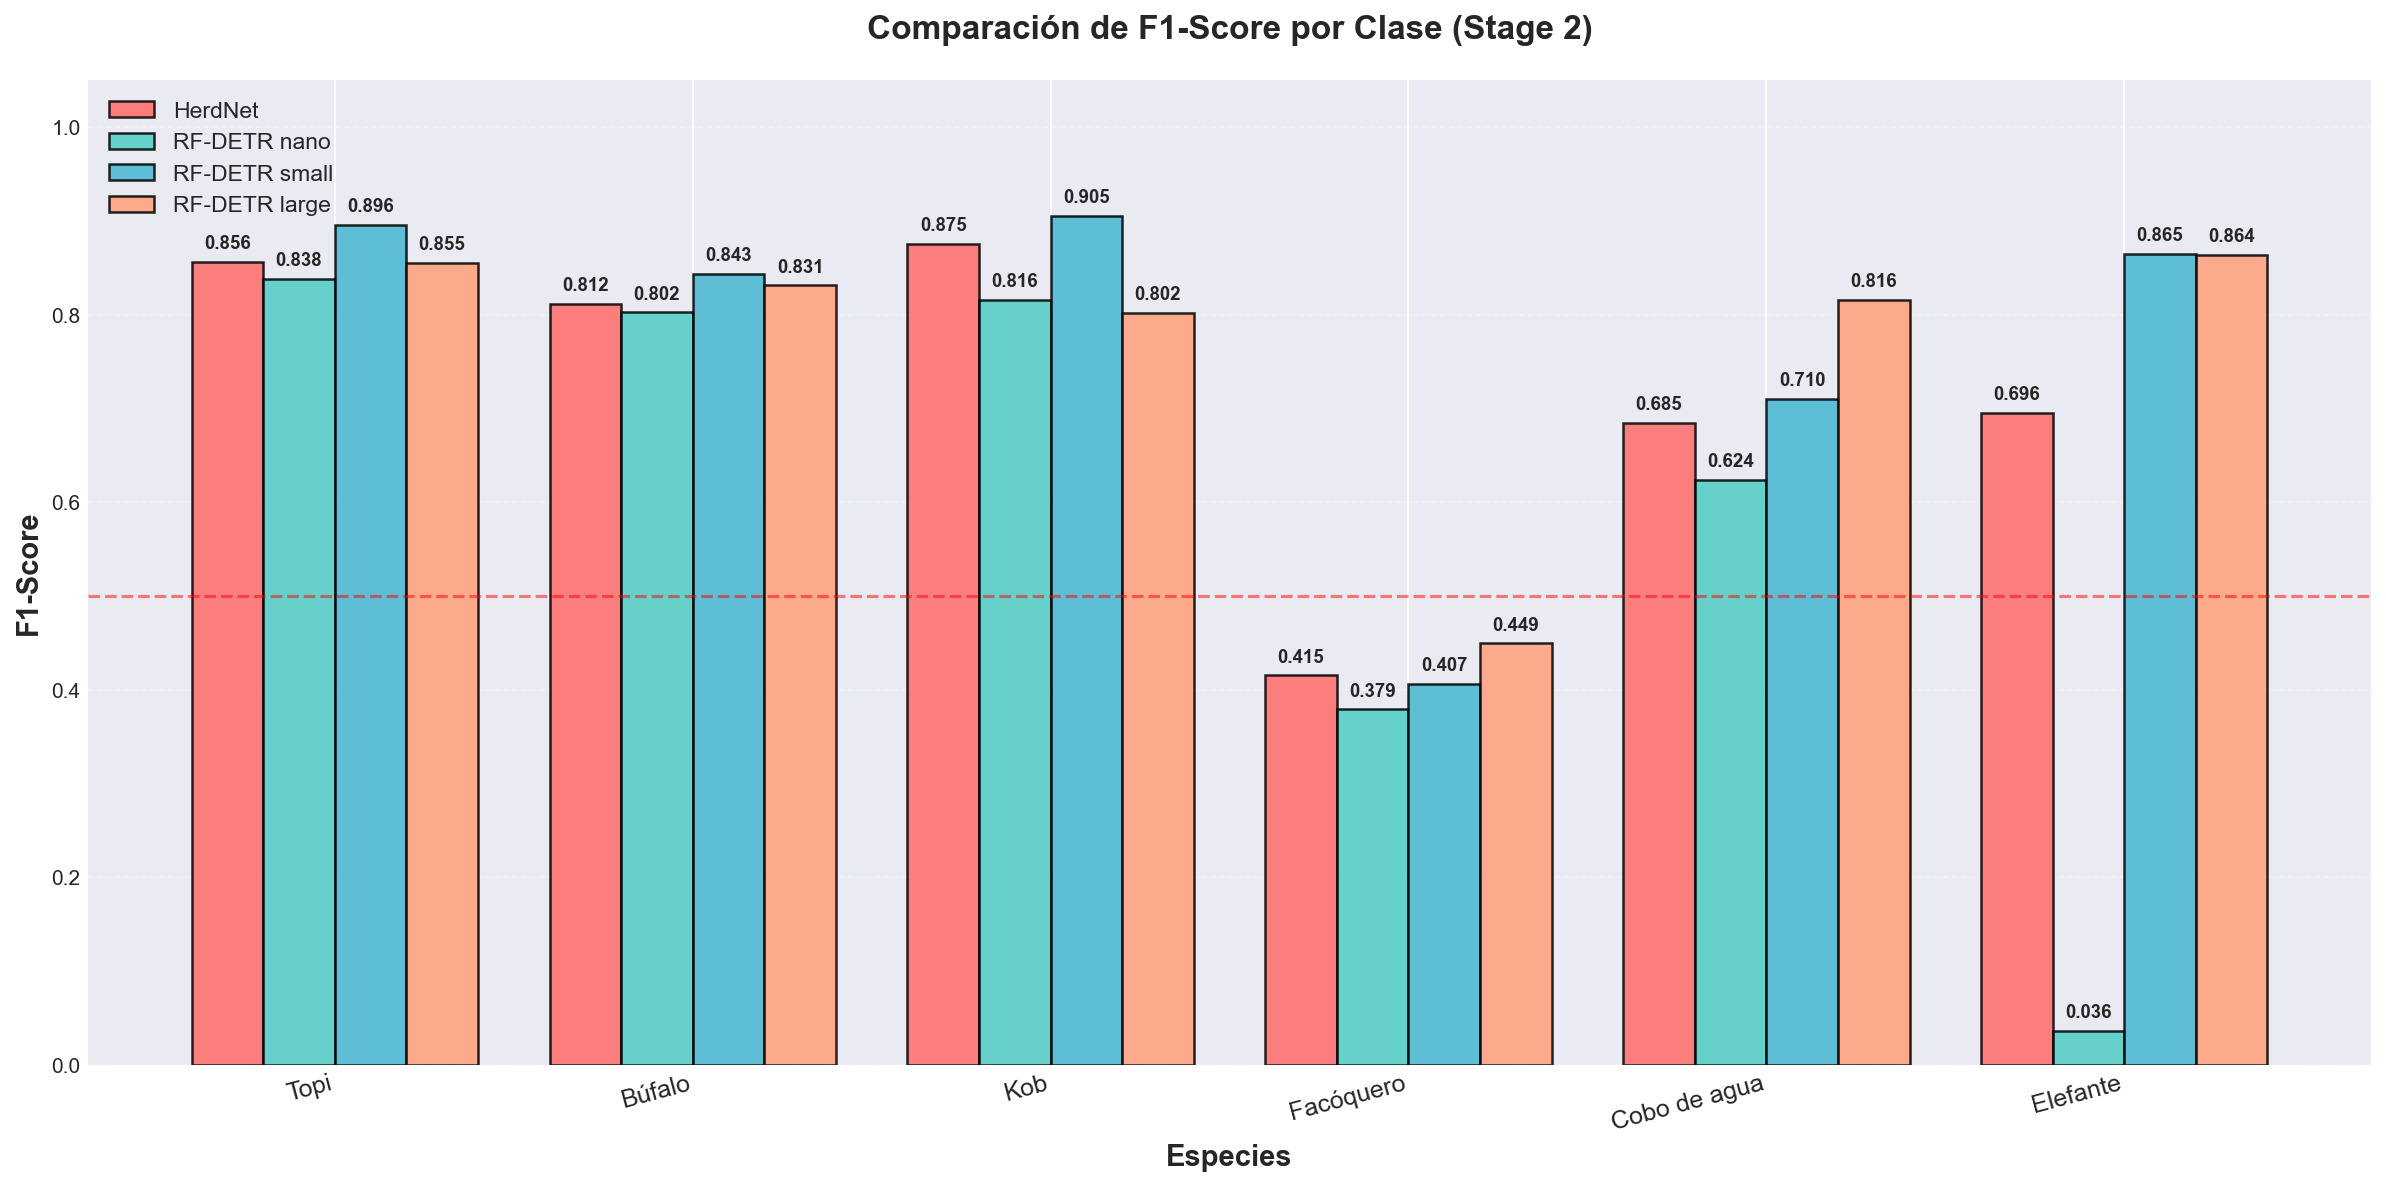
\includegraphics[width=\textwidth]{static/img/f1_score_por_clase_stage2.png}
    \caption{F1-Score per species for all models in Phase 2.}
    \label{fig:f1_per_class}
\end{figure*}

The most outstanding results are observed in the two minority species of the dataset:

\textbf{Waterbuck:} RF-DETR large achieved an F1-Score of \textbf{0.816}, representing an improvement of \textbf{19.1\%} over HerdNet (0.685). This improvement is attributed to an exceptional recall of 86.1\% and a precision of 77.5\%, indicating that the model successfully captures most individuals of this extremely underrepresented species (241 individuals in total, barely 2.4\% of the dataset).

\textbf{Warthog:} Although the improvement was more modest, RF-DETR large achieved an F1-Score of 0.449 versus 0.415 for HerdNet (8.2\% improvement). However, precision improved significantly (0.484 vs 0.388), reducing false positives by 24.7\%.

For majority species such as Elephant and Kob, performance had incremental improvements from RF-DETR. This indicates that performance on well-represented classes is not sacrificed while substantially improving detection of minority species, a critical balance for real multi-species monitoring applications.

% \subsection{Impacto del Hard Negative Mining}
%
% Como se observa en la Tabla \ref{tab:overall_metrics}, la estrategia de dos fases con HNM fue fundamental para alcanzar el rendimiento final reportado. La comparación entre Fase 1 y Fase 2 revela mejoras diferenciadas según la arquitectura, reflejando distintos niveles de susceptibilidad a la generación de falsos positivos durante el entrenamiento inicial.
%
% \textbf{RF-DETR small} mostró el impacto más significativo del HNM, con un incremento en precisión de 0.26 a 0.94 (mejora relativa del \textbf{258.9\%}), lo que indica que el modelo sin refinamiento presentaba una alta tasa de falsos positivos en patrones ambiguos. El F1-Score pasó de 0.41 a 0.90 (mejora del \textbf{119.9\%}), transformándolo de un modelo con rendimiento limitado a la mejor solución del estudio. Este comportamiento sugiere que la arquitectura small, con su mayor capacidad expresiva, es particularmente susceptible a generar falsos positivos en fondos complejos cuando se entrena sin ejemplos negativos difíciles.
%
% En contraste, \textbf{HerdNet} y \textbf{RF-DETR large} mostraron mejoras más moderadas pero consistentes. HerdNet incrementó su precisión en +33.7\% (de 0.62 a 0.82) y su F1-Score en +15.6\% (de 0.72 a 0.83), mientras que RF-DETR large mejoró +45.0\% en precisión (de 0.61 a 0.89) y +20.3\% en F1-Score (de 0.74 a 0.89). Estas mejoras más moderadas indican que ambas arquitecturas poseían cierta robustez intrínseca contra falsos positivos desde la Fase 1, requiriendo un refinamiento menos agresivo. \textbf{RF-DETR nano}, por su parte, mejoró su precisión en +62.5\% (de 0.50 a 0.82), aunque su F1-Score final (0.72) permaneció por debajo del baseline, confirmando las limitaciones arquitectónicas de la variante más compacta.
%
% La incorporación sistemática de estos ejemplos difíciles en la Fase 2 permitió a los modelos desarrollar representaciones más discriminativas, aprendiendo a distinguir características texturales y contextuales sutiles que separan animales reales de elementos de background visualmente similares.

\subsection{Impact of Hard Negative Mining}

As observed in Table \ref{tab:overall_metrics}, the two-phase strategy with HNM was fundamental to achieve the final reported performance. The comparison between Phase 1 and Phase 2 reveals differentiated improvements according to architecture, reflecting different levels of susceptibility to false positive generation during initial training.

\textbf{RF-DETR small} showed the most significant impact from HNM, with an increase in precision from 0.26 to 0.94 (relative improvement of \textbf{258.9\%}), indicating that the model without refinement exhibited a high rate of false positives on ambiguous patterns. The F1-Score went from 0.41 to 0.90 (improvement of \textbf{119.9\%}), transforming it from a model with limited performance to the best solution of the study. This behavior suggests that the small architecture, with its greater expressive capacity, is particularly susceptible to generating false positives on complex backgrounds when trained without hard negative examples.

In contrast, \textbf{HerdNet} and \textbf{RF-DETR large} showed more moderate but consistent improvements. HerdNet increased its precision by +33.7\% (from 0.62 to 0.82) and its F1-Score by +15.6\% (from 0.72 to 0.83), while RF-DETR large improved +45.0\% in precision (from 0.61 to 0.89) and +20.3\% in F1-Score (from 0.74 to 0.89). These more moderate improvements indicate that both architectures possessed certain intrinsic robustness against false positives from Phase 1, requiring less aggressive refinement. \textbf{RF-DETR nano}, for its part, improved its precision by +62.5\% (from 0.50 to 0.82), although its final F1-Score (0.72) remained below the baseline, confirming the architectural limitations of the most compact variant.

The systematic incorporation of these hard examples in Phase 2 allowed the models to develop more discriminative representations, learning to distinguish subtle textural and contextual features that separate real animals from visually similar background elements.

% \subsection{Eficiencia Computacional}
%
% La Figura \ref{fig:inference_times} presenta la distribución de latencias de inferencia por imagen medidas en el conjunto de prueba utilizando una GPU NVIDIA A100 (80GB VRAM). Los diagramas de caja revelan tanto la tendencia central como la variabilidad de los tiempos de procesamiento para cada modelo.
%
% \begin{figure}[ht]
%     \centering
%     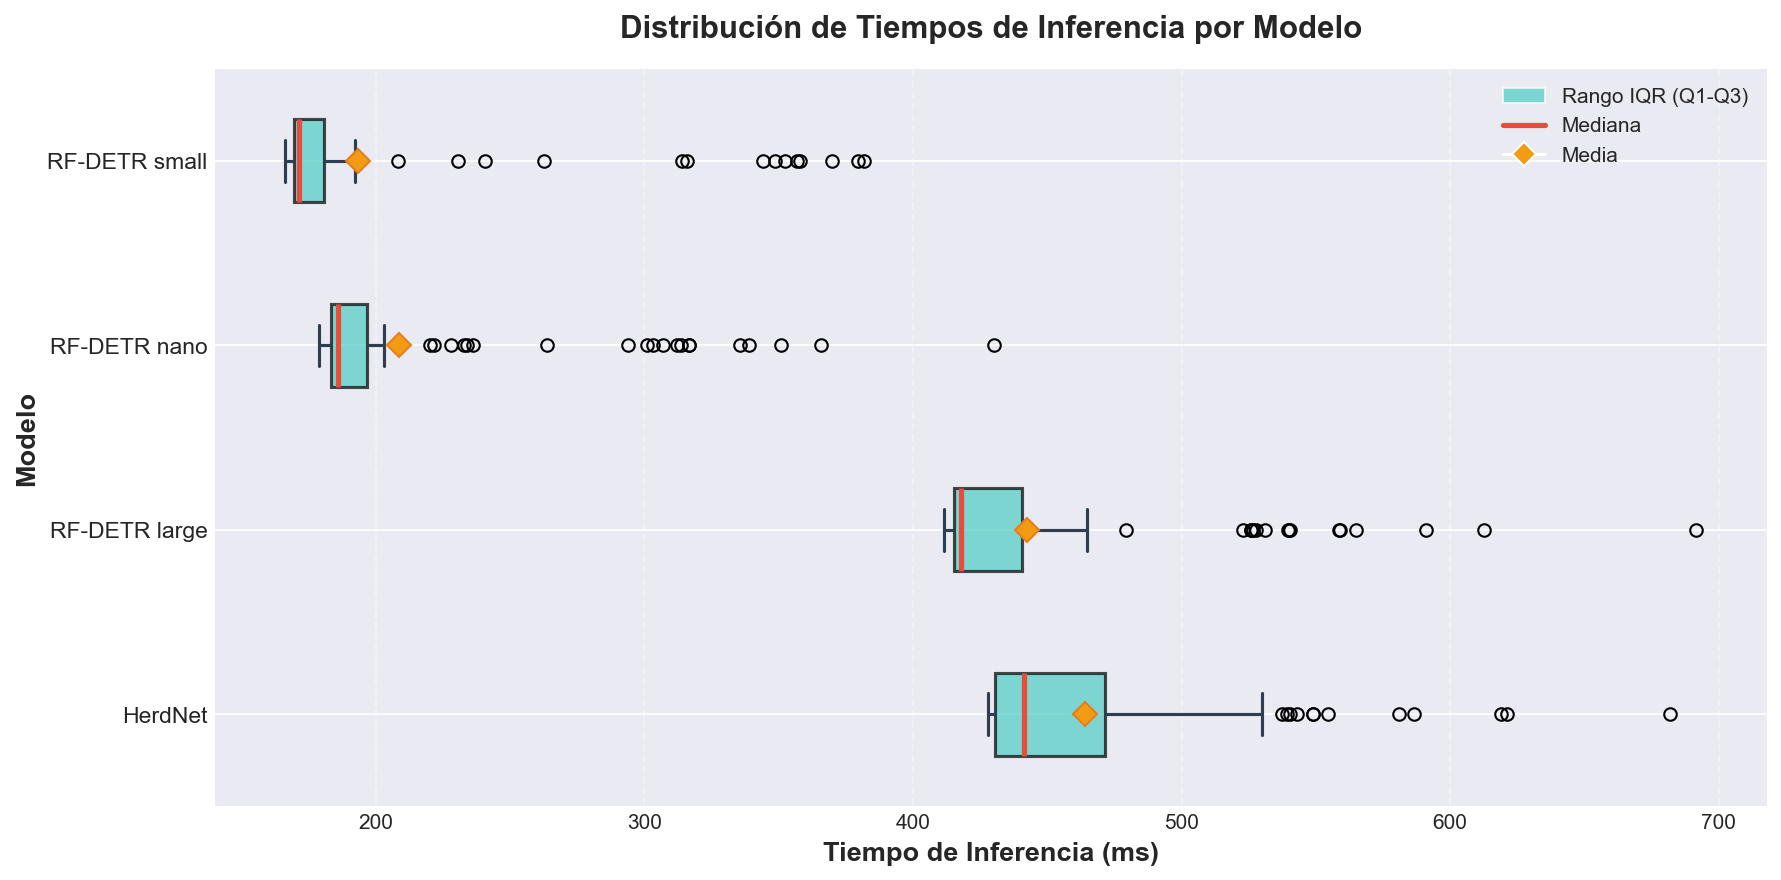
\includegraphics[width=\columnwidth]{static/img/inference_times_boxplot.png}
%     \caption{Distribución de tiempos de inferencia por modelo en conjunto de prueba. La línea roja indica la mediana y el rombo naranja la media.}
%     \label{fig:inference_times}
% \end{figure}
%
% RF-DETR small representa el modelo más eficiente, con una mediana de 171.49 ms y una media de 193.39 ms por imagen, superando incluso a RF-DETR nano (mediana: 186.16 ms, media: 208.53 ms).
%
% HerdNet y RF-DETR large presentan latencias comparables, con medianas de 441.27 ms y 417.88 ms respectivamente, siendo aproximadamente 2.4× más lentos que RF-DETR small. Sin embargo, ambos modelos exhiben mayor variabilidad temporal, como evidencian los outliers presentes en la figura, sugiriendo dependencia en la complejidad de las escenas procesadas.
%
% Para aplicaciones de monitoreo de fauna donde tanto la precisión como el throughput son críticos, RF-DETR small representa la opción óptima al combinar el mejor F1-Score con la menor latencia y mayor consistencia temporal.

\subsection{Computational Efficiency}

Figure \ref{fig:inference_times} presents the distribution of inference latencies per image measured on the test set using an NVIDIA A100 GPU (80GB VRAM). The box plots reveal both the central tendency and variability of processing times for each model.

\begin{figure}[ht]
    \centering
    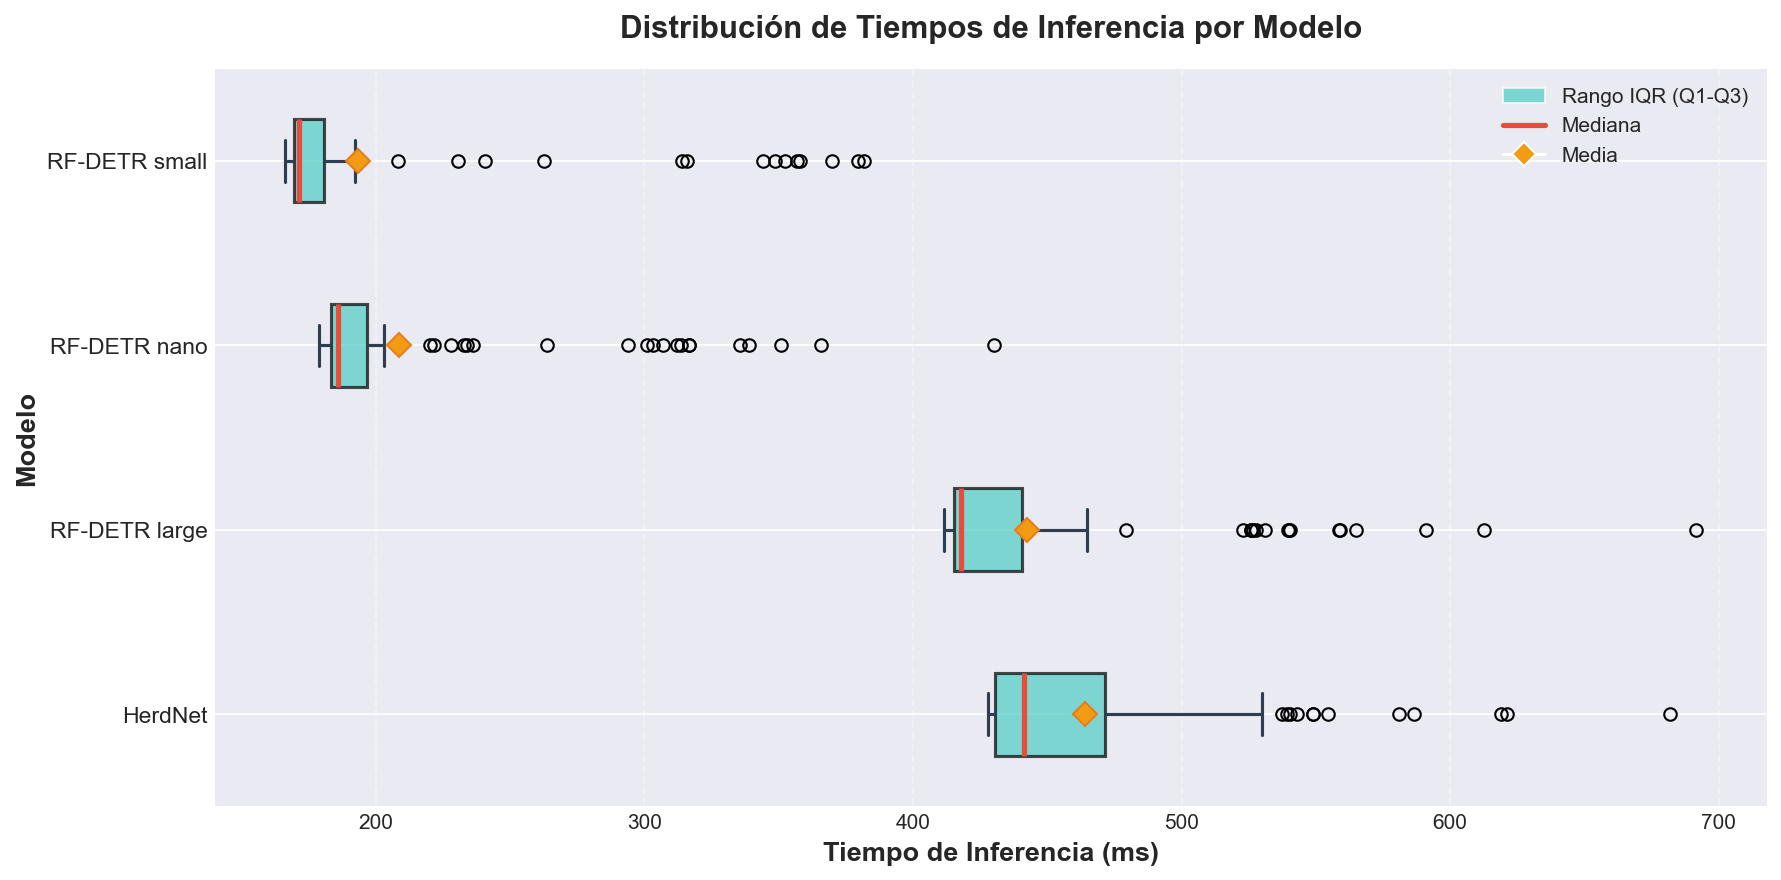
\includegraphics[width=\columnwidth]{static/img/inference_times_boxplot.png}
    \caption{Distribution of inference times per model on the test set. The red line indicates the median and the orange diamond the mean.}
    \label{fig:inference_times}
\end{figure}

RF-DETR small represents the most efficient model, with a median of 171.49 ms and a mean of 193.39 ms per image, even surpassing RF-DETR nano (median: 186.16 ms, mean: 208.53 ms).

HerdNet and RF-DETR large present comparable latencies, with medians of 441.27 ms and 417.88 ms respectively, being approximately 2.4× slower than RF-DETR small. However, both models exhibit greater temporal variability, as evidenced by the outliers present in the figure, suggesting dependence on the complexity of the processed scenes.

For wildlife monitoring applications where both precision and throughput are critical, RF-DETR small represents the optimal option by combining the best F1-Score with the lowest latency and greatest temporal consistency.

% \subsection{Análisis de Matrices de Confusión sobre las detecciones}
%
% La Figura \ref{fig:confusion_matrix} presenta la matriz sobre las detecciones para RF-DETR small, el modelo de mejor desempeño.
%
% \begin{figure}[ht]
%     \centering
%     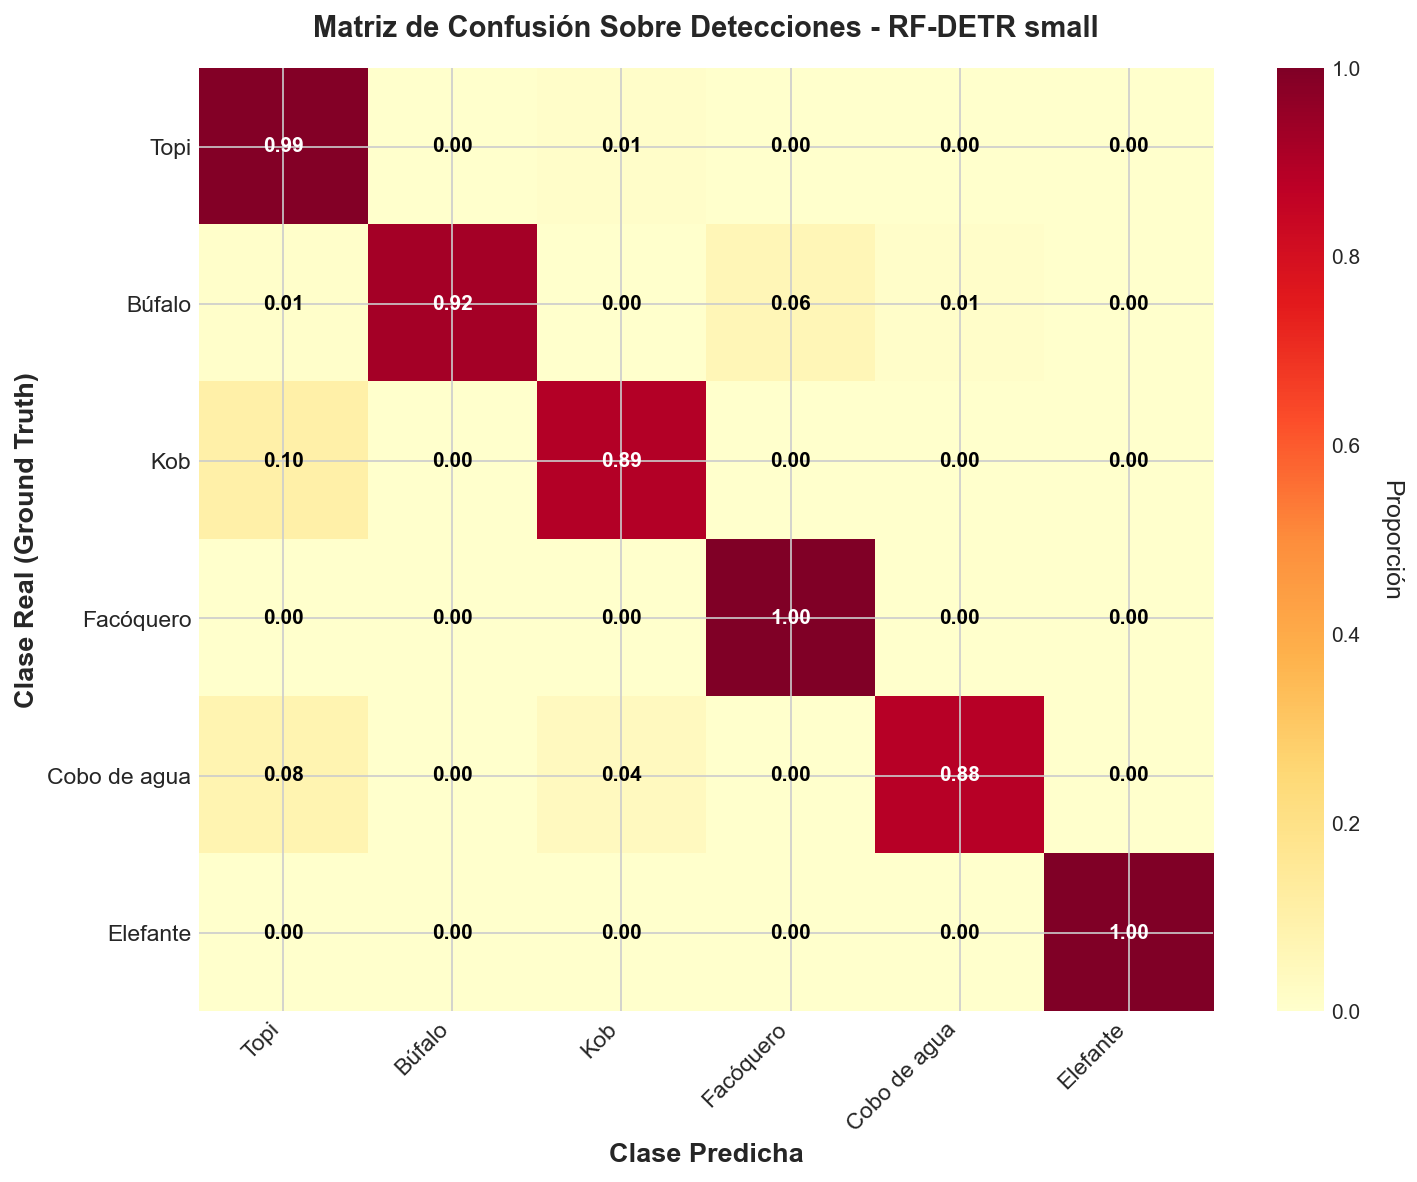
\includegraphics[width=\columnwidth]{static/img/confusion_matrix_rf-detr_small_stage2.png}
%     \caption{Matriz de confusión sobre las detecciones para RF-DETR small (Fase 2).}
%     \label{fig:confusion_matrix}
% \end{figure}
%
% El análisis de la diagonal principal revela una alta eficacia en la clasificación correcta para la mayoría de las especies: Topi (99\%), Búfalo (92\%), Kob (89\%) y Cobo de agua (88\%), destacando un desempeño perfecto (100\%) en las clases Facóquero y Elefante.
%
% Los patrones de confusión interespecífica más relevantes son:
%
% \begin{itemize}
%     \item \textbf{Kob $\rightarrow$ Topi (10\%):} Representa la confusión más significativa del modelo. Es un error unidireccional (la inversa es despreciable), atribuible a la similitud morfológica entre estos antílopes de tamaño medio y pelaje rojizo. El modelo parece identificar mejor los rasgos distintivos del Topi (cuernos curvados y manchas oscuras en las patas) que la morfología más genérica del Kob en ciertas posturas.
%
%     \item \textbf{Cobo de agua $\rightarrow$ Antílopes (12\%):} Esta especie presenta confusiones divididas: un 8\% es clasificado erróneamente como Topi y un 4\% como Kob. Estas confusiones ocurren típicamente cuando el animal está parcialmente ocluido o en ángulos cenitales estrictos donde sus cuernos característicos en forma de lira no son visibles, llevando al modelo a asignarlo a las clases de antílopes mayoritarias.
%
%     \item \textbf{Búfalo $\rightarrow$ Facóquero (6\%):} Se observa una confusión del 6\% de Búfalos clasificados como Facóqueros. Este error, aunque contraintuitivo por la diferencia de tamaño real, puede explicarse por la similitud en la coloración oscura y la textura de la piel en individuos juveniles o en tomas donde la escala relativa es ambigua debido a la altitud de vuelo.
% \end{itemize}

\subsection{Confusion Matrix Analysis on Detections}

Figure \ref{fig:confusion_matrix} presents the confusion matrix on detections for RF-DETR small, the best performing model.

\begin{figure}[ht]
    \centering
    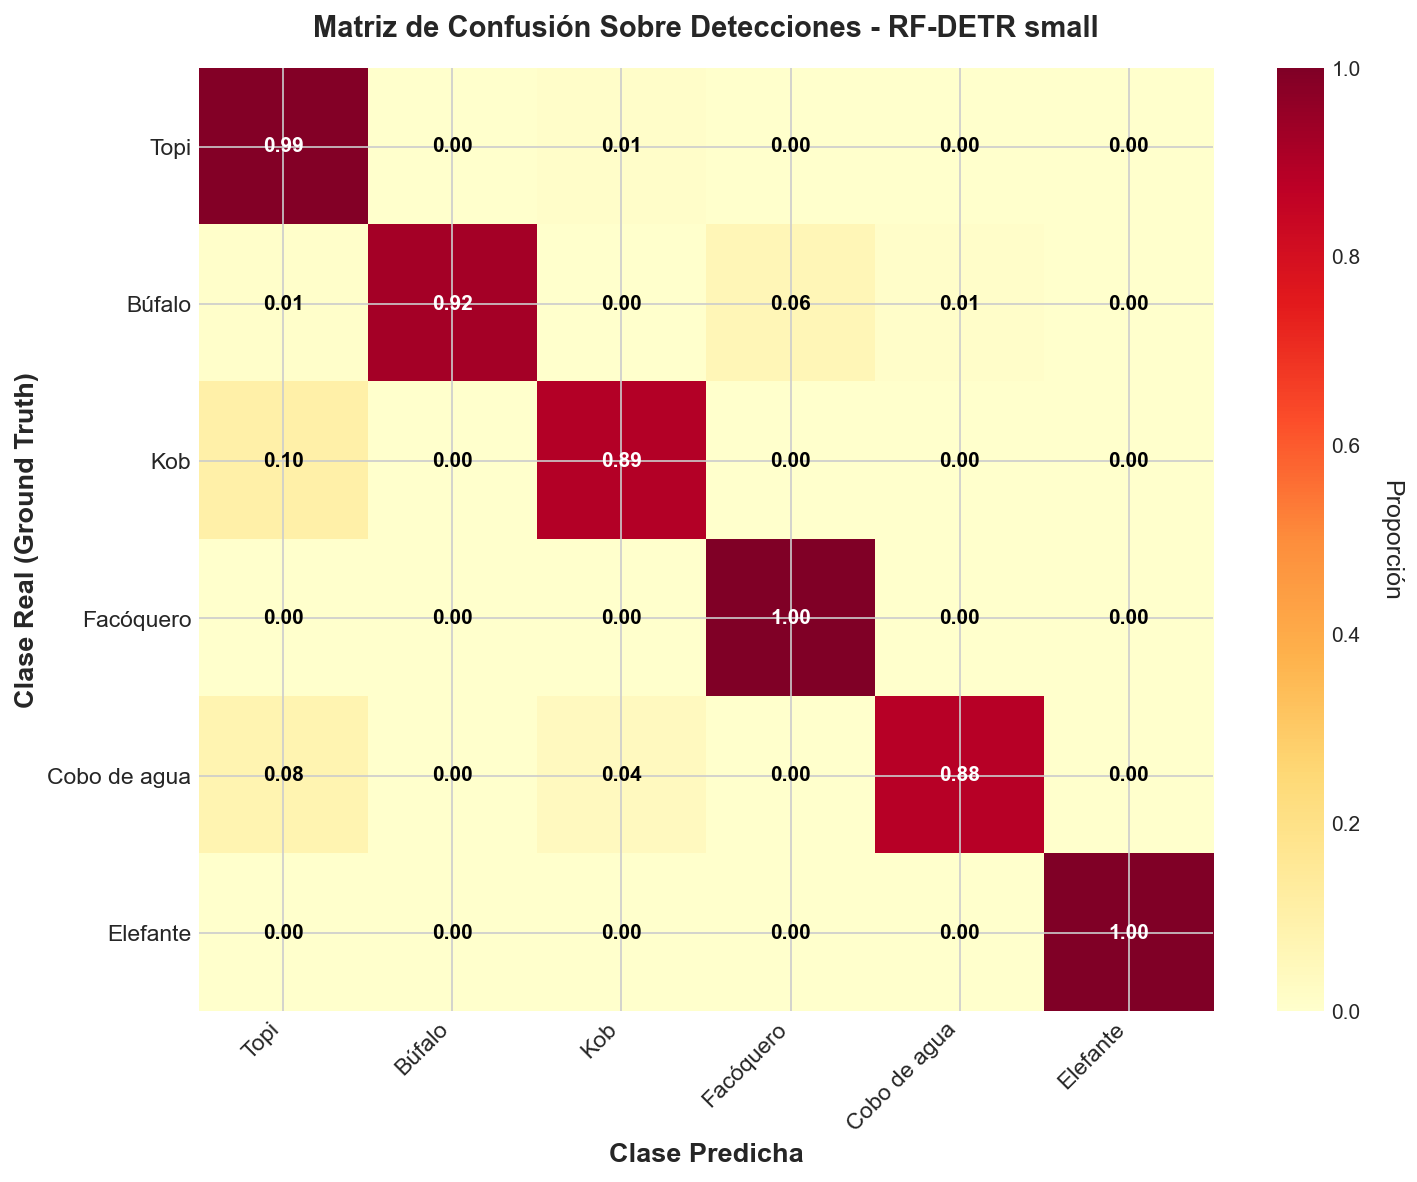
\includegraphics[width=\columnwidth]{static/img/confusion_matrix_rf-detr_small_stage2.png}
    \caption{Confusion matrix on detections for RF-DETR small (Phase 2).}
    \label{fig:confusion_matrix}
\end{figure}

Analysis of the main diagonal reveals high efficacy in correct classification for most species: Topi (99\%), Buffalo (92\%), Kob (89\%), and Waterbuck (88\%), with perfect performance (100\%) standing out in the Warthog and Elephant classes.

The most relevant interspecific confusion patterns are:

\begin{itemize}
    \item \textbf{Kob $\rightarrow$ Topi (10\%):} Represents the model's most significant confusion. It is a unidirectional error (the inverse is negligible), attributable to the morphological similarity between these medium-sized antelopes with reddish fur. The model seems to better identify the distinctive features of Topi (curved horns and dark spots on the legs) than the more generic morphology of Kob in certain postures.

    \item \textbf{Waterbuck $\rightarrow$ Antelopes (12\%):} This species presents divided confusions: 8\% is erroneously classified as Topi and 4\% as Kob. These confusions typically occur when the animal is partially occluded or at strict zenith angles where its characteristic lyre-shaped horns are not visible, leading the model to assign it to the majority antelope classes.

    \item \textbf{Buffalo $\rightarrow$ Warthog (6\%):} A confusion of 6\% of Buffalos classified as Warthogs is observed. This error, although counterintuitive due to the difference in actual size, can be explained by the similarity in dark coloration and skin texture in juvenile individuals or in shots where the relative scale is ambiguous due to flight altitude.
\end{itemize}

% \subsubsection{Interpretación de la Clasificación Perfecta}
% Es notable que especies como el \textbf{Facóquero} y el \textbf{Elefante} alcancen un 100\% en la diagonal de la matriz. Sin embargo, este resultado debe interpretarse con rigor técnico:
%
% \begin{itemize}
%     \item \textbf{Pureza vs. Exhaustividad:} El 100\% en la matriz indica una \textbf{precisión de clasificación condicional} perfecta: de todos los Facóqueros que el modelo logró detectar, ninguno fue confundido con otra especie.
%     \item \textbf{Discrepancia con el Recall:} Este valor no contradice el bajo \textit{Recall} de detección reportado anteriormente para el Facóquero (33.78\%). Significa que el modelo omite muchos individuos (falsos negativos de localización), pero cuando detecta uno, su clasificación semántica es impecable. Esto valida la efectividad del \textit{HNP} para limpiar la frontera de decisión entre la clase Facóquero y el fondo, aunque la arquitectura aún lucha por recuperar instancias difíciles.
% \end{itemize}
%
% En conclusión, las confusiones se concentran en el clúster de antílopes (Kob-Topi-Cobo), mientras que las especies con morfologías más distintivas (Elefante, Facóquero, Búfalo) presentan una separabilidad semántica robusta.

\subsubsection{Interpretation of Perfect Classification}
It is notable that species such as \textbf{Warthog} and \textbf{Elephant} achieve 100\% on the matrix diagonal. However, this result must be interpreted with technical rigor:

\begin{itemize}
    \item \textbf{Purity vs. Exhaustiveness:} The 100\% in the matrix indicates perfect \textbf{conditional classification precision}: of all the Warthogs that the model managed to detect, none were confused with another species.
    \item \textbf{Discrepancy with Recall:} This value does not contradict the low detection \textit{Recall} previously reported for Warthog (33.78\%). It means that the model omits many individuals (localization false negatives), but when it detects one, its semantic classification is impeccable. This validates the effectiveness of \textit{HNM} to clean the decision boundary between the Warthog class and the background, although the architecture still struggles to recover difficult instances.
\end{itemize}

In conclusion, confusions are concentrated in the antelope cluster (Kob-Topi-Waterbuck), while species with more distinctive morphologies (Elephant, Warthog, Buffalo) present robust semantic separability.

% \subsection{Evaluación Cualitativa en Especies Minoritarias}
%
% Se realizó una evaluación cualitativa enfocada en especies minoritarias bajo condiciones críticas de detección. Las Figuras \ref{fig:qualitative_elephant} y \ref{fig:qualitative_warthog} comparan las predicciones de los modelos contra Ground Truth en dos escenarios representativos.
%
% \begin{figure*}[t]
%     \centering
%     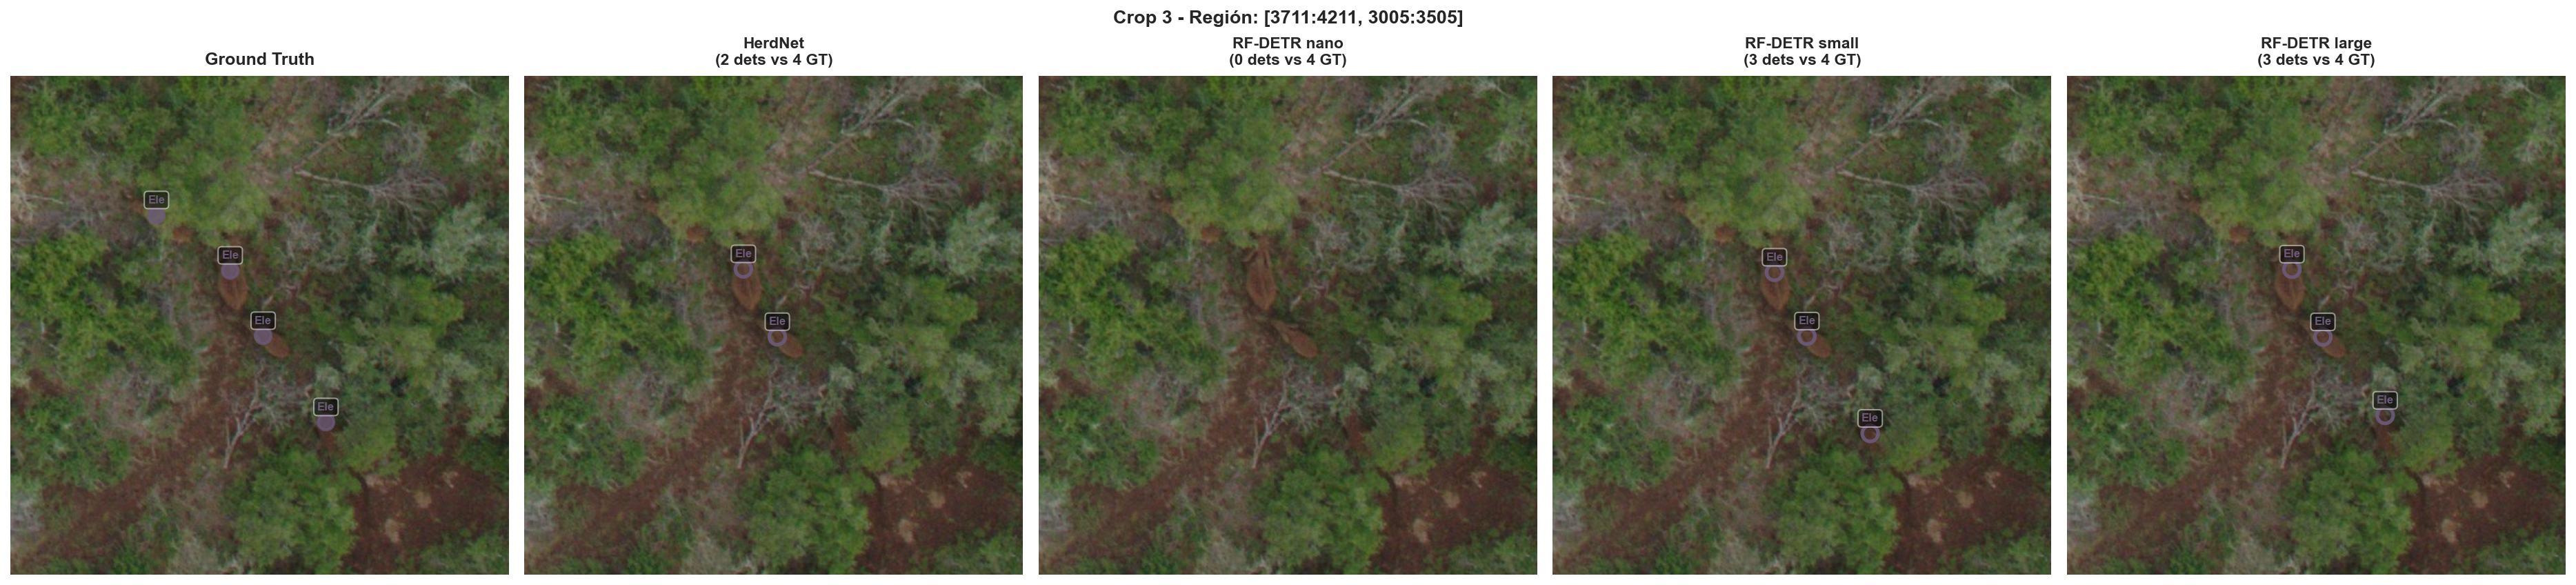
\includegraphics[width=\textwidth]{static/img/comparison_panel_elefante_crop3_stage2.png}
%     \caption{Comparación cualitativa de detecciones en escenario con oclusión severa - Elefantes. Se observan 4 elefantes parcialmente ocultos por vegetación densa.}
%     \label{fig:qualitative_elephant}
% \end{figure*}
%
% \begin{figure*}[t]
%     \centering
%     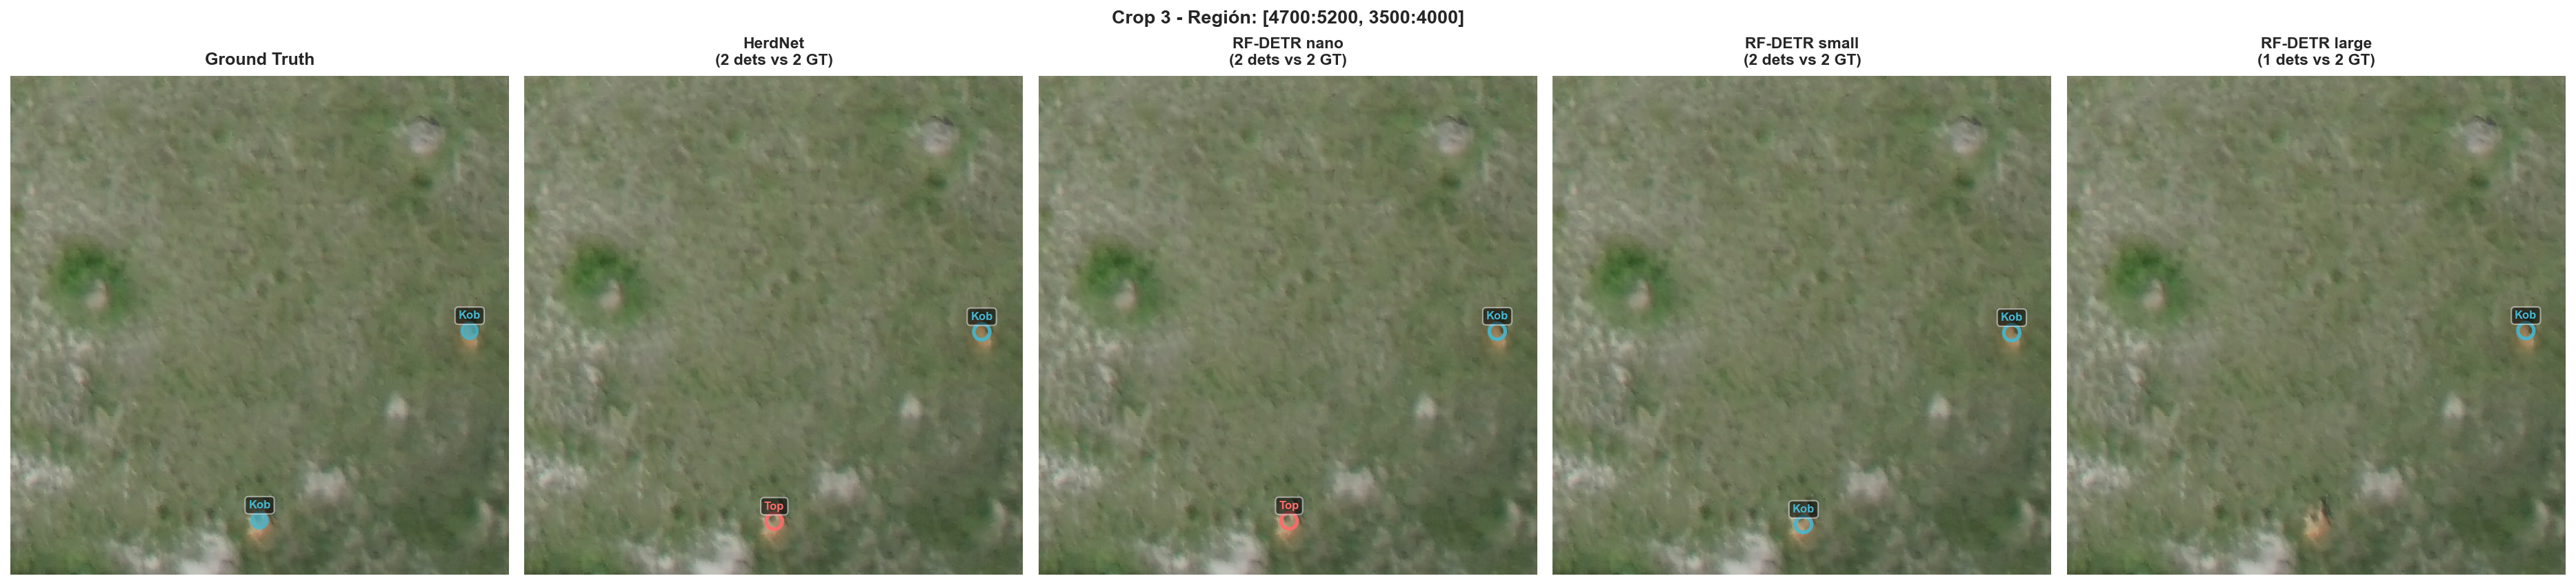
\includegraphics[width=\textwidth]{static/img/comparison_panel_facoquero_crop3_stage2.png}
%     \caption{Comparación cualitativa de detecciones en especies minoritarias - Facóquero. Se muestran 2 individuos aislados en terreno de vegetación dispersa.}
%     \label{fig:qualitative_warthog}
% \end{figure*}

\subsection{Qualitative Evaluation on Minority Species}

A qualitative evaluation focused on minority species under critical detection conditions was performed. Figures \ref{fig:qualitative_elephant} and \ref{fig:qualitative_warthog} compare model predictions against Ground Truth in two representative scenarios.

\begin{figure*}[t]
    \centering
    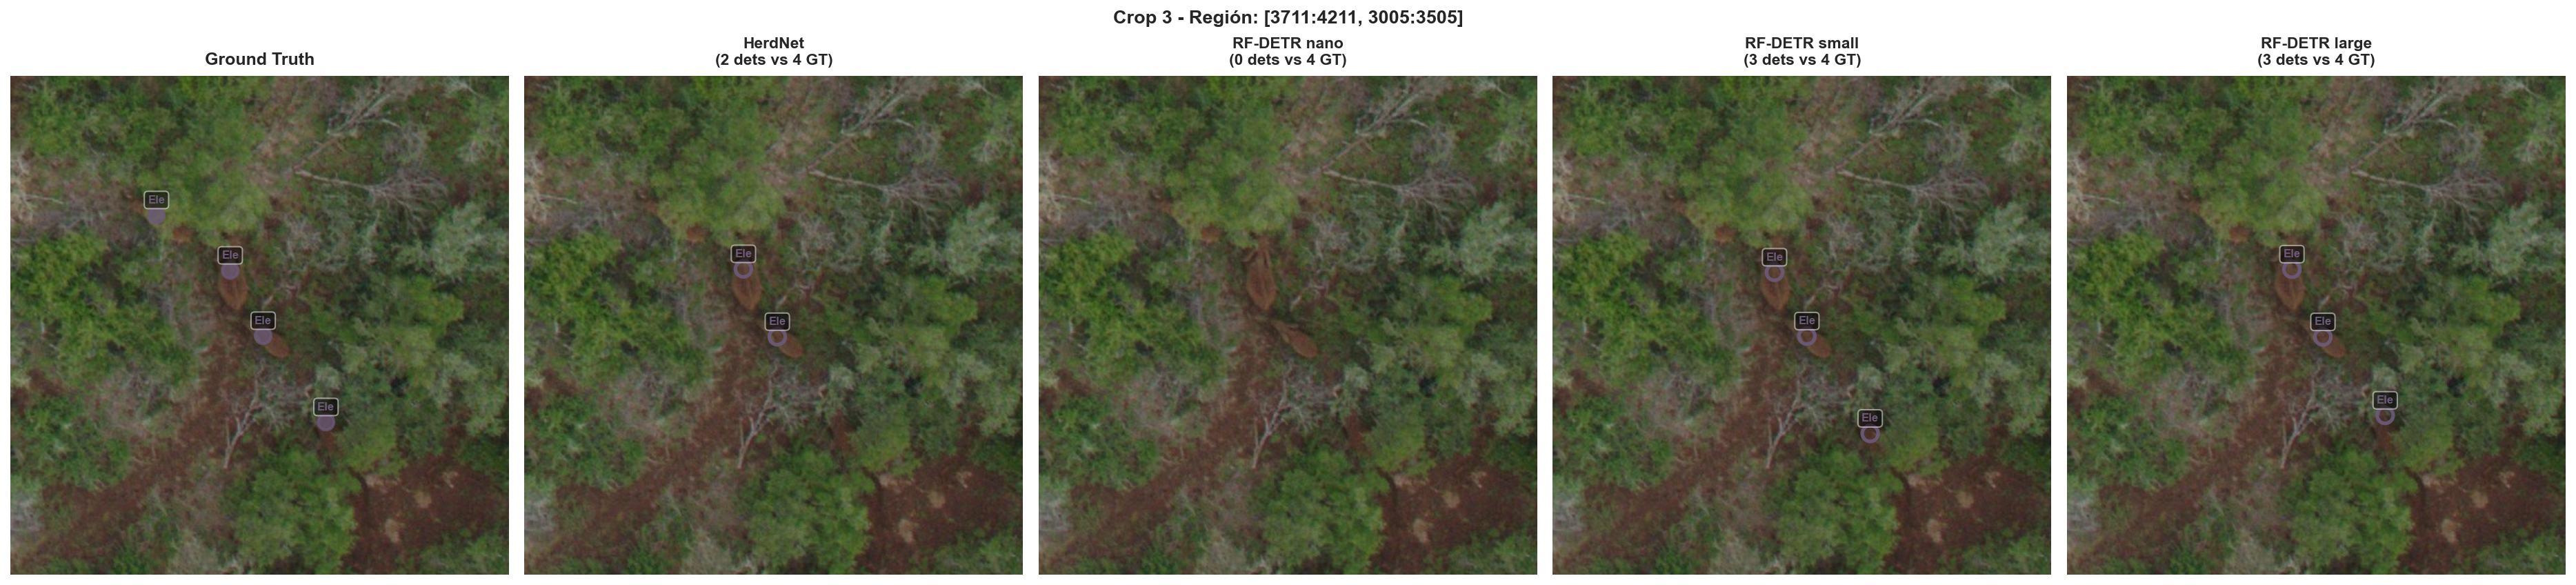
\includegraphics[width=\textwidth]{static/img/comparison_panel_elefante_crop3_stage2.png}
    \caption{Qualitative comparison of detections in a scenario with severe occlusion - Elephants. Four elephants partially hidden by dense vegetation are observed.}
    \label{fig:qualitative_elephant}
\end{figure*}

\begin{figure*}[t]
    \centering
    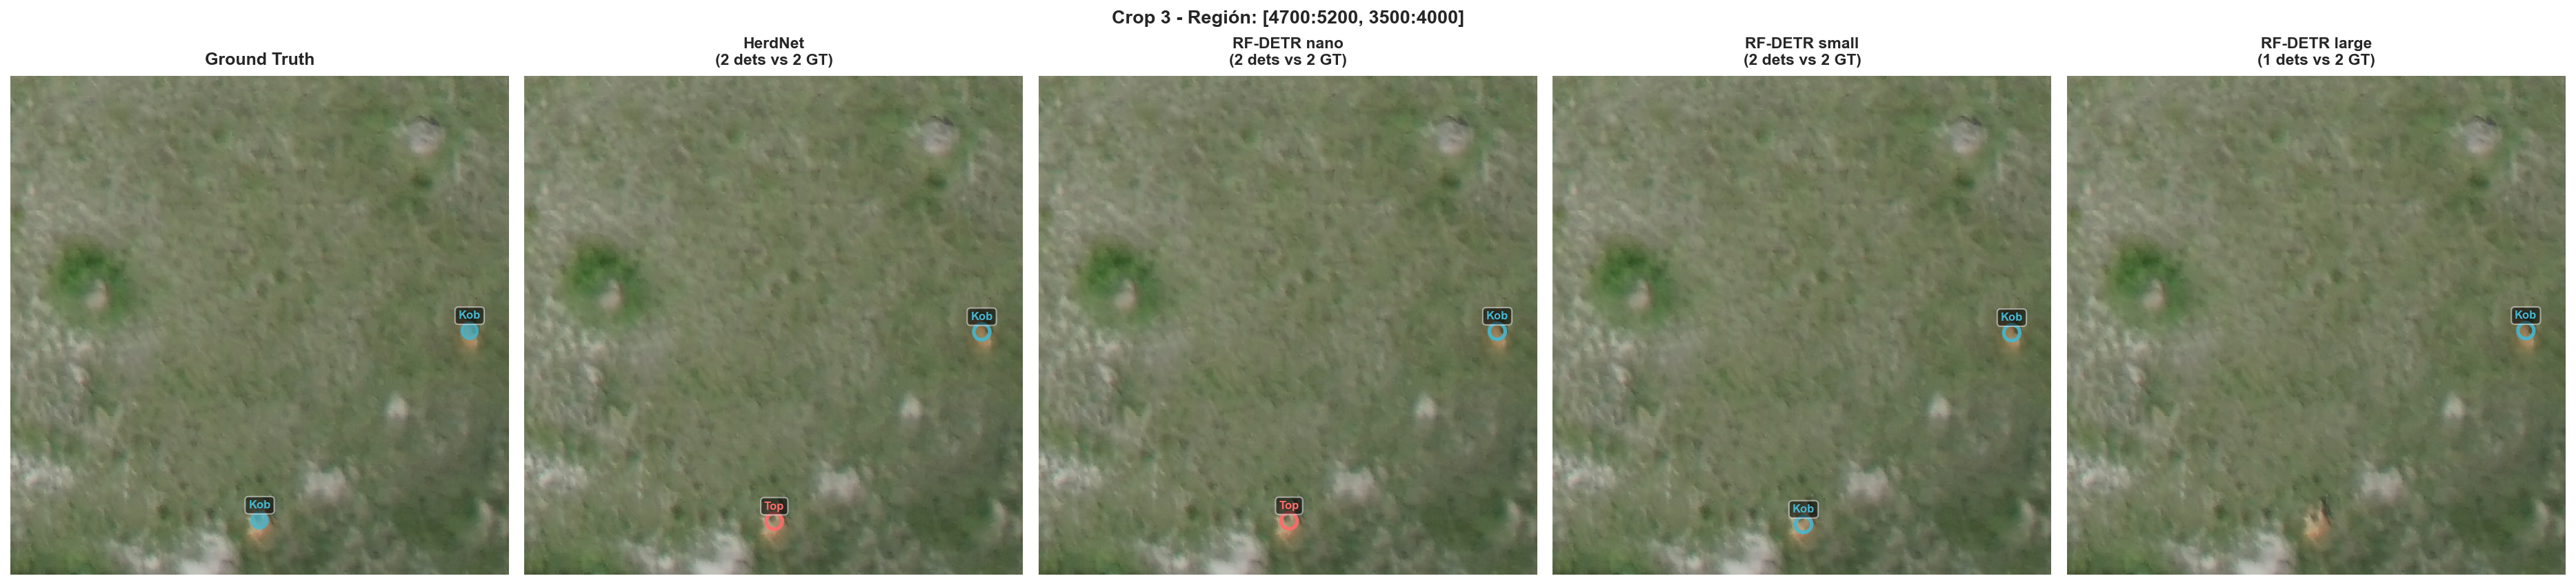
\includegraphics[width=\textwidth]{static/img/comparison_panel_facoquero_crop3_stage2.png}
    \caption{Qualitative comparison of detections on minority species - Warthog. Two isolated individuals are shown in terrain with dispersed vegetation.}
    \label{fig:qualitative_warthog}
\end{figure*}


% \subsubsection{Caso 1: Oclusión Severa en Elefantes}
%
% La Figura \ref{fig:qualitative_elephant} ilustra cuatro elefantes parcialmente ocultos por vegetación densa. Los resultados de detección son:
%
% \begin{itemize}
%     \item \textbf{HerdNet:} 2/4 detecciones (50\%). Falla en individuos con características distintivas ocultas (trompa, orejas), reflejando limitaciones del backbone ResNet-50 para capturar contexto global.
%     \item \textbf{RF-DETR small y large:} 3/4 detecciones (75\%). Mejora del +50\% sobre HerdNet, detectando exitosamente individuos con hasta 50\% de oclusión.
% \end{itemize}
%
% \textbf{Hallazgo clave:} La oclusión representa un límite fundamental para todos los modelos, incluyendo arquitecturas Transformer. Aunque RF-DETR mejora significativamente sobre HerdNet, existe un umbral de oclusión que ningún modelo supera, y \textbf{RF-DETR nano} carece de la capacidad mínima necesaria para escenarios complejos.

\subsubsection{Case 1: Severe Occlusion in Elephants}

Figure \ref{fig:qualitative_elephant} illustrates four elephants partially hidden by dense vegetation. The detection results are:

\begin{itemize}
    \item \textbf{HerdNet:} 2/4 detections (50\%). Fails on individuals with hidden distinctive features (trunk, ears), reflecting limitations of the ResNet-50 backbone to capture global context.
    \item \textbf{RF-DETR small and large:} 3/4 detections (75\%). +50\% improvement over HerdNet, successfully detecting individuals with up to 50\% occlusion.
\end{itemize}

\textbf{Key finding:} Occlusion represents a fundamental limit for all models, including Transformer architectures. Although RF-DETR significantly improves over HerdNet, there exists an occlusion threshold that no model surpasses, and \textbf{RF-DETR nano} lacks the minimum capacity necessary for complex scenarios.

% \subsubsection{Caso 2: Detección y Clasificación de Facóquero}
%
% La Figura \ref{fig:qualitative_warthog} presenta dos facóqueros en terreno abierto , revelando un patrón diferente de error: confusión en clasificación pese a detección correcta.
%
% \begin{itemize}
%     \item \textbf{HerdNet:} 2/2 detecciones pero 1/2 clasificación correcta (50\%). Detecta ambos individuos en las ubicaciones correctas pero clasifica uno erróneamente como Topi, evidenciando las limitaciones del backbone ResNet-50 para discriminar especies morfológicamente similares de tamaño medio.
%     \item \textbf{RF-DETR  small:} 2/2 detecciones y clasificación correcta (100\%). Lo que demuestra capacidad superior para discriminar Facóquero bajo condiciones de buena visibilidad, validando la efectividad del refinamiento mediante HNM y los mecanismos de atención.
% \end{itemize}
%
% \textbf{Hallazgos clave:} Este caso revela dos patrones críticos: (1) Con buena visibilidad, la detección espacial es exitosa incluso para HerdNet, pero la clasificación correcta requiere capacidades discriminativas superiores que solo los Transformers proveen. (2) Para especies minoritarias morfológicamente similares a especies mayoritarias (Facóquero vs Kob), los modelos CNN tienden a clasificar hacia la clase más frecuente, mientras que RF-DETR mantiene discriminación robusta. Esto valida la clasificación perfecta (100\%) de Facóquero reportada en la matriz de confusión para RF-DETR small.

\subsubsection{Case 2: Warthog Detection and Classification}

Figure \ref{fig:qualitative_warthog} presents two warthogs in open terrain, revealing a different error pattern: classification confusion despite correct detection.

\begin{itemize}
    \item \textbf{HerdNet:} 2/2 detections but 1/2 correct classification (50\%). Detects both individuals in the correct locations but erroneously classifies one as Topi, evidencing the limitations of the ResNet-50 backbone to discriminate morphologically similar medium-sized species.
    \item \textbf{RF-DETR small:} 2/2 detections and correct classification (100\%). This demonstrates superior capability to discriminate Warthog under good visibility conditions, validating the effectiveness of refinement through HNM and attention mechanisms.
\end{itemize}

\textbf{Key findings:} This case reveals two critical patterns: (1) With good visibility, spatial detection is successful even for HerdNet, but correct classification requires superior discriminative capabilities that only Transformers provide. (2) For minority species morphologically similar to majority species (Warthog vs Kob), CNN models tend to classify toward the most frequent class, while RF-DETR maintains robust discrimination. This validates the perfect classification (100\%) of Warthog reported in the confusion matrix for RF-DETR small.


%\section{Discusión}
\section{Discussion}

%Los resultados validan la hipótesis de que la arquitectura RF-DETR supera al baseline HerdNet gracias a su diseño libre de NMS y al uso de representaciones visuales robustas. Sin embargo, el hallazgo más relevante de este estudio no es solo la mejora en precisión, sino la identificación de la arquitectura óptima en términos de costo-beneficio.
The results validate the hypothesis that the RF-DETR architecture outperforms the HerdNet baseline thanks to its NMS-free design and the use of robust visual representations. However, the most relevant finding of this study is not only the improvement in accuracy, but the identification of the optimal architecture in terms of cost-benefit.

%\subsection{Small vs. Large: Eficiencia sobre Fuerza Bruta}
\subsection{Small vs. Large: Efficiency over Brute Force}

%Si bien se esperaba que la variante \textbf{Large} (aprox. 128M de parámetros ) dominara las métricas debido a su mayor capacidad, los resultados muestran que la variante \textbf{Small} (aprox. 32M de parámetros ) logró un rendimiento ligeramente superior en el F1-Score global (90.24\% vs 88.66\%).
While the \textbf{Large} variant (approx. 128M parameters) was expected to dominate the metrics due to its greater capacity, the results show that the \textbf{Small} variant (approx. 32M parameters) achieved slightly superior performance in the global F1-Score (90.24\% vs 88.66\%).

%Este fenómeno sugiere que el rendimiento del modelo ha alcanzado un punto de saturación respecto a la complejidad de la arquitectura para este dataset específico. Es probable que el modelo Large haya incurrido en un leve sobreajuste (\textit{overfitting}), aprendiendo detalles irrelevantes del fondo en el conjunto de entrenamiento que penalizaron su generalización en la prueba.
This phenomenon suggests that the model's performance has reached a saturation point with respect to the architecture's complexity for this specific dataset. It is likely that the Large model incurred slight overfitting (\textit{overfitting}), learning irrelevant background details in the training set that penalized its generalization on the test set.

%Por lo tanto, la principal ventaja que ofrece el modelo small radica en que logró superar al modelo más potente utilizando una fracción de los parámetros y con un tiempo de inferencia un \textbf{56\% menor} (193 ms vs 442 ms). Esto lo convierte indiscutiblemente en la mejor opción para despliegue.
Therefore, the main advantage offered by the small model lies in the fact that it managed to outperform the more powerful model using a fraction of the parameters and with an inference time \textbf{56\% lower} (193 ms vs 442 ms). This makes it indisputably the best option for deployment.

%\subsection{Análisis de Latencia: Eficiencia Estructural vs. Costo Computacional}
\subsection{Latency Analysis: Structural Efficiency vs. Computational Cost}

%El análisis de los tiempos de inferencia revela un comportamiento no lineal interesante entre las variantes \textbf{Nano} y \textbf{Small}, evidenciando un compromiso (\textit{trade-off}) entre la eficiencia del preprocesamiento y el costo computacional bruto.
The analysis of inference times reveals an interesting non-linear behavior between the \textbf{Nano} and \textbf{Small} variants, evidencing a trade-off (\textit{trade-off}) between preprocessing efficiency and raw computational cost.

%\subsubsection{Velocidad Promedio: La ventaja del modelo Small}
\subsubsection{Average Speed: The Small Model Advantage}

%En términos de latencia media, \textbf{RF-DETR Small} (193.39 ms) supera a la variante \textbf{Nano} (208.53 ms). Esto confirma la hipótesis de la \textit{Ineficiencia del Teselado}: al utilizar una resolución de entrada mayor ($512 \times 512$), el modelo Small requiere generar y ensamblar un número significativamente menor de parches para cubrir la misma área geográfica. La reducción en la sobrecarga administrativa (I/O, pre-procesamiento y fusión de resultados) compensa con creces el costo extra de inferencia por parche.
In terms of average latency, \textbf{RF-DETR Small} (193.39 ms) outperforms the \textbf{Nano} variant (208.53 ms). This confirms the hypothesis of \textit{Tiling Inefficiency}: by using a higher input resolution ($512 \times 512$), the Small model requires generating and assembling a significantly smaller number of patches to cover the same geographic area. The reduction in administrative overhead (I/O, preprocessing and result fusion) more than compensates for the extra inference cost per patch.

%\subsubsection{Latencia de Cola (P95): La estabilidad del modelo Nano}
\subsubsection{Tail Latency (P95): The Stability of the Nano Model}

%Sin embargo, en el percentil 95 (P95), la tendencia se invierte: el modelo \textbf{Nano} muestra una latencia máxima menor (317.55 ms) comparada con el \textbf{Small} (352.77 ms). Esto se debe a la física fundamental del cálculo de tensores:
However, at the 95th percentile (P95), the trend is reversed: the \textbf{Nano} model shows a lower maximum latency (317.55 ms) compared to the \textbf{Small} (352.77 ms). This is due to the fundamental physics of tensor computation:

\begin{itemize}
%    \item Un parche del modelo Small ($512^2$ px) contiene un \textbf{77\% más de píxeles} que uno del modelo Nano ($384^2$ px).
    \item A Small model patch ($512^2$ px) contains \textbf{77\% more pixels} than a Nano model patch ($384^2$ px).
%    \item En escenarios de alta carga o complejidad visual extrema, el costo cuadrático de los mecanismos de atención del Transformer sobre mapas de características más grandes penaliza al modelo Small.
    \item In high-load scenarios or extreme visual complexity, the quadratic cost of Transformer attention mechanisms over larger feature maps penalizes the Small model.
\end{itemize}

%\subsection{Small vs. Large: Eficiencia sobre Fuerza Bruta}
\subsection{Small vs. Large: Efficiency over Brute Force}

%Si bien se esperaba que la variante \textbf{Large} (aprox. 128M de parámetros ) dominara las métricas debido a su mayor capacidad, los resultados muestran que la variante \textbf{Small} (aprox. 32M de parámetros ) logró un rendimiento ligeramente superior en el F1-Score global (90.24\% vs 88.66\%).
While the \textbf{Large} variant (approx. 128M parameters) was expected to dominate the metrics due to its greater capacity, the results show that the \textbf{Small} variant (approx. 32M parameters) achieved slightly superior performance in the global F1-Score (90.24\% vs 88.66\%).

%Este fenómeno sugiere que el rendimiento del modelo ha alcanzado un punto de saturación respecto a la complejidad de la arquitectura para este dataset específico. Es probable que el modelo Large haya incurrido en un leve sobreajuste (\textit{overfitting}), aprendiendo detalles irrelevantes del fondo en el conjunto de entrenamiento que penalizaron su generalización en la prueba.
This phenomenon suggests that the model's performance has reached a saturation point with respect to the architecture's complexity for this specific dataset. It is likely that the Large model incurred slight overfitting (\textit{overfitting}), learning irrelevant background details in the training set that penalized its generalization on the test set.

%Por lo tanto, la principal ventaja que ofrece el modelo small radica en que logró superar al modelo más potente utilizando una fracción de los parámetros y con un tiempo de inferencia un \textbf{56\% menor} (193 ms vs 442 ms). Esto lo convierte indiscutiblemente en la mejor opción para despliegue.
Therefore, the main advantage offered by the small model lies in the fact that it managed to outperform the more powerful model using a fraction of the parameters and with an inference time \textbf{56\% lower} (193 ms vs 442 ms). This makes it indisputably the best option for deployment.

%\subsection{Análisis de Latencia: Eficiencia Estructural vs. Costo Computacional}
\subsection{Latency Analysis: Structural Efficiency vs. Computational Cost}

%El análisis de los tiempos de inferencia revela un comportamiento no lineal interesante entre las variantes \textbf{Nano} y \textbf{Small}, evidenciando un compromiso (\textit{trade-off}) entre la eficiencia del preprocesamiento y el costo computacional bruto.
The analysis of inference times reveals an interesting non-linear behavior between the \textbf{Nano} and \textbf{Small} variants, evidencing a trade-off (\textit{trade-off}) between preprocessing efficiency and raw computational cost.

%\subsubsection{Velocidad Promedio: La ventaja del modelo Small}
\subsubsection{Average Speed: The Small Model Advantage}

%En términos de latencia media, \textbf{RF-DETR Small} (193.39 ms) supera a la variante \textbf{Nano} (208.53 ms). Esto confirma la hipótesis de la \textit{Ineficiencia del Teselado}: al utilizar una resolución de entrada mayor ($512 \times 512$), el modelo Small requiere generar y ensamblar un número significativamente menor de parches para cubrir la misma área geográfica. La reducción en la sobrecarga administrativa (I/O, pre-procesamiento y fusión de resultados) compensa con creces el costo extra de inferencia por parche.
In terms of average latency, \textbf{RF-DETR Small} (193.39 ms) outperforms the \textbf{Nano} variant (208.53 ms). This confirms the hypothesis of \textit{Tiling Inefficiency}: by using a higher input resolution ($512 \times 512$), the Small model requires generating and assembling a significantly smaller number of patches to cover the same geographic area. The reduction in administrative overhead (I/O, preprocessing and result fusion) more than compensates for the extra inference cost per patch.

%\subsubsection{Latencia de Cola (P95): La estabilidad del modelo Nano}
\subsubsection{Tail Latency (P95): The Stability of the Nano Model}

%Sin embargo, en el percentil 95 (P95), la tendencia se invierte: el modelo \textbf{Nano} muestra una latencia máxima menor (317.55 ms) comparada con el \textbf{Small} (352.77 ms). Esto se debe a la física fundamental del cálculo de tensores:
However, at the 95th percentile (P95), the trend is reversed: the \textbf{Nano} model shows a lower maximum latency (317.55 ms) compared to the \textbf{Small} (352.77 ms). This is due to the fundamental physics of tensor computation:

\begin{itemize}
%    \item Un parche del modelo Small ($512^2$ px) contiene un \textbf{77\% más de píxeles} que uno del modelo Nano ($384^2$ px).
    \item A Small model patch ($512^2$ px) contains \textbf{77\% more pixels} than a Nano model patch ($384^2$ px).
%    \item En escenarios de alta carga o complejidad visual extrema, el costo cuadrático de los mecanismos de atención del Transformer sobre mapas de características más grandes penaliza al modelo Small.
    \item In high-load scenarios or extreme visual complexity, the quadratic cost of Transformer attention mechanisms over larger feature maps penalizes the Small model.
\end{itemize}

%Aunque las variantes \textbf{Nano} y \textbf{Small} presentan perfiles de latencia y tamaño comparables, la variante \textbf{Small} se consolida como la elección definitiva por su superioridad cualitativa. El incremento marginal en la resolución de entrada ($512 \times 512$) permite superar el umbral mínimo de representación necesario para distinguir especies críticas (como el Elefante), logrando un salto en F1-Score del 71.78\% al 90.24\% sin incurrir en los costos de la variante Large.
Although the \textbf{Nano} and \textbf{Small} variants present comparable latency and size profiles, the \textbf{Small} variant consolidates as the definitive choice due to its qualitative superiority. The marginal increase in input resolution ($512 \times 512$) allows surpassing the minimum representation threshold necessary to distinguish critical species (such as the Elephant), achieving a jump in F1-Score from 71.78\% to 90.24\% without incurring the costs of the Large variant.


%\subsection{Impacto del Hard Negative Mining (HNM)}
\subsection{Impact of Hard Negative Mining (HNM)}

%El refinamiento con HNM fue el factor determinante para la viabilidad del modelo Small. Inicialmente, este modelo presentaba una precisión baja (0.26), indicando una tendencia a alucinar animales en texturas complejas. La fase 2 corrigió drásticamente este comportamiento (precisión 0.94), demostrando que los Transformers de tamaño medio tienen la plasticidad necesaria para aprender a discriminar fondos difíciles sin necesitar la capacidad masiva (y el costo) de los modelos Large.
Refinement with HNM was the determining factor for the viability of the Small model. Initially, this model presented low precision (0.26), indicating a tendency to hallucinate animals in complex textures. Phase 2 drastically corrected this behavior (precision 0.94), demonstrating that medium-sized Transformers have the necessary plasticity to learn to discriminate difficult backgrounds without needing the massive capacity (and cost) of Large models.

%\subsection{Análisis por Especie}
\subsection{Species-Level Analysis}

%La mejora en la detección de especies minoritarias valida el uso de \textit{backbones} pre-entrenados como DINOv2. En el caso del \textit{Cobo de agua} (2.4\% del dataset), las variantes de RF-DETR mantuvieron un F1-Score robusto (mayor a 0.70), superando al baseline HerdNet. Esto indica que el modelo no requiere miles de ejemplos para aprender una representación discriminativa de una especie, un rasgo crucial para la conservación de fauna amenazada donde los datos son escasos por naturaleza.
The improvement in minority species detection validates the use of pre-trained \textit{backbones} such as DINOv2. In the case of the \textit{Waterbuck} (2.4\% of the dataset), RF-DETR variants maintained a robust F1-Score (greater than 0.70), surpassing the HerdNet baseline. This indicates that the model does not require thousands of examples to learn a discriminative representation of a species, a crucial trait for endangered wildlife conservation where data is naturally scarce.

%\subsection{Limitaciones y Oportunidades de Mejora}
\subsection{Limitations and Opportunities for Improvement}

%A pesar del éxito general del modelo \textbf{RF-DETR Small}, el análisis detallado de los resultados revela dos limitaciones técnicas importantes que definen el alcance actual de la solución y las direcciones futuras.
Despite the overall success of the \textbf{RF-DETR Small} model, detailed analysis of the results reveals two important technical limitations that define the current scope of the solution and future directions.

%\subsubsection{El Límite Inferior de la Arquitectura Nano}
\subsubsection{The Lower Bound of the Nano Architecture}

%La variante \textbf{Nano} mostró un rendimiento insuficiente (F1 global 71.78\%), colapsando dramáticamente en la clase \textit{Elefante} con un F1-Score de apenas 0.0363, en marcado contraste con el $>0.86$ logrado por las variantes Small y Large. Este fallo catastrófico establece un límite inferior claro: para distinguir patrones complejos en imágenes aéreas de alta altitud, se requiere una resolución de entrada mínima (al menos $512 \times 512$) y una profundidad de red que la versión Nano no ofrece.
The \textbf{Nano} variant showed insufficient performance (global F1 71.78\%), collapsing dramatically in the \textit{Elephant} class with an F1-Score of barely 0.0363, in stark contrast to the $>0.86$ achieved by the Small and Large variants. This catastrophic failure establishes a clear lower bound: to distinguish complex patterns in high-altitude aerial images, a minimum input resolution (at least $512 \times 512$) and network depth are required that the Nano version does not offer.

%\subsubsection{Margen de Mejora en Clases Minoritarias}
\subsubsection{Room for Improvement in Minority Classes}

%Aunque RF-DETR mejoró la detección de especies subrepresentadas respecto a HerdNet, el desempeño en clases como el \textit{Facóquero} (F1 0.4065 en Small) y el \textit{Cobo de agua} (F1 0.7097 en Small) sigue siendo inferior al de las clases mayoritarias ($>0.84$).
Although RF-DETR improved the detection of underrepresented species compared to HerdNet, performance in classes such as \textit{Warthog} (F1 0.4065 in Small) and \textit{Waterbuck} (F1 0.7097 in Small) remains lower than that of majority classes ($>0.84$).

%Es crucial notar que, a diferencia de HerdNet, el entrenamiento de RF-DETR \textbf{no implementó una ponderación agresiva de la función de pérdida} (HerdNet utilizó pesos de hasta $12$ para clases minoritarias). Esto sugiere que el rendimiento actual de RF-DETR tiene un potencial significativo para aumentar aún más la precisión en estas clases críticas mediante la incorporación de estrategias de \textit{Weighted Loss} o técnicas de sobre-muestreo (\textit{Oversampling}) específicas para las especies menos representadas.
It is crucial to note that, unlike HerdNet, RF-DETR training \textbf{did not implement aggressive loss function weighting} (HerdNet used weights of up to $12$ for minority classes). This suggests that RF-DETR's current performance has significant potential to further increase accuracy in these critical classes through the incorporation of \textit{Weighted Loss} strategies or oversampling (\textit{Oversampling}) techniques specific to less represented species.


% \section{Conclusiones y trabajo futuro}
\section{Conclusions and Future Work}

% Esta investigación ha demostrado que las arquitecturas de detección de objetos basadas en Transformers, específicamente RF-DETR, representan una solución superior para la monitorización automatizada de fauna en manadas densas, superando las limitaciones inherentes a los métodos tradicionales basados en CNN y NMS. Los hallazgos clave se resumen a continuación:
This research has demonstrated that Transformer-based object detection architectures, specifically RF-DETR, represent a superior solution for automated wildlife monitoring in dense herds, overcoming the inherent limitations of traditional CNN and NMS-based methods. The key findings are summarized below:

\begin{itemize}
    % \item \textbf{Superioridad de la Arquitectura sin NMS:} La predicción directa de conjuntos (\textit{end-to-end}) de RF-DETR resolvió eficazmente el problema de subconteo por oclusión. El modelo óptimo, \textbf{RF-DETR Small}, alcanzó un \textbf{F1-Score global de 90.24\%}, superando al baseline HerdNet (83.26\%) y reduciendo el Error Medio Absoluto (MAE) de conteo en un \textbf{39.47\%}.
    \item \textbf{Superiority of the NMS-free Architecture:} RF-DETR's direct set prediction (\textit{end-to-end}) effectively solved the occlusion-based undercounting problem. The optimal model, \textbf{RF-DETR Small}, achieved a \textbf{global F1-Score of 90.24\%}, surpassing the HerdNet baseline (83.26\%) and reducing the Mean Absolute Error (MAE) in counting by \textbf{39.47\%}.

    % \item \textbf{Eficiencia Óptima del Modelo Small:} Se identificó un punto de saturación en el rendimiento donde aumentar la complejidad del modelo no se traduce en ganancias significativas. La variante \textbf{Small} (32M parámetros) superó ligeramente a la variante \textbf{Large} (128M parámetros) en precisión global, siendo \textbf{56\% más rápida} en inferencia media (193 ms vs 442 ms), consolidándose como la opción ideal para el despliegue.
    \item \textbf{Optimal Efficiency of the Small Model:} A performance saturation point was identified where increasing model complexity does not translate into significant gains. The \textbf{Small} variant (32M parameters) slightly outperformed the \textbf{Large} variant (128M parameters) in overall precision, while being \textbf{56\% faster} in average inference (193 ms vs 442 ms), establishing itself as the ideal option for deployment.

    % \item \textbf{Validación del Hard Negative Mining:} El entrenamiento en dos fases fue crítico. La minería de negativos difíciles (HNM) transformó a RF-DETR Small de un modelo con precisión inaceptable (26.15\%) a la solución más precisa (93.85\%), demostrando la plasticidad del modelo para discriminar fondos complejos sin aumentar su tamaño.
    \item \textbf{Validation of Hard Negative Mining:} The two-phase training was critical. Hard negative mining (HNM) transformed RF-DETR Small from a model with unacceptable precision (26.15\%) to the most accurate solution (93.85\%), demonstrating the model's plasticity to discriminate complex backgrounds without increasing its size.

    % \item \textbf{Mejora en Especies Minoritarias:} El uso de \textit{backbones} visuales robustos (DINOv2) mejoró significativamente la detección de clases subrepresentadas. En el caso crítico del Cobo de agua (2.4\% del dataset), RF-DETR Small mantuvo un F1-Score robusto superior al 70\%, validando su capacidad de generalización con pocos datos.
    \item \textbf{Improvement in Minority Species:} The use of robust visual \textit{backbones} (DINOv2) significantly improved the detection of underrepresented classes. In the critical case of the Waterbuck (2.4\% of the dataset), RF-DETR Small maintained a robust F1-Score above 70\%, validating its generalization capability with limited data.

    % \item \textbf{Limitación de la Resolución Mínima:} La variante Nano demostró ser insuficiente para esta tarea, colapsando en la detección de especies clave como el Elefante, lo que establece una resolución de entrada mínima de $512 \times 512$ como requisito para capturar patrones complejos en imágenes aéreas.\newline
    \item \textbf{Minimum Resolution Limitation:} The Nano variant proved insufficient for this task, collapsing in the detection of key species such as Elephant, which establishes a minimum input resolution of $512 \times 512$ as a requirement to capture complex patterns in aerial images.\newline
\end{itemize}

% \subsubsection*{Para el trabajo futuro, se proponen dos direcciones principales}
\subsubsection*{For future work, two main directions are proposed}

\begin{enumerate}
    % \item \textbf{Mitigación Avanzada del Desbalance de Clases:}
    % Aunque RF-DETR mejoró la detección base, persiste un margen de mejora en las clases minoritarias. Se propone incorporar estrategias de ponderación de pérdida (\textit{Weighted Loss}) en la función de costo, replicando la estrategia de asignación agresiva de pesos que demostró ser efectiva en el entrenamiento de HerdNet. Alternativamente, se sugiere explorar técnicas de sobre-muestreo (\textit{Oversampling}) para equilibrar la exposición del modelo a estas especies durante el entrenamiento.
    \item \textbf{Advanced Class Imbalance Mitigation:}
    Although RF-DETR improved baseline detection, there remains room for improvement in minority classes. It is proposed to incorporate loss weighting strategies (\textit{Weighted Loss}) in the cost function, replicating the aggressive weight assignment strategy that proved effective in HerdNet training. Alternatively, it is suggested to explore oversampling techniques (\textit{Oversampling}) to balance the model's exposure to these species during training.

    % \item \textbf{Optimización de Inferencia mediante cuantización:}
    % Para facilitar el despliegue en dispositivos de borde, es necesario explorar la cuantización del modelo a INT8. Dado que las arquitecturas basadas en Transformers pueden sufrir degradación de rendimiento con una cuantización ingenua \cite{rf-detr}, se recomienda implementar esquemas de \textit{Post-Training Quantization} (PTQ) calibrados \cite{fima-q} o \textit{Quantization-Aware Training} (QAT). El objetivo es reducir la huella de memoria sin que la pérdida de precisión numérica afecte desproporcionadamente la localización en manadas densas \cite{hqod}.
    \item \textbf{Inference Optimization through Quantization:}
    To facilitate deployment on edge devices, it is necessary to explore model quantization to INT8. Given that Transformer-based architectures can suffer performance degradation with naive quantization \cite{rf-detr}, it is recommended to implement calibrated \textit{Post-Training Quantization} (PTQ) schemes \cite{fima-q} or \textit{Quantization-Aware Training} (QAT). The objective is to reduce the memory footprint without having numerical precision loss disproportionately affect localization in dense herds \cite{hqod}.

    % \item \textbf{Entrenamiento con DINOV3 como extractor de características:}
    \item \textbf{Training with DINOv3 as Feature Extractor:}

    % Si bien la implementación actual de RF-DETR utiliza DINOv2 \cite{dinov2}, la evolución reciente de la arquitectura sugiere la adopción de DINOv3 \cite{dinov3}. Se recomienda evaluar la migración hacia este nuevo backbone, dado que ha demostrado superar a su predecesor en tareas de detección, logrando un rendimiento superior con una menor cantidad de parámetros y mayor eficiencia computacional \cite{deimv2}
    While the current RF-DETR implementation uses DINOv2 \cite{dinov2}, the recent evolution of the architecture suggests the adoption of DINOv3 \cite{dinov3}. It is recommended to evaluate the migration to this new backbone, given that it has demonstrated superiority over its predecessor in detection tasks, achieving superior performance with fewer parameters and greater computational efficiency \cite{deimv2}
\end{enumerate}


\begin{thebibliography}{00}
\bibitem{xu-review} Xu, Z., Wang, T., Skidmore, A. K., \& Lamprey, R. (2024). A review of deep learning techniques for detecting animals in aerial and satellite images. International Journal of Applied Earth Observation and Geoinformation, 128, 103732. https://doi.org/10.1016/j.jag.2024.103732
\bibitem{herdnet} Delplanque, A., Foucher, S., Théau, J., Bussière, E., Vermeulen, C., \& Lejeune, P. (2023). From crowd to herd counting: How to precisely detect and count African mammals using aerial imagery and deep learning? ISPRS Journal of Photogrammetry and Remote Sensing, 197, 167–180. https://doi.org/10.1016/j.isprsjprs.2023.01.025
\bibitem{wildlife-mapper} Kumar, S., Zhang, B., Gudavalli, C., Levenson, C., Hughey, L., Stabach, J. A., Amoke, I., Ojwang, G., Mukeka, J., Mwiu, S., Ogutu, J., Frederick, H., \& Manjunath, B. S. (2024). WildlifeMapper: Aerial image analysis for multi-species detection and identification. En 2024 IEEE/CVF Conference on Computer Vision and Pattern Recognition (CVPR) (pp. 12594–12604). IEEE. https://doi.org/10.1109/CVPR52733.2024.01197
\bibitem{open-wildlife} Patel, M., Noa Turnes, J., Hsiao, J., Xu, L., \& Clausi, D. (2025). OpenWildlife: Open-vocabulary multi-species wildlife detector for geographically-diverse aerial imagery. arXiv. https://doi.org/10.48550/arXiv.2506.19204
\bibitem{rf-detr} Robinson, I., Robicheaux, P., Popov, M., Ramanan, D., \& Peri, N. (2025). RF-DETR: Neural Architecture Search for Real-Time Detection Transformers. arXiv. https://doi.org/10.48550/arXiv.2511.09554

\bibitem{dinov2} Oquab, M., Darcet, T., Moutakanni, T., Vo, H. V., Szafraniec, M., Khalidov, V., Fernandez, P., Haziza, D., Massa, F., El-Nouby, A., Assran, M., Ballas, N., Galuba, W., Howes, R., Huang, P.-Y., Li, S.-W., Misra, I., Rabbat, M., Sharma, V., ... Synnaeve, G. (2024). DINOv2: Learning robust visual features without supervision. Transactions on Machine Learning Research.

\bibitem{fima-q} Wu, Z., Wang, S., Zhang, J., Chen, J., \& Wang, Y. (2025). FIMA-Q: Post-training quantization for vision transformers by Fisher information matrix approximation. arXiv. https://doi.org/10.48550/arXiv.2506.11543

\bibitem{hqod} Huang, L., Dong, Z., Chen, S.-L., Zhang, R., Ti, S., Chen, F., \& Yin, X.-C. (2024). HQOD: Harmonious quantization for object detection. En 2024 IEEE International Conference on Multimedia and Expo (ICME) (pp. 1–6). IEEE. https://doi.org/10.1109/ICME57554.2024.10687589
\bibitem{deimv2} Huang, S., Hou, Y., Liu, L., Yu, X., \& Shen, X. (2025). Real-Time Object Detection Meets DINOv3. arXiv preprint arXiv:2509.20787. https://arxiv.org/abs/2509.20787
\bibitem{delplanque-data} Delplanque, A., Foucher, S., Lejeune, P., Linchant, J., \& Théau, J. (2021). Multispecies detection and identification of African mammals in aerial imagery using convolutional neural networks. Remote Sensing in Ecology and Conservation, 8(2), 166–179. https://doi.org/10.1002/rse2.234
\bibitem{dinov3} Siméoni, O., Vo, H. V., Seitzer, M., Baldassarre, F., Oquab, M., Jose, C., Khalidov, V., Szafraniec, M., Yi, S., Ramamonjisoa, M., Massa, F., Haziza, D., Wehrstedt, L., Wang, J., Darcet, T., Moutakanni, T., Sentana, L., Roberts, C., Vedaldi, A., Tolan, J., Brandt, J., Couprie, C., Mairal, J., Jégou, H., \& Bojanowski, P. (2025). DINOv3. arXiv preprint arXiv:2508.10104. https://arxiv.org/abs/2508.10104
\end{thebibliography}


%\clearpage
%\twocolumn[
%    \begin{center}
%        \vspace{0.5cm} % Un poco de espacio arriba
%        \textbf{\LARGE ANEXOS} % Título grande y centrado
%        \vspace{0.5cm} % Espacio antes de que empiecen las columnas
%    \end{center}
%]
\clearpage
\twocolumn[
    \begin{center}
        \vspace{0.5cm} % A bit of space above
        \textbf{\LARGE APPENDICES} % Large centered title
        \vspace{0.5cm} % Space before columns start
    \end{center}
]

%\subsection*{Anexo A. Repositorio de Código y Reproducibilidad}
\subsection*{Appendix A. Code Repository and Reproducibility}

%Para garantizar la transparencia y replicabilidad de los experimentos, el código fuente completo, los pipelines de procesamiento y los scripts de entrenamiento se encuentran disponibles públicamente en:
To ensure transparency and replicability of the experiments, the complete source code, processing pipelines, and training scripts are publicly available at:

\begin{center}
    \texttt{https://github.com/amir1226/animaldet}
\end{center}

%El entorno de desarrollo utiliza el gestor de paquetes \texttt{uv} para manejar dependencias en conflicto mediante grupos aislados (\texttt{herdnet} y \texttt{rfdetr}), asegurando que cada arquitectura se ejecute con las versiones de bibliotecas exactas utilizadas durante la investigación.
The development environment uses the \texttt{uv} package manager to handle conflicting dependencies through isolated groups (\texttt{herdnet} and \texttt{rfdetr}), ensuring that each architecture runs with the exact library versions used during the research.

%\subsection*{Anexo B. Hiperparámetros y Configuración del Entrenamiento}
\subsection*{Appendix B. Hyperparameters and Training Configuration}

%Este anexo documenta los hiperparámetros y configuraciones utilizados durante el entrenamiento de los modelos HerdNet y RF-DETR (Nano, Small, Large). Todos los entrenamientos se ejecutaron en GPU NVIDIA A100 (80GB VRAM) utilizando PyTorch 2.x y CUDA 12.x.
This appendix documents the hyperparameters and configurations used during the training of HerdNet and RF-DETR (Nano, Small, Large) models. All training runs were executed on NVIDIA A100 GPU (80GB VRAM) using PyTorch 2.x and CUDA 12.x.

%\subsubsection*{B.1 HerdNet (Baseline)}
\subsubsection*{B.1 HerdNet (Baseline)}

%\paragraph{Fase 1 - Entrenamiento Inicial}
\paragraph{Phase 1 - Initial Training}
\begin{itemize}
%    \item \textbf{Épocas:} 100
    \item \textbf{Epochs:} 100
%    \item \textbf{Learning Rate Inicial:} $1 \times 10^{-4}$
    \item \textbf{Initial Learning Rate:} $1 \times 10^{-4}$
%    \item \textbf{Optimizador:} Adam
    \item \textbf{Optimizer:} Adam
%    \item \textbf{Weight Decay:} $5 \times 10^{-4}$
    \item \textbf{Weight Decay:} $5 \times 10^{-4}$
%    \item \textbf{Batch Size:} 4
    \item \textbf{Batch Size:} 4
%    \item \textbf{Learning Rate Schedule:} ReduceLROnPlateau
    \item \textbf{Learning Rate Schedule:} ReduceLROnPlateau
    \begin{itemize}
%        \item Mode: max (monitorea F1-Score)
        \item Mode: max (monitors F1-Score)
%        \item Patience: 10 épocas
        \item Patience: 10 epochs
%        \item Threshold: $1 \times 10^{-4}$
        \item Threshold: $1 \times 10^{-4}$
%        \item Cooldown: 10 épocas
        \item Cooldown: 10 epochs
%        \item Min LR: $1 \times 10^{-6}$
        \item Min LR: $1 \times 10^{-6}$
    \end{itemize}
%    \item \textbf{Tamaño de parche:} $512 \times 512$ píxeles
    \item \textbf{Patch Size:} $512 \times 512$ pixels
%    \item \textbf{Down Ratio:} 2 (para localización)
    \item \textbf{Down Ratio:} 2 (for localization)
%    \item \textbf{Warmup Iterations:} 100
    \item \textbf{Warmup Iterations:} 100
\end{itemize}

%\paragraph{Funciones de Pérdida (Fase 1)}
\paragraph{Loss Functions (Phase 1)}
\begin{itemize}
%    \item \textbf{Localización:} Focal Loss (reduction='mean', normalize=False)
    \item \textbf{Localization:} Focal Loss (reduction='mean', normalize=False)
%    \item \textbf{Clasificación:} Weighted Cross-Entropy Loss
    \item \textbf{Classification:} Weighted Cross-Entropy Loss
%    \item \textbf{Pesos por clase:} $w = [0.1, 1.0, 2.0, 1.0, 6.0, 12.0, 1.0]$
    \item \textbf{Class Weights:} $w = [0.1, 1.0, 2.0, 1.0, 6.0, 12.0, 1.0]$
\end{itemize}

%\paragraph{Fase 2 - Hard Negative Mining}
\paragraph{Phase 2 - Hard Negative Mining}
\begin{itemize}
%    \item \textbf{Épocas:} 50
    \item \textbf{Epochs:} 50
%    \item \textbf{Learning Rate Inicial:} $1 \times 10^{-6}$ (reducido 100×)
    \item \textbf{Initial Learning Rate:} $1 \times 10^{-6}$ (reduced 100×)
%    \item \textbf{Optimizador:} Adam
    \item \textbf{Optimizer:} Adam
%    \item \textbf{Weight Decay:} $5 \times 10^{-4}$
    \item \textbf{Weight Decay:} $5 \times 10^{-4}$
%    \item \textbf{Batch Size:} 4
    \item \textbf{Batch Size:} 4
%    \item \textbf{Warmup Iterations:} 1
    \item \textbf{Warmup Iterations:} 1
%    \item \textbf{Validation Frequency:} Cada 10 épocas
    \item \textbf{Validation Frequency:} Every 10 epochs
%    \item \textbf{Pesos por clase:} Idénticos a Fase 1
    \item \textbf{Class Weights:} Identical to Phase 1
%    \item \textbf{Checkpoint Inicial:} Mejor modelo de Fase 1 (selección por F1-Score máximo)
    \item \textbf{Initial Checkpoint:} Best Phase 1 model (selected by maximum F1-Score)
\end{itemize}

%\subsubsection*{B.2 RF-DETR (Todas las variantes)}
\subsubsection*{B.2 RF-DETR (All variants)}

%La Tabla \ref{tab:rfdetr_hyperparams} resume los hiperparámetros para las tres variantes de RF-DETR. Se destacan las diferencias en la resolución de entrada y la cantidad de parámetros.
Table \ref{tab:rfdetr_hyperparams} summarizes the hyperparameters for the three RF-DETR variants. The differences in input resolution and number of parameters are highlighted.

\begin{table}[htbp]
\centering
%\caption{Hiperparámetros de entrenamiento para RF-DETR (Nano, Small, Large).}
\caption{Training hyperparameters for RF-DETR (Nano, Small, Large).}
\label{tab:rfdetr_hyperparams}
\resizebox{\columnwidth}{!}{%
\begin{tabular}{lccc}
\hline
%\textbf{Parámetro} & \textbf{Nano} & \textbf{Small} & \textbf{Large} \\ \hline
\textbf{Parameter} & \textbf{Nano} & \textbf{Small} & \textbf{Large} \\ \hline
%\multicolumn{4}{l}{\textit{Arquitectura}} \\
\multicolumn{4}{l}{\textit{Architecture}} \\
%Tamaño de Entrada & $384 \times 384$ & $512 \times 512$ & $560 \times 560$ \\
Input Size & $384 \times 384$ & $512 \times 512$ & $560 \times 560$ \\
Backbone Base & DINOv2 & DINOv2 & DINOv2 \\
%Parámetros (aprox.) & \textbf{30.5 M} & \textbf{32.1 M} & \textbf{128 M} \\ \hline
Parameters (approx.) & \textbf{30.5 M} & \textbf{32.1 M} & \textbf{128 M} \\ \hline
%\multicolumn{4}{l}{\textit{Fase 1 - Entrenamiento Inicial}} \\
\multicolumn{4}{l}{\textit{Phase 1 - Initial Training}} \\
%Épocas & 50 & 50 & 50 \\
Epochs & 50 & 50 & 50 \\
Batch Size & 16 & 16 & 16 \\
Grad Accum Steps & 4 & 4 & 4 \\
%\textbf{Batch Efectivo} & \textbf{64} & \textbf{64} & \textbf{64} \\
\textbf{Effective Batch} & \textbf{64} & \textbf{64} & \textbf{64} \\
Learning Rate & Default* & Default* & Default* \\
%Optimizador & AdamW & AdamW & AdamW \\ \hline
Optimizer & AdamW & AdamW & AdamW \\ \hline
%\multicolumn{4}{l}{\textit{Fase 2 - Hard Negative Mining}} \\
\multicolumn{4}{l}{\textit{Phase 2 - Hard Negative Mining}} \\
%Épocas & 50 & 50 & 50 \\
Epochs & 50 & 50 & 50 \\
Batch Size & 2 & 2 & 2 \\
Grad Accum Steps & 8 & 8 & 8 \\
%\textbf{Batch Efectivo} & \textbf{16} & \textbf{16} & \textbf{16} \\
\textbf{Effective Batch} & \textbf{16} & \textbf{16} & \textbf{16} \\
Learning Rate (Decoder) & $1 \times 10^{-5}$ & $1 \times 10^{-5}$ & $1 \times 10^{-5}$ \\
Learning Rate (Encoder) & $1 \times 10^{-5}$ & $1 \times 10^{-5}$ & $1 \times 10^{-5}$ \\
Weight Decay & $1 \times 10^{-4}$ & $1 \times 10^{-4}$ & $1 \times 10^{-4}$ \\
EMA Decay & 0.993 & 0.993 & 0.993 \\
Multi-Scale Training & \checkmark & \checkmark & \checkmark \\
\hline
\end{tabular}%
}
\end{table}

%\textit{*Default: Learning rate con decaimiento por capas (layer-wise decay) según configuración estándar del framework RF-DETR $1 \times 10^{-4}$.}
\textit{*Default: Learning rate with layer-wise decay according to standard RF-DETR framework configuration $1 \times 10^{-4}$.}

\FloatBarrier

%\subsection*{Anexo C. Métricas Detalladas por Especie}
\subsection*{Appendix C. Detailed Metrics by Species}

%Este anexo presenta una desagregación completa de las métricas de rendimiento por especie para los cuatro modelos evaluados (HerdNet, RF-DETR Nano, RF-DETR Small, RF-DETR Large) en la Fase 2 del entrenamiento (con HNM). Las tablas permiten analizar el desempeño específico de cada arquitectura en el manejo de especies minoritarias y mayoritarias.
This appendix presents a complete breakdown of performance metrics by species for the four evaluated models (HerdNet, RF-DETR Nano, RF-DETR Small, RF-DETR Large) in Phase 2 of training (with HNM). The tables allow for analyzing the specific performance of each architecture in handling minority and majority species.

%\subsubsection*{C.1 Topi}
\subsubsection*{C.1 Topi}

%El Topi representa una de las especies mayoritarias del dataset (2.722 individuos, 26.6\% del total). La Tabla \ref{tab:metrics_topi} muestra que todos los modelos alcanzan un rendimiento elevado en esta especie, con F1-Scores superiores al 83\%.
The Topi represents one of the majority species in the dataset (2,722 individuals, 26.6\% of the total). Table \ref{tab:metrics_topi} shows that all models achieve high performance on this species, with F1-Scores exceeding 83\%.

\begin{table}[ht]
\centering
%\caption{Métricas de rendimiento para la especie Topi (Fase 2).}
\caption{Performance metrics for the Topi species (Phase 2).}
\label{tab:metrics_topi}
\resizebox{\columnwidth}{!}{%
\begin{tabular}{lcccc}
\hline
%\textbf{Métrica} & \textbf{HerdNet} & \textbf{RF-DETR Nano} & \textbf{RF-DETR Small} & \textbf{RF-DETR Large} \\ \hline
\textbf{Metric} & \textbf{HerdNet} & \textbf{RF-DETR Nano} & \textbf{RF-DETR Small} & \textbf{RF-DETR Large} \\ \hline
F1-Score & 0.8559 & 0.8381 & \textbf{0.8960} & 0.8550 \\
Precision & 0.8371 & 0.7615 & \textbf{0.8800} & 0.7909 \\
Recall & 0.8756 & 0.9319 & 0.9126 & \textbf{0.9304} \\
MAE & 1.7042 & 2.1059 & \textbf{1.5735} & 1.9615 \\
RMSE & 2.8009 & 3.4007 & \textbf{2.9180} & 3.3722 \\ \hline
\end{tabular}%
}
\end{table}

%\subsubsection*{C.2 Búfalo}
\subsubsection*{C.2 Buffalo}

%El Búfalo es otra especie mayoritaria del dataset (1.509 individuos, 14.7\% del total). La Tabla \ref{tab:metrics_buffalo} revela un patrón de rendimiento similar al Topi, con mejoras consistentes de RF-DETR Small.
The Buffalo is another majority species in the dataset (1,509 individuals, 14.7\% of the total). Table \ref{tab:metrics_buffalo} reveals a performance pattern similar to Topi, with consistent improvements from RF-DETR Small.

\begin{table}[ht]
\centering
%\caption{Métricas de rendimiento para la especie Búfalo (Fase 2).}
\caption{Performance metrics for the Buffalo species (Phase 2).}
\label{tab:metrics_buffalo}
\resizebox{\columnwidth}{!}{%
\begin{tabular}{lcccc}
\hline
%\textbf{Métrica} & \textbf{HerdNet} & \textbf{RF-DETR Nano} & \textbf{RF-DETR Small} & \textbf{RF-DETR Large} \\ \hline
\textbf{Metric} & \textbf{HerdNet} & \textbf{RF-DETR Nano} & \textbf{RF-DETR Small} & \textbf{RF-DETR Large} \\ \hline
F1-Score & 0.8115 & 0.8024 & \textbf{0.8435} & 0.8313 \\
Precision & 0.9170 & 0.8471 & \textbf{0.9531} & 0.8944 \\
Recall & 0.7278 & 0.7622 & 0.7564 & \textbf{0.7765} \\
MAE & 3.5000 & 3.1786 & 3.3333 & \textbf{3.0400} \\
RMSE & 5.9702 & 6.2593 & 6.4936 & \textbf{5.9464} \\ \hline
\end{tabular}%
}
\end{table}

%\subsubsection*{C.3 Kob}
\subsubsection*{C.3 Kob}

%El Kob es una especie mayoritaria del dataset (2.370 individuos, 23.1\% del total). La Tabla \ref{tab:metrics_kob} muestra un rendimiento excepcional de RF-DETR Small.
The Kob is a majority species in the dataset (2,370 individuals, 23.1\% of the total). Table \ref{tab:metrics_kob} shows exceptional performance from RF-DETR Small.

\begin{table}[ht]
\centering
%\caption{Métricas de rendimiento para la especie Kob (Fase 2).}
\caption{Performance metrics for the Kob species (Phase 2).}
\label{tab:metrics_kob}
\resizebox{\columnwidth}{!}{%
\begin{tabular}{lcccc}
\hline
%\textbf{Métrica} & \textbf{HerdNet} & \textbf{RF-DETR Nano} & \textbf{RF-DETR Small} & \textbf{RF-DETR Large} \\ \hline
\textbf{Metric} & \textbf{HerdNet} & \textbf{RF-DETR Nano} & \textbf{RF-DETR Small} & \textbf{RF-DETR Large} \\ \hline
F1-Score & 0.8751 & 0.8156 & \textbf{0.9051} & 0.8019 \\
Precision & 0.8484 & 0.7812 & \textbf{0.9432} & 0.9029 \\
Recall & \textbf{0.9036} & 0.8532 & 0.8700 & 0.7212 \\
MAE & 1.0283 & 1.2952 & \textbf{0.6915} & 1.5506 \\
RMSE & 1.9882 & 2.1647 & \textbf{1.8072} & 3.2568 \\ \hline
\end{tabular}%
}
\end{table}


%\subsubsection*{C.4 Facóquero}
\subsubsection*{C.4 Warthog}

%El Facóquero es una especie minoritaria del dataset (433 individuos, 4.2\% del total). La Tabla \ref{tab:metrics_warthog} revela uno de los desafíos más significativos del estudio: todos los modelos presentan un rendimiento limitado en esta clase.
The Warthog is a minority species in the dataset (433 individuals, 4.2\% of the total). Table \ref{tab:metrics_warthog} reveals one of the most significant challenges of the study: all models exhibit limited performance on this class.

\begin{table}[ht]
\centering
%\caption{Métricas de rendimiento para la especie Facóquero (Fase 2).}
\caption{Performance metrics for the Warthog species (Phase 2).}
\label{tab:metrics_warthog}
\resizebox{\columnwidth}{!}{%
\begin{tabular}{lcccc}
\hline
%\textbf{Métrica} & \textbf{HerdNet} & \textbf{RF-DETR Nano} & \textbf{RF-DETR Small} & \textbf{RF-DETR Large} \\ \hline
\textbf{Metric} & \textbf{HerdNet} & \textbf{RF-DETR Nano} & \textbf{RF-DETR Small} & \textbf{RF-DETR Large} \\ \hline
F1-Score & 0.4151 & 0.3788 & 0.4065 & \textbf{0.4493} \\
Precision & 0.3882 & 0.4310 & 0.5102 & \textbf{0.4844} \\
Recall & \textbf{0.4459} & \textbf{0.3378} & \textbf{0.3378} & \textbf{0.4189} \\
MAE & 2.2432 & 2.4667 & 2.4815 & \textbf{2.4000} \\
RMSE & \textbf{3.1322} & 3.5496 & 3.5013 & 3.4351 \\ \hline
\end{tabular}%
}
\end{table}

%\subsubsection*{C.5 Cobo de agua}
\subsubsection*{C.5 Waterbuck}

%El Cobo de agua es la especie más minoritaria del dataset (241 individuos, 2.4\% del total). La Tabla \ref{tab:metrics_waterbuck} muestra el impacto más pronunciado de las arquitecturas basadas en Transformers.
The Waterbuck is the most minority species in the dataset (241 individuals, 2.4\% of the total). Table \ref{tab:metrics_waterbuck} shows the most pronounced impact of Transformer-based architectures.

\begin{table}[ht]
\centering
%\caption{Métricas de rendimiento para la especie Cobo de agua (Fase 2).}
\caption{Performance metrics for the Waterbuck species (Phase 2).}
\label{tab:metrics_waterbuck}
\resizebox{\columnwidth}{!}{%
\begin{tabular}{lcccc}
\hline
%\textbf{Métrica} & \textbf{HerdNet} & \textbf{RF-DETR Nano} & \textbf{RF-DETR Small} & \textbf{RF-DETR Large} \\ \hline
\textbf{Metric} & \textbf{HerdNet} & \textbf{RF-DETR Nano} & \textbf{RF-DETR Small} & \textbf{RF-DETR Large} \\ \hline
F1-Score & 0.6849 & 0.6237 & 0.7097 & \textbf{0.8158} \\
Precision & 0.6757 & 0.5088 & 0.8462 & \textbf{0.7750} \\
Recall & 0.6944 & \textbf{0.8056} & 0.6111 & \textbf{0.8611} \\
MAE & 1.2500 & 1.4375 & 2.5714 & \textbf{1.2000} \\
RMSE & 1.5000 & 2.2500 & 3.0237 & \textbf{1.4142} \\ \hline
\end{tabular}%
}
\end{table}

%\subsubsection*{C.6 Elefante}
\subsubsection*{C.6 Elephant}

%El Elefante es la especie más numerosa del dataset (2.964 individuos, 28.9\% del total). La Tabla \ref{tab:metrics_elephant} revela el fallo de RF-DETR Nano en esta clase.
The Elephant is the most numerous species in the dataset (2,964 individuals, 28.9\% of the total). Table \ref{tab:metrics_elephant} reveals the failure of RF-DETR Nano on this class.

\begin{table}[ht]
\centering
%\caption{Métricas de rendimiento para la especie Elefante (Fase 2).}
\caption{Performance metrics for the Elephant species (Phase 2).}
\label{tab:metrics_elephant}
\resizebox{\columnwidth}{!}{%
\begin{tabular}{lcccc}
\hline
%\textbf{Métrica} & \textbf{HerdNet} & \textbf{RF-DETR Nano} & \textbf{RF-DETR Small} & \textbf{RF-DETR Large} \\ \hline
\textbf{Metric} & \textbf{HerdNet} & \textbf{RF-DETR Nano} & \textbf{RF-DETR Small} & \textbf{RF-DETR Large} \\ \hline
F1-Score & 0.6956 & 0.0363 & 0.8649 & \textbf{0.8641} \\
Precision & 0.6707 & 0.4483 & 0.8995 & \textbf{0.8549} \\
Recall & 0.7224 & 0.0189 & 0.8328 & \textbf{0.8735} \\
MAE & 2.5728 & 6.5900 & \textbf{1.0700} & 1.2300 \\
RMSE & 4.4142 & 10.3068 & \textbf{1.5969} & 3.9154 \\ \hline
\end{tabular}%
}
\end{table}

\FloatBarrier

%\subsection*{Anexo D. Ejemplos Cualitativos Adicionales}
\subsection*{Appendix D. Additional Qualitative Examples}

%A continuación, la Figura \ref{fig:anexo_c_1} ilustra los resultados de detección para el Cobo de agua. Esta comparación cualitativa sobre 4 individuos permite visualizar el desempeño de los modelos en una de las especies con menor representación (minoritaria) en el conjunto de entrenamiento.
The following Figure \ref{fig:anexo_c_1} illustrates the detection results for the Waterbuck. This qualitative comparison on 4 individuals allows visualizing the performance of the models on one of the species with the least representation (minority) in the training set.
\begin{figure}[ht]
    \centering
    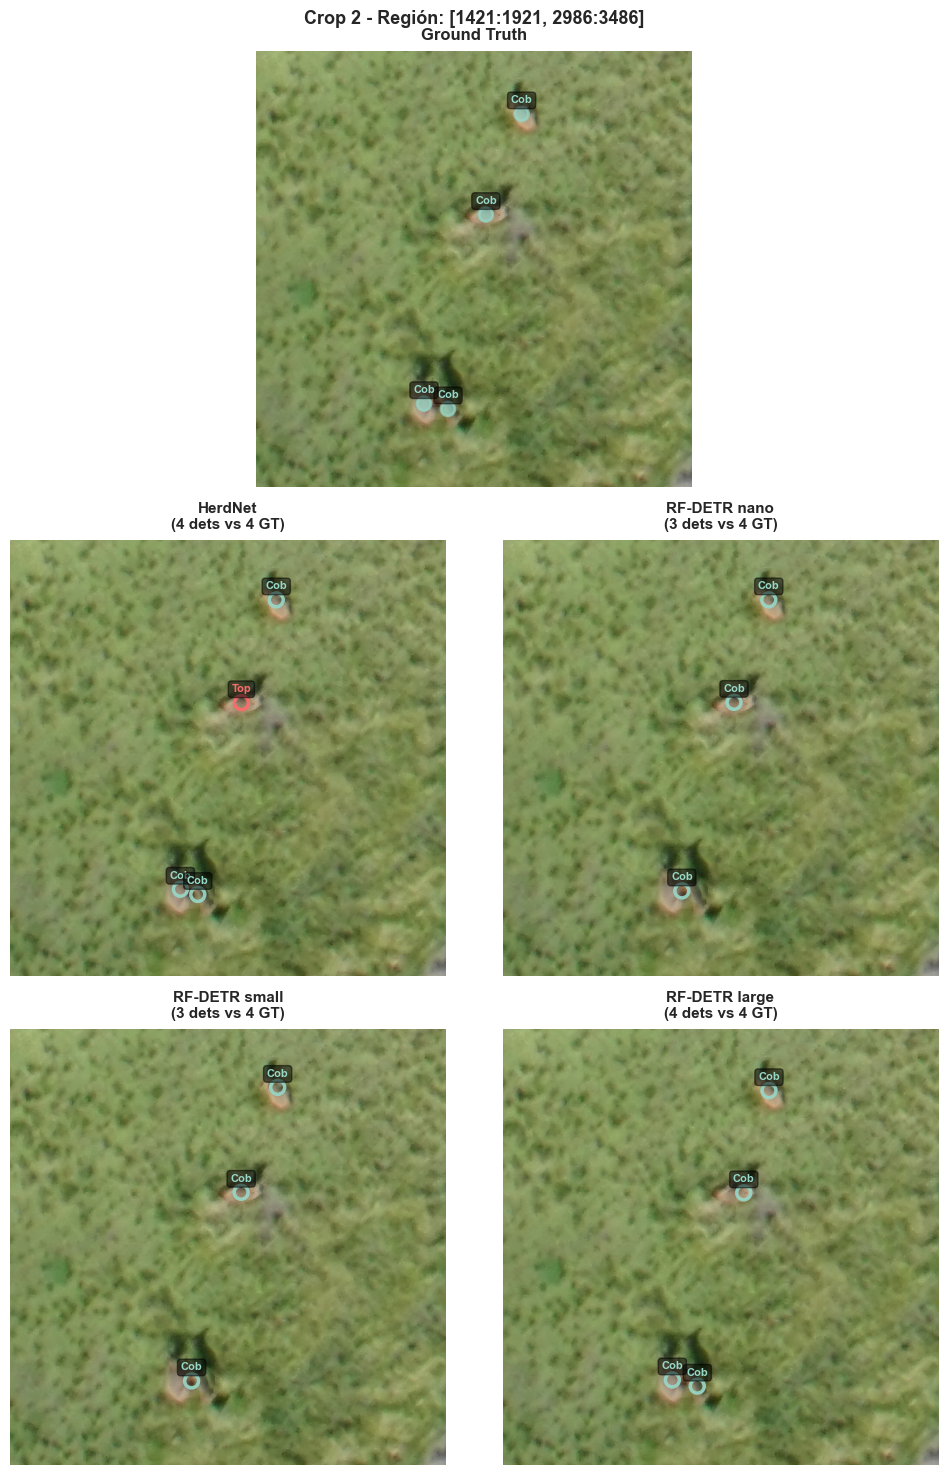
\includegraphics[width=0.9\columnwidth, height=1.78\columnwidth]{static/img/anexo_c_comp_1.png}
%    \caption{Comparación cualitativa del cobo de agua. Se observan 4 cobos de agua.}
    \caption{Qualitative comparison of the waterbuck. 4 waterbucks are observed.}
    \label{fig:anexo_c_1}
\end{figure}

\FloatBarrier
%La Figura \ref{fig:anexo_c_2} presenta un escenario con 2 individuos de la especie Topi. Esta comparación sirve para evaluar la precisión de clasificación y localización en una de las especies de antílopes más frecuentes y de tamaño medio del conjunto de datos.
Figure \ref{fig:anexo_c_2} presents a scenario with 2 individuals of the Topi species. This comparison serves to evaluate the classification and localization accuracy on one of the most frequent medium-sized antelope species in the dataset.

\begin{figure}[ht]
    \centering
    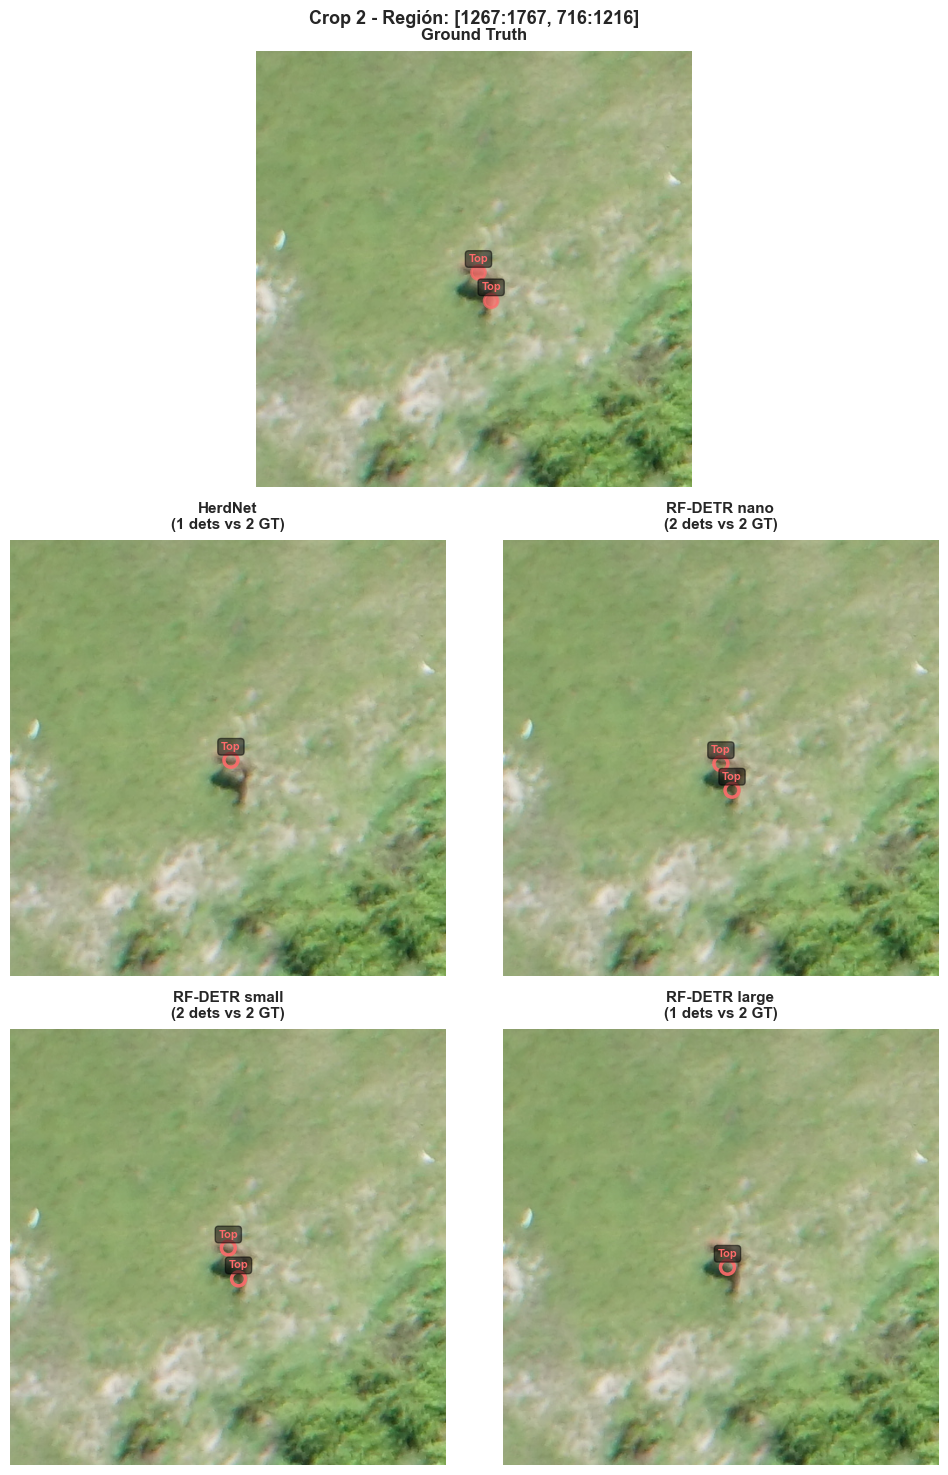
\includegraphics[width=0.9\columnwidth, height=2.25\columnwidth]{static/img/anexo_c_comp_2.png}
%    \caption{Comparación cualitativa del topi. Se observan 2 topis.}
    \caption{Qualitative comparison of the topi. 2 topis are observed.}
    \label{fig:anexo_c_2}
\end{figure}
\FloatBarrier
%En la siguiente Figura \ref{fig:anexo_c_3} se visualizan los resultados para el Facóquero. Este ejemplo con 3 individuos es crítico para analizar la capacidad de los diferentes modelos para detectar objetivos de tamaño muy pequeño, un desafío donde suelen ocurrir omisiones (falsos negativos).
In the following Figure \ref{fig:anexo_c_3} the results for the Warthog are visualized. This example with 3 individuals is critical for analyzing the capability of the different models to detect very small-sized targets, a challenge where omissions (false negatives) often occur.

\begin{figure}[ht]
    \centering
    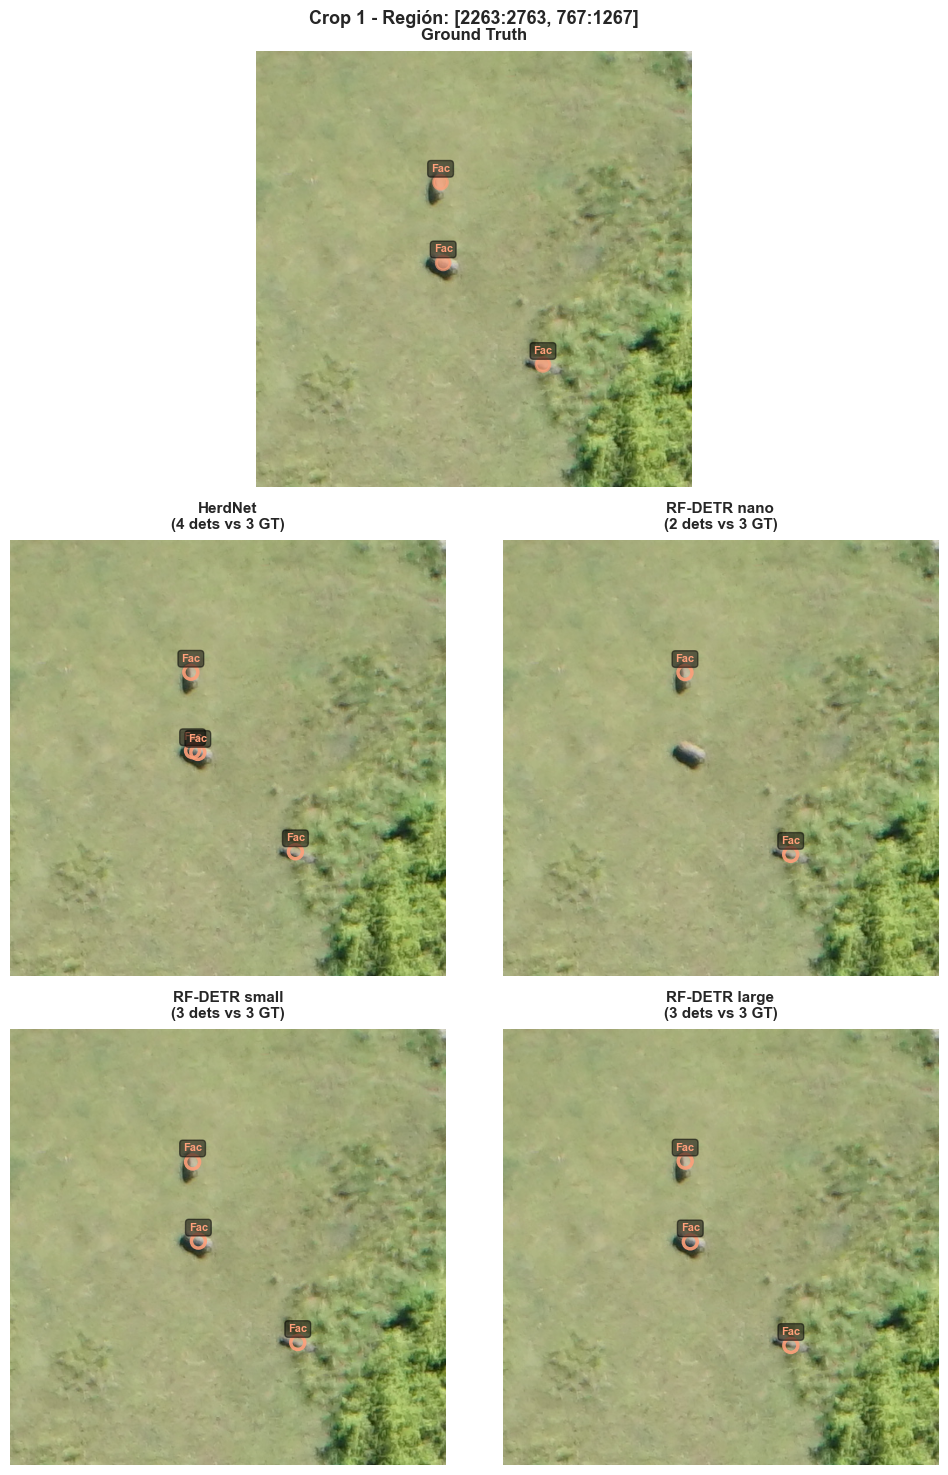
\includegraphics[width=0.9\columnwidth, height=2.25\columnwidth]{static/img/anexo_c_comp_3.png}
%    \caption{Comparación cualitativa del Facóquero. Se observan 2 facóqueros.}
    \caption{Qualitative comparison of the Warthog. 2 warthogs are observed.}
    \label{fig:anexo_c_3}
\end{figure}
\FloatBarrier
%Por último, la Figura \ref{fig:anexo_c_4} presenta una comparación cualitativa sobre un grupo de 6 Búfalos. Este escenario permite observar el comportamiento de los detectores ante una especie de gran tamaño, coloración oscura y morfología distintiva.
Finally, Figure \ref{fig:anexo_c_4} presents a qualitative comparison on a group of 6 Buffalos. This scenario allows observing the behavior of the detectors when faced with a large-sized species with dark coloration and distinctive morphology.

\begin{figure}[ht]
    \centering
    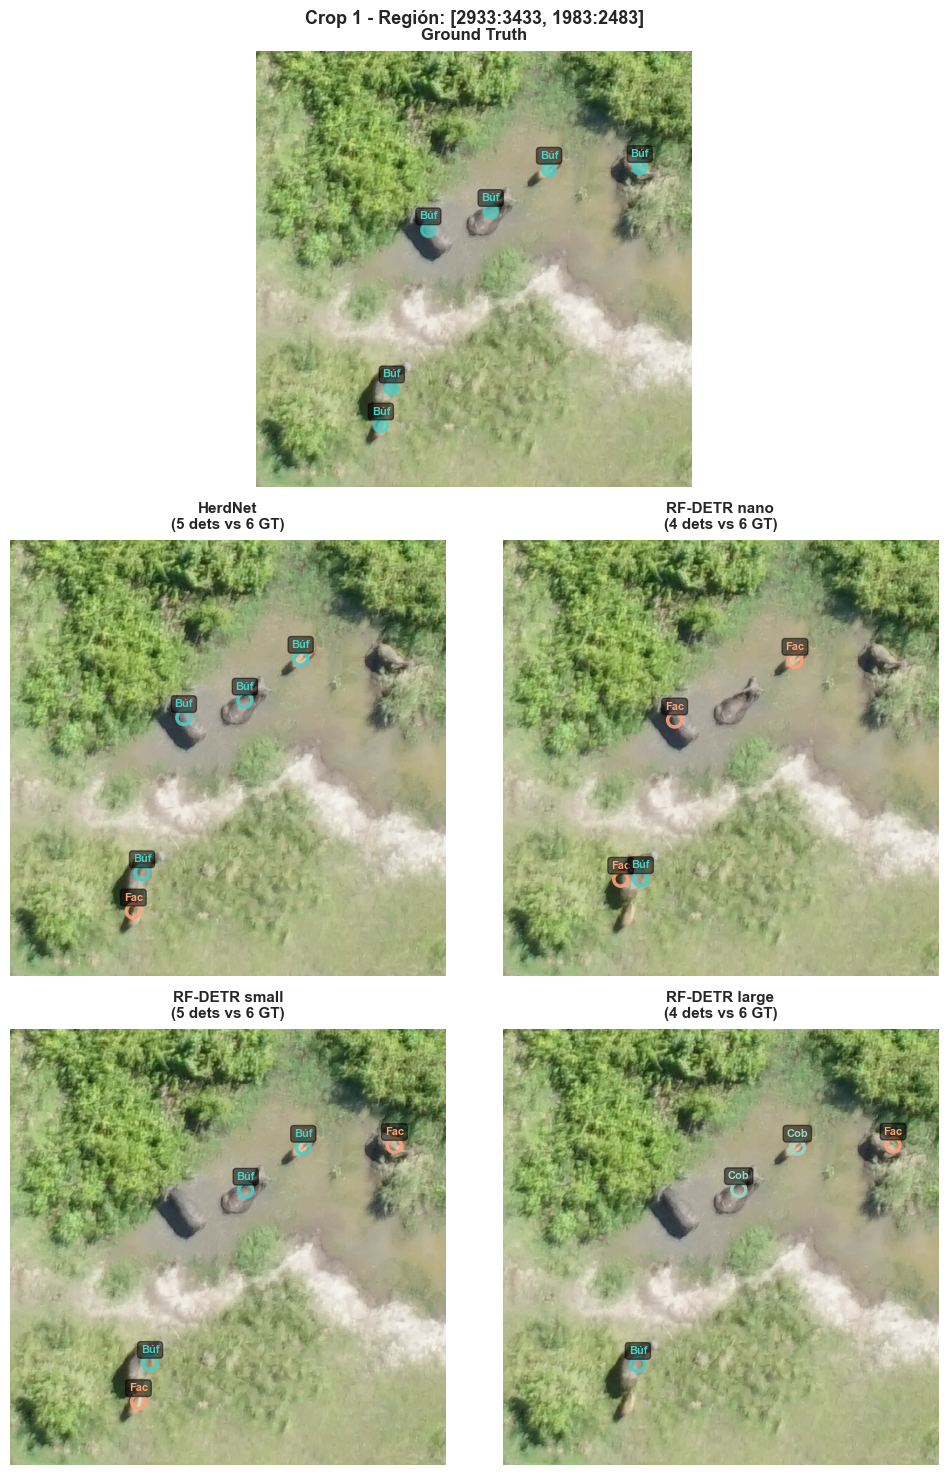
\includegraphics[width=0.9\columnwidth, height=2.25\columnwidth]{static/img/anexo_c_comp_4.png}
%    \caption{Comparación cualitativa del Búfalo. Se observan 6 búfalos.}
    \caption{Qualitative comparison of the Buffalo. 6 buffalos are observed.}
    \label{fig:anexo_c_4}
\end{figure}


\end{document}
